\documentclass[10pt,titlepage,a5paper]{book}
 \usepackage[ngerman]{babel}
 \usepackage[utf8]{inputenc}
 \usepackage{graphicx}
 \usepackage{geometry}
 \usepackage{pstricks}
 
 \pagestyle{plain}
 
%\frenchspacing

\parindent0em 
\parskip1.0ex plus0.5ex minus 0.5ex
%\sloppy

\geometry{left=2.5cm,right=2cm,bottom=3.5cm,top=2.0cm}


 \author{von\\[0.8ex]Johanna Mollydottir}
 \title{\bf\Huge Rinascimento}
 
 \newcommand{\sterne}{\par{\centering ***\par}}

 \newenvironment{tg}{\begin{quote}\em}{\end{quote}}
 
 
 
 \newenvironment{dichter}{\begin{flushright}}{\end{flushright}}


\newcommand{\changefont}[3]{
\fontfamily{#1} \fontseries{#2} \fontshape{#3} \selectfont}


 \begin{document}
 
 
 \changefont{ppl}{m}{n}
 
  %\maketitle
  
 \begin{titlepage}
 

%\includegraphics[width=0.9\textwidth]{/home/felicitas/133_1.JPG}

\begin{pspicture}
(0cm,0cm)(0cm,0cm)
\rput[tl](-2.5cm,2.35cm){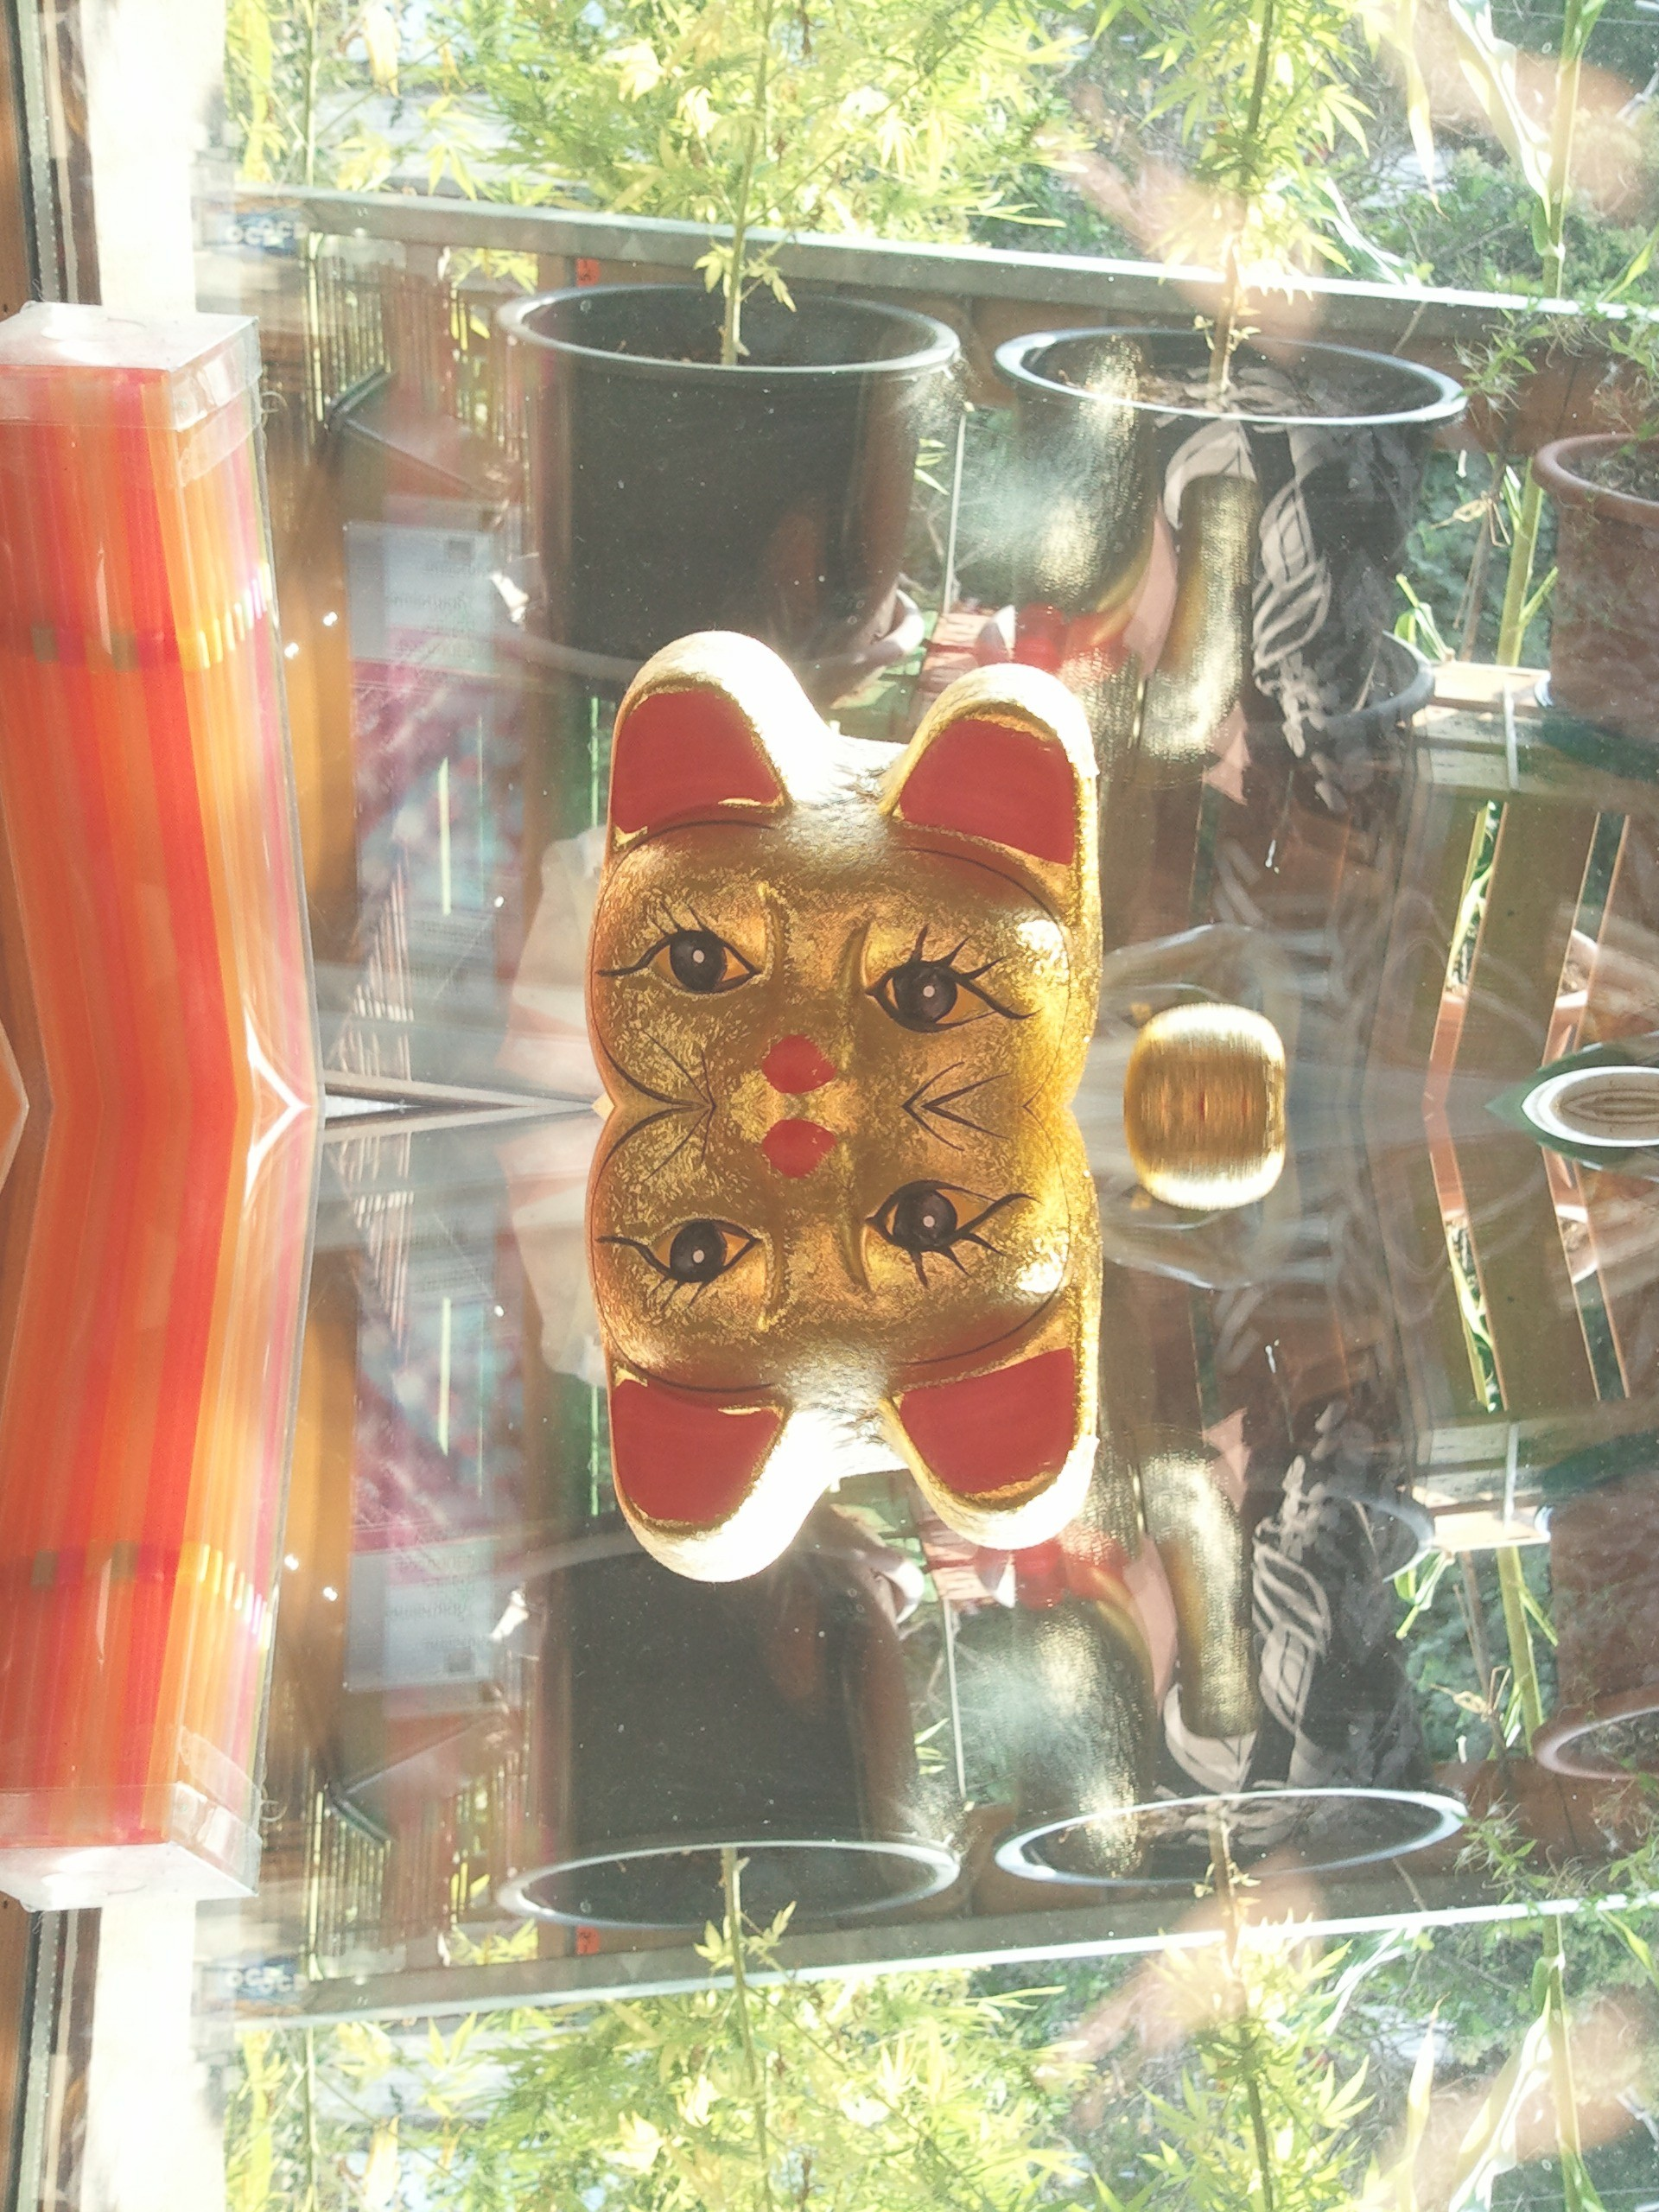
\includegraphics[width=\paperwidth,height=\paperheight]{mitz1}}
\end{pspicture}
 
 
 
   \vspace*{0.25\textheight}
   {\Huge\bf Rinascimento}\\[1.5ex]
   Johanna Mollydottir\\[24.0ex]
   \today
 
 \end{titlepage}


\thispagestyle{empty}


\chapter*{Für}

Meine Mutter

\chapter*{Prolog}
\addcontentsline{toc}{chapter}{Prolog}




„Eine Gabe ist eine Aufgabe.“
\begin{dichter} Käthe Kollwitz\end{dichter}

Sind Sie, verehrter Leser,  auf die Welt gekommen, vergessend, was vorher war?

Sie leben,  atmen, erfahren, begreifen Ihr Dasein als eine Abfolge des sich fortfahrenden „Jetzt“, beginnend mit den ersten Erinnerungen Ihres jetzigen Lebens- einzigartig, neu und einmalig?

Sie leben und erinnern sich nicht? Welche Gnade.

Bei mir ist es anders, dieses  mal.

Denn ich erinnere mich.

Meine Erinnerung ist gross, sie quillt hervor aus allen Ritzen meines Seins.

Glauben Sie an Reinkarnation?

Stellen Sie sich vor, Sie haben das eine oder andere Leben gelebt, \dots und würden sich daran erinnern. Sie erinnern sich ein Feldherr zu sein, \dots Sie riechen den Schweiss und das Blut, \dots spüren den Triumph des Sieges, den Rausch der Macht\dots, denken an die Freuden, die die Weiber bereiten, \dots und finden Sie sich wieder in dem Körper einer Frau, mittleren Alters, verheiratet, zwei Kinder, Auto, Haus und Hund\dots

Wer sind Sie?

Wie viel des einen Lebens gehört zu dem anderen?

Wieso leben Sie dieses?

Ach, seliges Vergessen.

Sie „glauben“ nicht an Reinkarnation?
 
Na, und?

„Glauben“ Sie an den Eiffelturm?

Warum? Haben Sie ihn selbst gesehen? Wenn nicht, woher „wissen“ Sie von seiner Existenz? Von Bildern? Erzählungen anderer?

Dabei ist es nicht schwer sich zu erinnern. Wir erinnern uns ständig, nur, wir wissen nicht, dass wir uns an ein vergangenes Leben erinnern, glauben, es seien Motivationen, Konsequenzen des jetzigen Lebens, aus denen heraus wir handeln.

Was, wären wir ein Puzzle. Ein Puzzle unserer vergangenen Leben, das sich neu fügt, neue Teile einfügt, die das Bild erweitern. Erweitern für das nächste Puzzleteil, bis es vollkommen und harmonisch ist, sich alle Teile zu einer Einheit fügen.

Wo beginnt die Geschichte, die Verschlingungen und Lösungen? Wo beginnt es, wenn die Vergangenheit vorbei ist, sich selbst aber wieder und wieder neu gebärt ins Jetzt. Verändert sich die Vergangenheit nicht mit jedem Gedanken, der sie neu beschwört? Sie verändert mich im gegenwärdtlichen Sein, wann immer ich ihr Raum gebe und sie verändert die Räume in mir, die sie betritt. In diesen Gedanken öffnet und verschliesst sie Türen. Türen, die die eine Zukunft öffnen oder schliessen. Es gibt keine Vergangenheit und die Zukunft entspringt immer neu der Kreation der Gedanken.

Die Flut und Ebbe, der Sturm und die ruhige Regung von Gedanken und Emotionen erschaffen uns sekündlich neu. Es gibt für den Körper Zeit und Raum, den Anker, in der orientierungslosen Flut der Gedanken. 

Alles ist Maya! Maya, die grosse Illusion. Trug- und Wahrbild. Theater, Theater der Seele!

Vorhang auf für Maya.



\part*{Teil I}
\addcontentsline{toc}{part}{Teil I}


\section*{Il paradiso I (Oldendorf 1975-1977)}
\addcontentsline{toc}{section}{Il paradiso I(Oldendorf 1975-1977)}



„Du bist die Frau und ich bin der Mann! Und nun machen wir noch ein Kind.“ „Okay!“ Johanna legt sich auf die Matratze. Sie ist aufgeregt.

Es ist heiss auf dem Dachboden. Die Sonne scheint in das Fenster und taucht den Giebel mit dem dunklen Holz ins Licht. Und die Hitze, die sich dort zur Mittagsruhe gelegt hatte, hüllt die Haut mit zwickenden Fingern ein.

Gleich bekomme ich ein Kind, denkt Johanna und ist besorgt, denn sie weiss nicht, wie das Kind in ihren Bauch passen wird.

Conny legt sich ganz vorsichtig auf sie. Die Bäuche berühren sich und zwischen den Beinen spürt Johanna das weiche Glied des Freundes ihre Vagina berühren. Nein, nein, mit Kindern will Johanna es nicht versuchen.

Beide springen auf, auseinander mit klopfendem Herzen, ist es zu spät? Aber Johannas Bauch ist wie zuvor. Schwitzend sehen sie sich an. Und die Hitze zwickt mit langen Fingern, die nackte Haut und sie spüren sich nackend, sie spüren, der Mann und die Frau, sie warten.

„Aber wir heiraten später, wenn wir gross sind!“ „Ja, und ich werde Müller und habe eine eigene Mühle auf dem Hof und einen Esel!“ „Mit der Mühle ist in Ordnung, aber ich weiss nicht, ob sich meine Kühe mit dem Esel vertragen?“ „Aber Müller brauchen einen Esel!“ „Na, gut.“

Johanna und Conny steigen auf ihre Fahrräder und fahren zu Connys Bauernhof. Der Hof liegt einsam eingebettet in den satt grünen, von Knicks umrandeten Koppeln.

Ein kleiner Hof mit dreissig Kühen, Kälbern und einigen Feldern ringsum. Einer Grossmutter, die kaum ihren Altenteil verlässt und griesgrämig die dünnen Finger aneinander  reibt. Sprechend dicht mit ihrem dünnen, scharfkantigen Gesicht heranrückt und spitze Bemerkungen ausstossend wie ein Huhn zurück ruckt, das Gesicht verzogen.

Die Bäuerin kräftig mit geröteten Wangen, dunklen, kurzen Locken, ist grösser als ihr Mann Klaus. Sie liebt es Schauerliches herauf zu beschwören und dadurch auf Dinge hin zu weisen, die es zu erproben gälte, um für das Leben vorbereitet zu sein.“Aua, aua, mein Zahn, die Kuh hat mich wieder getreten“, jammert sie. Vormelken muss sie, damit die Pfropfen der Melkmaschine die Milch aus den Eutern saugen können.

Bei den gutmütigen Kühen üben sich die Kinder, aber Johanna schafft es nicht, der rosigen, rauen, wackeligen Zitze einen Tropfen Milch zu entlocken. „Drücken und ziehen musst du.“ Conny lacht, während zwischen seinen Fingern die Milch aus dem Euter spritzt. Wie gut, dass ich ja Müller werde, denkt sich Johanna, der Conny muss seine Kühe selbst melken.


\section*{La morte I}
\addcontentsline{toc}{section}{La morte I}


Vor dem Bauern hat Johanna Angst, der spricht selten und poltrig, laut und weiss von Schlimmeren zu berichten als seine Frau. Er verengt seine wässrigen, hellblauen Augen zu Schlitzen und sein Gesicht ist feuerrot, umrahmt von gelben, zerzausten Haaren.

Er lässt die Kinder auf dem Trecker mitfahren. Hinten angehängt eine Maschine um Löcher für neue Zaunpfähle zu bohren. „Wenn du da, an diese Stange mit dem Kopf stösst, gehst du tot.“ Der Bauer schaut Johanna scharf an. Zitternden Leibes sitzt Johanna auf ihrem metallischen, Kissen gepolsterten Sitz, die Finger um die Stange gekrallt, die sie mit dem La morte bedroht.

Der Trecker ruckt und kippt, während er über die Koppel fährt und der Bohrer sich in die Erde dreht.

Da! Der erste Schlag an den Kopf. Johanna blinzelt überrascht, sie ist nicht tot\dots Aber sie ist sicher, sie wird es bald sein. Der Trecker springt und bockt wie ein junges Fohlen, unvorhersehbar und der Kopf springt wieder und wieder gegen die Stange. Wie lange wird es dauern\dots Johanna taucht in sich selbst ein, so weit es geht. Jetzt ist eine Schutzschicht wie dickes, wässriges Glas zwischen ihr und der Welt, sie kann Conny und den Bauern nicht richtig sehen und hören, aber dort ist es sicherer.

Warum lacht Conny? Die Freude kann Johanna nicht verstehen. Der Freund ist ganz unbekümmert und scheint keine Gefahr zu spüren.

Am Ende der Fahrt ist Johanna enttäuscht, sie lebt und fragt sich, ob sie um eine Erfahrung betrogen wurde oder nur um den Glauben in die Worte des Bauern.



\section*{Il paradiso II}
\addcontentsline{toc}{section}{Il paradiso II}



Es ist ein beschauliches Dasein. Der Geruch der Marsch hüllt alles ein. Moorig, wässrig vom warmen Sonnenlicht ausgelöst, verwandelt sich die schwere Erde in kräftigen, säuerlichen-süssen, holzigen Geruch, der ummantelt, nicht durchdringt. Durchbrochen von den zahllosen Knicks, die mit Büschen, losem Strauchwerk und kleinen Bäumen die Wege und verschiedenen Koppeln säumen, gibt das flache Land grosszügig die Himmelskuppel frei. Eine grünes Brett unter einer hellblauen, dunstigen Käseglocke. 

Eine aquarellige Nass-in-Nass Landschaft, dominiert von den Himmelsvariationen und dem, weit in die Ferne in immer hellerem, verwischt Geschichtetem, sich verlierenden Blick. Mal zeigen sich weisslich, milchig, von einer verschleierten Sonne durch lichtete Wolken, der Maler hat das nasse Blau mit einem trockenen Pinsel durchfahren und die beiden unterschiedlichen Flächen machen sich miteinander vertraut. Mal strahlt Blau. Mal ziehen in endloser Formation, auf Schnüren hintereinander aufgeperlt, dicke, flauschige,  von unten platt gedrückt und grau, Cumuluswolken mit dem Wind aus dem Westen.

Die Kinder sind ganz für sich. Es braucht unter der Käseglocke keine Erwachsenen. 

Der kleine Fluss hinter dem Wäldchen bei Johannas Haus ist tabu. Und der Garten der einzigen Nachbarn. Vor dem Haus ist die Landstrasse, die nach Oldendorf führt, dahinter lehmig, gelb die Kiesgrube. Dort sind die Kinder selten. Neben dem Haus ist ein Wäldchen und auf der anderen Seite das gleiche Haus mit den Nachbarn, Auffahrt, Feldweg zu Connys Hof. An der Landstrasse dann ein kleines Stück weiter das Kraftwerk indem der Vater arbeitet.



\section*{Humunculus}
\addcontentsline{toc}{section}{Humunculus}



Gasturbinenkraftwerk. Zwei grosse Klötze nebeneinander mit drei grossen, silbrigmatten Schornsteinen, die weithin sichtbar nach jeder Ausfahrt das Zuhause ankündigen. Zwei Gastanks, rund sind sie und riesig. Es ist eine summende, brummende, vibrierende Welt. Sie riecht nach Öl und Metall, der Geruch beisst in der Nase wie der vom Kuhmist. Aber dieser Geruch fühlt sich an wie kleine, tote Nadeln, und der ranzigen Schwere von Erdöl, dem Leichensaft von Mutter Erde, er hüllt nicht ein wie ein müffelnder, warmer Pelz, sondern tastet vielmehr ab, er durchdringt und sucht,\dots Dann gibt es den Geruch vom Büro, von altem Papier, Arbeitsanzügen, Holzschränke, Kaffee und dem kalten Rauch von Papas Pfeife, der ist wie Heimat.

Wenn Johanna hinter den haushohen Turbinen in die hintersten Winkel der Werkhalle schleicht, es, trotz Beleuchtung, dunkler wird, die Füsse auf dem Laufgitter einen mehrstimmigen, federnden Klang erzeugen, die Rohre, gelb und rot lackiert, die Ventile, Rädchen und Räder zum drehen, aus ihren Winkeln vorrücken, Gesichter bekommen und sie anstarren, dann wird sie vom Grauen ergriffen und rennt zurück zum Eingangstor, das die ganze vordere Seite der Halle ausfüllt und offen und grosszügig Tageslicht herein lässt. Der Vater wäscht seelenruhig das Auto oder bastelt daran, denn Johanna ist nur im Kraftwerk, wenn es Wochenende ist und der Vater sich seinem Auto widmet. Der Vater weiss nichts, von den geheimnisvollen Wesen, die in  der hinteren Ecke der Halle lebendig werden. Und im Tageslicht betrachtet, findet Johanna selbst, dass dort ausser Maschinen und Rohren nichts sein kann,\dots Sie schleicht zurück, um sich zu beweisen, dass alle Dinge Dinge sind, steife, starre Dinge\dots

Fasziniert beobachtet Johanna, während sie sich erneut an schleicht, wie die Angst in ihrem Inneren wächst und wächst, mit den beruhigenden Gedanken und dem Vertrauen ringt und plötzlich vorschiesst und sie mit Entsetzten ausfüllt und dann rennt sie auch schon zurück. Je mehr sie sich zur Vernunft zwingt, je langsamer sie Schritt für Schritt ins Dunkle geht, sich genau umschaut und alles betrachtet, um so heftiger kommt die Angst.
Es ist ein tolles Spiel.



\section*{Credo I}
\addcontentsline{toc}{section}{Credo I}



Abends ist Johannas liebste Zeit auf der Schaukel. Wenn sie auf der Schaukel schwingt und die  Sonne langsam den Weg zum Horizont nimmt, der Himmel heller als am Tag weiss-dunstig sich bereit macht die Farben des Abendrotes auf zu nehmen. Die lang gezogenen Wolkenstreifen zartes Rot und Orange, zu Beginn hellstes Goldgelb, Farbklängen gleich, in die Weite musizieren. Mit dieser Musik vibriert das Herz, immer stärker und tiefer. Die Schaukel schwingt den Bauch, lockert ihn, öffnet jede Zelle, damit das Licht eindringen kann. Heben und senken, der Bauch, der Körper werden schwerer und ruhiger, bis sie selbst aufgelöst mit dem Licht, den Farben klingen. 
Nichts berührt den Kopf, der darf still sein, der Rest ein riesiges Lauschorgan, selbst Wellen der Zufriedenheit verströmend. Im Kern der Engelsmusik, sie spiralt gleichermassen darum, die Leere, all-liebende, alles und nichts seiende Leere.

Ein Auto kommt auf der Landstrasse hinter dem Jägerzaun vorbei gefahren, von der Kupplung gebogenes Motorengeräusch, das schnaufende Auto wird in seiner Fahrt gebremst, Ortseingang. Der höher sich verbreiternde Autoklang vervollkommnend die Musik um Endliches. Das Auto ist Bewegung -bewegen, Weg.
 


\section*{La memoria}
\addcontentsline{toc}{section}{La memoria}



„Mama, Mama, schau mal mein Bild an! Mama wach auf, schau!“ Johanna ist zu den schlafenden Eltern ins Schlafzimmer gestürmt und springt auf das grosse Bett. Die Mutter richtet sich verschlafen auf: „Was?“ „Schau doch, wie ich gemalt habe!“ Der Mutter wird ein Blatt mit kleinen Figuren unter die Augen gehalten. „Mmh? Ja, schön hast du das gemacht.“ „Ich hab die Haare anders gemacht und jetzt sehen sie wie richtige Menschen aus!“ „Prima, komm, geh leise wieder raus, bevor der Papa auch geweckt wird. Ich komm bald und mach Frühstück.“ Johanna geht leise, verzückt aus dem Schlafzimmer und malt gleich ein weiteres Bild auf dem die Menschen viel mehr wie Menschen aussehen als vorher. Johanna hat lange probiert und verschiedenes getestet, sie ist glücklich und stolz, dass sie eine neue Methode gefunden hat, Menschen gut zu zeichnen.

Wenn die Eltern am Wochenende länger schlafen, sitzt sie oft und malt, die Mutter hat ihr dann eine Schüssel mit Kellogs Smacks hingestellt, die knappert sie. Erst jedes einzelne, wie eine Kostbarkeit, dann mehrere, eine Handvoll und zum Schluss hält sie sich die Schüssel an den Mund und mampft die süssen Körner gierig in sich hinein. Sonst weckt sie die Eltern nicht, aber an diesem Tag gelingt ihr zum ersten mal ein kleines Wunder, sie schafft es Dinge zu zeichnen, wie sie sie sich vorstellt und sieht. Bei diesem ersten Mal-Erlebnis ist Johanna vier Jahre alt.



\section*{Il paradiso III}
\addcontentsline{toc}{section}{Il paradiso III}



„Komm, der Mist fährt auf den Misthaufen.“ Johanna und Conny stürmen aus dem Kuhstall. In der Rinne hinter den Kühen fahren die Schieber hin und her, klappen sich ein und aus und schieben die grünen, breiigen Haufen Stück um Stück auf das Förderband zu. Dieses steht hoch aufgerichtet vor dem Misthaufen und vergrössert diesen portionsweise um weiteres Grün.
Erwartungsvolle Spannung, wie gross wird der Haufen, der als nächstes herabstürzt, sein? Wie weit wird er spritzen?

Es ist eine Frage des Könnens, den Haufen, der hochgefahren kommt, einzuschätzen, im richtigen, aber letzten Moment vor den grünen Spritzern zu flüchten.

Im Inneren des Stalls fressen die Kühe gasend ihr Abendheu, während sie gemolken werden. Es muht von den Kühen, es klirrt von ihren Bügeln, durch die sie ihre Köpfe schieben, die sich dann um ihren Hals schliessen. Johanna findet es traurig, dass die Kühe sich, sind die Bügel geschlossen kaum bewegen können. Weiter surrt die Melkmaschinen und gibt gleichzeitig ein klackerndes Geräusch wieder, mit dem die Milch rhythmisch durch die durchsichtige, verstaubte Leitung pulsiert. In der Milchkammer steht eine von Connys Schwestern und giesst von der frischen Milch in Eimer. Die bringen Conny und Johanna den kleinen Kälbern. 

„Schau, meins ist schon ganz zahm!“ “Meins auch!“ Sie müssen die Eimer gut fest halten, denn die hungrigen Kälber stossen kräftig ihre Köpfchen in den Eimer um jeden Tropfen Milch zu schlecken, hinten wackeln und zittern die kleinen Schwänze. Nach der Trinkzeit lassen die Kinder die Kälbern eine Weile an ihren Fingern saugen. Die raue Zunge schmiegt sich an die Finger, die oben von dem zahnlosen Kiefer geknetet werden. Es schmerzt. Johanna freut sich aber, denn sie kann auf  das kleinen Kalb Acht geben. Mit dem Eimer in der Hand laufen die Kinder in die Tenne, jeder macht einen Griff in das Schrot und ab in den Mund damit. Im Winter läuft die Häckselmaschine, die aus den Futterrüben kuh- und kindgerechte Schnitze macht, die bei laufender Fahrt aus der Maschine geklaubt werden.



\section*{La morte II}
\addcontentsline{toc}{section}{La morte II}



Im Winter spielen Johanna und Conny in der Scheune verstecken. Sie ist bis unter das Dach mit Heu und Strohballen gefüllt. Die Kinder sollen das Stroh nicht durcheinander bringen und damit spielen- unmöglich. Für kleine Höhlen reicht das lose Stroh.

„Komm, wir springen von den Ballen dort oben!“ „ Ich traue mich von dem dort, der ist höher!“ Conny steigt höher und Johann will nicht nachstehen. Ein Moment hebt sich der Körper empor, schwingt mit der Luft und kehrt zurück auf die feste Erde. Sie können nicht genug bekommen und höher, höher\dots Der Aufprall staucht die Beine, der Schmerz wird grösser, die Luft wird aus den Lungen geschleudert, wenn sich der Leib fester und fester nach dem Höhenflug an den Boden presst. Es geht um die Ehre.

Conny springt. Bleibt liegen. Johanna klettert schnell herunter. Conny liegt da und rührt sich nicht mehr, die Augen sind geschlossen.

Johanna stürmt ins Haus und holt den Bauern und Bäuerin. Die Angst kommt mit, die Angst , die kribbelige, die erregende Angst vor dem Tod.

Conny ist wieder da. Die Eltern erleichtert, stürmen auf Johanna ein: „Conny hätte sterben können, du weisst, dass das Verboten ist! Das dürft ihr nicht\dots“ Johanna ist getroffen und verletzt, warum schreien der Bauer und die Bäuerin mit ihr herum, schliesslich war es Conny, der sich gestossen hat. Es ist nicht recht. Johanna kneift fest die Lippen zusammen und sagt nichts. Aber das Gewissen nimmt ein Stück Schuld zur Untermiete ins Herz.



\section*{Gnomus}
\addcontentsline{toc}{section}{Gnomus}



Am Abend fährt Johanna heim. Allein. Vorn, am Fahrradlenker, baumelt eine Tupperkanne mit frischer Milch. Der Weg besteht aus zwei Betonplattenspuren, getrennt von Gras. An den Seiten hat es Gras und an beiden Seiten Knicks mit Büschen und Sträuchern, kleinen Bäumen. Ein einfacher Weg, ein klarer Weg. Hinter der Kreuzung kommt das kurvige Stück. Johanna fürchtet sich vor dem kurvigen Stück, ihr ist jedes mal, als werde sie beobachtet, als wollte etwas hinter dem Erdwall hervorspringen und ihr den Weg versperren. Es ist keine besondere Ecke, die dunkler wäre oder enger, es ist nichts zu sehen und doch müssen unsichtbare, wütende und raubende Wesen hinter dem Wall sitzen, auf Beute lauernd. Dort fährt sie, so schnell sie kann. Einmal, als sie es besonders eilig hat, rutscht der Reifen über die Betonplattenkante auf die ausgewaschene Grasspur, bleibt widerspenstig, schliesslich bockt das Fahrrad und Johanna fällt.

Sofort taucht Johanna unter, nichts hat mehr Platz unter ihrer Seelenwasserkuppel ausser namenloser Schrecken\dots Nicht den kleinsten Schmerz spürt sie, während sie mit fliegenden Händen den Lenker greift und im Laufen auf das Fahrrad springt und wild bis zur letzten Kurve strampelt. Auf dem letzten, geraden Wegstück spürt sie ihr Herz im Mund klopfen und bemüht sich es wieder runter zu schlucken. Es dröhnt in den Ohren. Die Knie melden sich mit dem Schmerz vom Aufprall,  langsam geht die Fahrt nach Hause. Links der hohe, dicht bewachsene Knick und rechts eine Koppel, die die Blick auf den Abendhimmel öffnet. Über dem Kopf, hoch oben, die Strommasten und Leitungen, die den Strom fort bringen, den der Vater im nahen Kraftwerk gemacht hat. Es summt in der Luft.



\section*{Il uomo nero}
\addcontentsline{toc}{section}{Il uomo nero}



Conny und Johanna steigen auf die Fahrräder, sie wollen zu Johanna fahren. Jeder auf einer der von Gras getrennten Betonplattenspuren. Der klare Weg, ihr Weg, den kaum mal ein Spaziergänger betritt ist heute anders, still, kein Vogel ist zu hören, die Bäume auf den Knicks zu beiden Seiten wirken vor dem nebelig-trüben Himmel dunkel, die Luft legt sich dick, schwül auf die Augenlider.
 Ihnen entgegen kommt eine schwarze, in eine lange Kutte gehüllte Gestalt. Es ist ein Mann mit schwarzem, zerzaustem  Haar, einem langen Bart und bleichem, blassen Gesicht. Als er die Kinder sieht, bleibt er stehen, breitet er die Arme über den Kopf und beginnt mit lauter Stimme in einer fremden Sprache zu sprechen.
 
Sie bleiben stehen. Die Stimme saugt an den Ohren, sie will die beiden Kinder einfangen. Nach dem ersten lähmenden Schrecken, drehen Johanna und Conny um und fahren mit fliegenden Beinen zurück zum Hof.

„Da, da kommt ein schwarzer Mann. Er kommt, er kommt!“ „Ein ganz schwarzer Mann, der ruft.“ Schreiend und keuchend kommen die Kinder in die Küche gestürzt. Das rote Tier Angst löst sich von ihnen und springt\dots Die Erwachsenen springen auf. „Du bleibst drinne!“, der Bauer schaut Johanna streng und besorgt an, die anderen stürmen aus dem Haus. Conny darf mit raus. Der einsam gelegene Hof hat zwei Einfahrten und Johanna sieht den Bauern zu der einen Einfahrt gehen, zu der, die dem Wanderer am nächsten liegt, einen Besen mit kräftigen Stil in der Hand. Die Bäuerin nimmt eine Mistgabel. Connys grosse Schwestern gehen zu der anderen Einfahrt. Es kribbelt in Johannas Bauch. Wer ist der Mann? Was wird der Bauer mit ihm machen? Kann er ihn besiegen?

Wut und Angst wandern mit den Erwachsenen in den Toreinfahrten mit. Das rote Tier, das von einem zum anderen hetzt und sich die Leftzen leckt, auf Futter wartete. Es möchte toben und Blut, es drängt sich zu den Menschen, umspringt sie. Ganz plötzlich sieht Johanna es und es ist gruseliger als der schwarze Mann, der allein den Weg herauf kommt. Johannas Herz klopft heftig, wenn der Bauer den Mann schlägt? Mit dem Besenstiel. Sie kann die Einfahrt nicht sehen. 

Johanna kommt es vor wie eine Ewigkeit, die sie alleine am Küchenfenster verbringt. Conny läuft auf dem Hof hin und her. Die Erwachsenen reden aufgeregt miteinander und schauen immer wieder den Weg hinunter. Dann wird das  Tier kleiner, unruhig dreht es sich im Kreis, entfernt sich langsam, von den Menschen, wird von einer unsichtbaren Wand von ihnen weg geschoben.
Schliesslich sammeln sich alle in der Einfahrt, die dem Wanderer am nächsten liegt.  

Von den Mann ist keine Spur zu sehen! Er kommt nie an der Einfahrt an!
Wohin ist er auf dem schmalen, von Knicks und Feldern umgebenen Weg verschwunden\dots

Die Erwachsenen verstauen Besen und Mistgabel und lachen befreit, vorwurfsvoll, was Kinder für eine blühende Phantasie haben\dots Widerwillig verschwindet das rote Tier einen Rest Wut zurücklassend und Scham, die Erwachsenen können sich nicht in die Augen sehen.



\section*{Credo II}
\addcontentsline{toc}{section}{Credo II}



„Natürlich gibt es den lieben Gott!“ sagt Conny. 

„Bist du sicher?“

„Ja, der wohnt im Himmel und hat einen langen Bart. Der sitzt dort auf einer Wolke und wenn man betet, dann hört er das. Und er sieht alles, was du machst.“

„Und das Paradies?“  

„Das ist im Himmel, dort kommt man hin, wenn man stirbt. Oder in die Hölle, dort brennt es. Da kommen die Bösen hin.“ 
„Kann jeder mit dem lieben Gott reden?“ „Ja, man sagt, lieber Gott im Himmel und dann was man möchte\dots“


„Wenn ich Tod bin, bleibe ich nicht im Sarg liegen?“


„Nöh, dann kommst du zum lieben Gott\dots“

Ich liege nicht im Sarg als würde ich tief schlafen, denkt Johanna. Ich muss nicht im Sarg liegen und die Würmer kommen und fressen mich, während ich schlafe. Ich muss nicht im Sarg liegen, während die Würmer meinen Körper fressen und ich nicht träumen und nicht aufwachen kann\dots Ich kann nicht aus versehen aufwachen, wenn die Würmer meinen Körper zerfressen\dots

Wenn ich sterbe, darf ich weiterleben\dots bei dem lieben Gott im Himmel.

So glaubt Johanna still und heimlich, während ihr Kopf verzweifelt versucht den mütterlichen, kommunistisch-atheistischen Vorstellungen des Todseins zu folgen.


\section*{La principessa I}
\addcontentsline{toc}{section}{La principessa I}



Johanna greift in die Verkleidungskiste und holt ein glänzendes Kleid hervor und die schicken Sandalen mit Riemchen und kleinen Absätzen, solche, wie sie grosse Frauen tragen. Damit stolziert sie im Garten auf und ab.
 Wunderbar. 
 
 „Mama, darf  ich die Sandalen zum Einkaufen anziehen?“ „Nein, Johanna, das weisst du doch! Die Schuhe sind nicht gut für deine Füsse, weil die Einlagen nicht hineinpassen.“ “Aber Oma Frankfurt hat sie mir geschenkt.“ „ Johannaaa, nein!“ Johanna findet das ungerecht, warum darf sie keine richtigen Mädchenschuhe anziehen, nur diese hässlichen Sandalen, die hinten geschlossen sind, Babyschuhe.
 
Faschingszeit im Kindergarten. Plötzlich heisst es sich verkleiden. Johannas Mutter hat ihr ein Funkenmariechen Kostüm gekauft. Aber Johanna weiss nicht, was ein Funkenmariechen ist. Die rote Jacke mit den goldenen Knöpfen, sieht aus wie die eines Soldaten und das weisse Faltenröckchen sieht wie ein normaler Rock aus. Der roten Hut, ein Dreispitz, sieht auch aus wie für Soldaten. 

Aber Johanna darf die Sandalen mit Riemchen anziehen. 

Johanna bekommt einen Beutel mit Bonbons. Sie darf sie aber nicht essen. Ein Funkenmariechen wirft die Bonbons in die Luft, damit die anderen sie fangen und essen können. Das widerstrebt Johanna, warum soll sie all die Bonbons weggeben. Johanna versteht nichts, nicht, als was sie verkleidet ist und nicht, warum sie Bonbon zum Wegwerfen bekommt.

Aber, dass ihre Freundin Britta als Prinzessin zum Fasching darf, das versteht Johanna. Wie hat Britta das gemacht? Sie hat  nicht nur ein langen, goldgelben, glitzernden Rock und ein goldiges Oberkleid, nein, sie hat sogar ein kleines, glänzendes Krönchen mit einem Schleier auf dem Kopf. Und Britta schreitet umher und vergisst nicht, den Schleier, als ob er ihr langes Prinzessinenhaar wäre von der einen Schulter zu streichen und dann von der anderen zu streichen und den Kopf nach hinten zu werfen. Wie gern wäre Johanna eine Prinzessin\dots

Die Kinder tanzen und springen. „Johanna, du musst noch die Bonbons werfen und verteilen“, die Mutter hat den Beutel mit den Bonbons in der Hand. Johanna wird es heiss und dann läuft ein kalter Schauer den Rücken runter. Sie schämt sich und sie hat Angst. Wie soll sie das machen? Alle Kinder werden sie bedrängen, schreien und nach den Bonbons grabschen. Johanna möchte am liebsten den Sack, gefüllt wie er ist, mit nach Hause nehmen und das nicht, weil sie die Bonbons essen will. 

Die Mutter macht ihr Mut: “Los, Johanna, wirf` die Bonbons einfach zu den Kindern“. “Wie soll ich das den machen?“ Johanna ist verzweifelt.  „Du musst doch nur werfen!“, sagt die Mutter fassungslos, sie versteht nicht, warum Johanna es nicht macht. 

Die Bonbons fliegen, an die Wand und unter die Turnbänke, die rundherum aufgestellt sind. „Johanna, du sollst die Bonbons zu den Kindern werfen. Am Rand und unter den Bänken findet sie keiner“. Es dauert eine Zeit bis die anderen merken, dass Johanna mit Bonbons wirft. 

Dann kommt Silvia, die Tochter von der strengen Aushilfskindergärtnerin, die nur zu ihrer Tochter nett ist und alle anderen Kinder ausschimpft. „Darf ich auch Bonbons verteilen?“ Johanna kennt Silvia nicht gut, sie spielen an den zwei Tagen, an denen Johanna im Kindergarten ist, nie miteinander. Aber Silvia ist die Tochter von Frau Potthof und deshalb hat sie das Sagen bei den Kindern.  Silvia lächelt und wirft elegant die Bonbons. Die anderen Kinder drängen sich um sie und sie verteilt die Bonbons mit vollen Händen, als wäre sie das Funkenmariechen. Der Sack ist schnell leer, dass für Johanna kaum welche übrig bleiben. Silvia lacht und geht wieder Hüpfen und Tanzen, wie die übrigen Kinder. 

Und Johanna? Sie taucht in sich unter, ist froh, dass sie der Aufmerksamkeit entgangen ist und traurig, denn, die Mutter ist unzufrieden. Johannas Gewissen meldet sich, du hat es falsch gemacht und die Gier meldet sich, du hast nicht einen Bonbon abbekommen. 


\sterne


Es bietet sich eine neue Gelegenheit eine richtige Prinzessin zu werden. Eine Märchenprinzessin. Im Kindergarten werden beim Sommerfest Märchen aufgeführt. Johanna darf die Prinzessin im Froschkönig sein. Die Kindergärtnerin sitzt mit Johanna an dem Brunnen aus Pappe. „So, Johanna, jetzt stell dir vor, du bist die Prinzessin und dir ist deine liebstes Spielzeug in den Brunnen gefallen. Und nun weinst du!“ Die Kindergärtnerin sieht Johanna erwartungsvoll an. Johanna steht an dem Pappebrunnen, die anderen Kinder sehen zu. Johanna muss lachen und schaut die Kindergärtnerin hilflos an. „Ich zeig`dir wie es geht.“ Die Kindergärtnerin schlägt die Hände vor ihr Gesicht und gibt schluchzende Geräusche von sich:“Huuuuhuhuhuuuh!“ Am liebsten möchte Johanna wieder lachen, aber sie will sich Mühe geben, damit sie die Prinzessin vom Froschkönig sein kann. Johanna spürt wie sich ihr Körper verändert. Sie fühlt ihn stärker und stärker, gleichzeitig verschwimmt ihr die Kindergärtnerin. Sie versucht es:“Huhu, \dots“ Das Gesicht verrutscht und im Bauch ballt sich ein Glucksen zusammen. Johanna lacht, sie will nicht, aber sie muss lachen.
Nein, nein. Die Kindergärtnerin erklärt geduldig, Johanna wäre traurig, genau wie die Prinzessin und sie sollte es noch einmal versuchen.

Johanna wird es ungemütlich, sie möchte Prinzessin bleiben, aber tun, als ob sie weint, wenn sie nicht weinen muss, kann sie nicht. Warum, warum nur, kommt stattdessen ein Lachen aus ihr raus? Die Enttäuschung der Kindergärtnerin kribbeln in Johannas Bauch. Sie fühlt wie ein Stück von ihr tiefer  in sie hinein gesogen wird und sich in einen dunklen Winkel verkriecht. Johanna sitzt in der Taucherglocke. Johanna lacht mehr und mehr, sie kann nicht aufhören, als würde sie weinen. Dann ist Schluss mit dem Froschkönig. 

Johanna bekommt, als einzige, eine neue Rolle. Jetzt ist sie das Dornröschen. Sie weiss, dass die Kindergärtnerin sie zum Dornröschen bestimmt hat, weil sie dabei still mit geschlossenen Augen da liegen muss, das Einfachste auf der Welt\dots Aber, Johanna ist Prinzessin geblieben, eine mit einem unruhigen Gewissen, aber Prinzessin\dots

Zur Aufführung bekommt sie ein schönes Kleid und eine Krone. Die anderen Kinder singen das Dornröschenlied und tanzen um Johanna und ihre Kinderdornenhecke herum. Sie muss lachen, es kitzelt wieder im Bauch, diesmal, weil sie sich freut und dann weil es laut und lärmig ist und Johanna aufgeregt ist und sich wieder untergetaucht anfühlt. Sie kann nur noch ein Drehen im Bauch spüren, die anderen um sie herum, sieht und hört sie wie durch Wasser, weit weg und sie ist plötzlich ganz allein\dots Und deshalb lacht das Dornröschen statt zu schlafen und als der Prinz kommt, da springt es auf und hopst und springt wild mit ihm herum, dass ihm hören und sehen vergeht. 

Einige Wochen später merkt Johanna wieder wie schwer es ist, Prinzessin zu sein und: Johanna ist keine Prinzessin, nicht mal eine schlafende. Die Mutter hat die Fotos von der Aufführung abgeholt und lacht. Denn das Johannadornröschen liegt kichernd und mit aufgestellten Knien auf ihrem Prinzessinenbett, so dass jeder ihre Unterhose unter dem Kleid sehen kann\dots


\sterne


Jedenfalls will Johanna Klonschen haben. Die schicken Schuhe mit der Holzsohle, die alle tragen. Sie bittelt und bettelt und tatsächlich. Es sind nicht die, die sie sich gewünscht hat, sie darf die mit dem Riemen haben. Mit den neuen Schuhen geht sie hin und her, schaut auf ihre Füsse und spürt die harte Sohle am Fuss. Es fühlt sich grossartig, ungewohnt und ungemütlich an. Die Riemchen schiebt sie oben auf den Schuh und dann wieder hinter die Ferse, wieder auf den Spann, wieder an die Ferse, sie kann sich kaum satt sehen. Mit solchen schönen Schuhen muss sie in die Welt, Conny besuchen.

 „Aber nicht mit den Klonschen“, sagt die Mutter. „Bei Conny musst du andere Schuhe anziehen.“ Johanna kann es nicht fassen, sie hat endlich richtige Schuhe und darf damit nicht zu Conny gehen. „Ich pass` doch ganz doll auf.“ verspricht sie. „Aber dann musst du das Riemchen hinten tragen“. Johanna steigt auf das Fahrrad. Ein bisschen böse ist sie schon, wegen den Riemchen, die sind für Babys.  Dennoch,  sie kommt sich wie ein echtes Mädchen vor, eine echte Frau. 
 
Conny zeigt sich wenig beeindruckt über Johannas Schuhe, er hat andere Pläne und es geht über die Koppel im Galopp. „Warte“ schreit Johanna Conny nach, denn sie lernt, dass  Mädchenschuhe den Füssen einige Schwierigkeiten bereiten können, wenn es um Schnelligkeit geht. Conny ist beim Stall angelangt, Johanna hetzt hinter drein. Ein stechender Schmerz fährt ihr in Knöchel, der über einer alten Flasche, die gut versteckt im Gras die Sonne geniest, davon, zur Seite rollt und sie dabei zu Boden wirft. Johanna springt wieder auf, aber sie kann nur humpeln, der Knöchel ist dick geschwollen als sie heim kommt. „Siehst du, ich habe es dir ja gesagt!“ Ja, das hat die Mutter getan und Johanna hat bei der Strommassage, die der Knöchel über Wochen bekommt, Gelegenheit darüber nachzudenken, wie sinnvoll es ist auf die Erwachsenen zu hören. Schuldig, sagt das Gewissen. Warum kann Johanna kein richtiges Mädchen sein?


\sterne



Wenn Johanna mit den Freunden, den Jungen, unterwegs ist, dann fühlt sie sich wirklich als Prinzessin, oder als Mädchen. Und das ist gut. Denn Johanna ist ein starkes Mädchen, eines, das mit den Jungen mithält, keine Heulsuse. Die Jungen, das sind Sönke, Holger, Kai, Heiko und Conny.
Die Jungen sind alle miteinander verwandt und Johanna ist die „Henne“ im Korb. 

Der Sönke, der ist das Mädchen bei ihnen, denn er heult schnell und kann nicht schnell rennen. Und auch beim Weitpinkeln ist er der letzte.- Da kann Johanna nicht mitmachen, aber das macht nichts. Schliesslich braucht es einen verlässlichen Schiedsrichter, der schaut, wer es am weitesten geschafft hat.- Und weil Johanna genauso gut ist wie die Jungen und der Sönke das Mädchen ist, deshalb können auch Kai, der kleine Bruder vom Heiko und Holger, der kleine Bruder vom Sönke und vom Helge, der aber nicht mehr mit ihnen spielt und viel älter ist, nichts sagen. Denn den beiden ist es nicht immer recht ein Mädchen dabei zu haben.

Johanna ist gerne ein starkes Mädchen, sie misst sich mit den Jungen, will die kleinen Wettkämpfe gewinnen. Sie will den Mut und ihre Kraft trainieren. Ein kleines Stück über sich hinaus wagen, und schaffen! Instinktiv spürt sie dabei ihre unbeugsame Stärke, die eigene Verlässlichkeit und, dass beides lebenswichtig ist.

Es gibt viel zu erleben. Bei Conny auf dem Hof und auf den Koppeln, bei Johanna im Garten. Manchmal machen sie Fahrradtouren. Zu dem kleinen, viereckigen Tannenwald, in den sich aber nur die Mutigsten wagen, weil der Bauer, dem es gehört, dort mal ein totes Kalb mit einem Strick um den Hals liegen gelassen haben soll. Es heisst, der Bauer lauere mit der Schrottflinte und würde auf jeden schiessen, der seinen Wald betritt.

Einmal sind sie bei Kai und Heiko zu Hause. Dort sitzen sie ganz artig in der guten Stube und spielen Mensch-ärgere-dich-nicht. Es ist allen ungemütlich. Und sie wissen nicht richtig, wie sie sich benehmen sollen. Im Haus, am feinen Stubentisch fühlen sie sich erwachsen und versuchen sich zu benehmen, das ist langweilig. Aber keiner sagt es. 

Johanna lernt Neues kennen. Sie, die mit dem Conny verlobt ist, bekommt einen Verehrer. Heiko, der älteste von allen, er ist schon 7 Jahre alt, merkt, er ist in Johanna verliebt. Johanna findet das mal gut, nämlich dann, wenn einer von den kleinen Jungen über Mädchen schimpft und dann vom Heiko einen Rüffel kriegt manchmal ist es aber blöd, nämlich, wenn Heiko den Beschützer spielt und nicht will, das Johanna all die „gefährlichen“ Abenteuer mit macht.

Einmal, alle fahren rasend schnell mit ihren Fahrrädern auf dem Feldweg zu Johannas Haus, da fällt Johanna hin. Sie hat von allen das kleinste Fahrrad, die anderen sind weit vor raus, sie rutsch mit dem Vorderrad über die Kannte des Plattenweges, der Lenker fliegt herum, das Fahrrad springt, padauz. Johanna kriecht unter dem Fahrrad vor, sieht die anderen um die Ecke zu ihrem Haus abbiegen und ärgert sich. Oh, wie sie sich ärgert. Wütend steigt sie mit schmerzendem Knie auf ihr dummes, kleines Fahrrad und strampelt hinterher.

Als sie endlich zu hause ankommt, steht die Mutter in der offenen Tür, Heiko liegt vor ihr auf der Auffahrt am Boden: “So ist sie hin geflogen. So, so auf der Seite. Und das Bein war da unter dem Fahrrad.“ „Johanna, da bist du ja, du Arme, ist alles in Ordnung?“ fragt die Mutter besorgt.
 Johanna kocht, warum muss Heiko diesen peinlichen Sturz vor allen Jungen und der Mutter breit treten? Was geht ihn das an? Wieso nimmt er ihren Sturz um sich vor den anderen wichtig zu machen? Sie wollte die Sache lieber für sich behalten, sich wie ein Junge benehmen und tun als sei nichts passiert. Warum will Heiko Johanna wie ein Mädchen behandeln? Er schenkt der Prinzessinnenseite eine ungewohnte und unangenehme Aufmerksamkeit.
 
Als Heiko dann aber mit seinem kleinen Bruder an Johannas Geburtstag morgens früh vor der Tür steht, um ihr sein Geschenk zu bringen, in feinem Hemd und sauberer Hose, fein auf die Seite gekämmtem Haar, wie ein kleiner Herr, ist sie geschmeichelt. Sie will prinzessinengleich nach dem Päckchen greifen.  Aber die Mutter schickt die Jungen wieder nach Hause, sie sollen am Nachmittag kommen, wie alle Geburtstagsgäste.



\section*{Il fico I 
(Landesmuseum Schleswig-Holstein, Schloss Gottorf, Raum der Moorleichen, 1977)}
\addcontentsline{toc}{section}{Il fico I (Landesmuseum Schleswig-Holstein, Schloss Gottorf, Raum der Moorleichen, 1977)}



{\em Ich liege still, begafft  mit angeekelten Blicken bemitleidet. Meine Haare haben sie genommen, damals, das Moor färbt Haare rot.
Mein Kopf ist schwarz und ich liege, schwarz an Leib und schwarz an Erinnerungen, schwarz in der Stille. Begierig kriechen ihre Blicke über mich, meinen Tod, meine Wiedergänger tanzen um sie.

Die bösen Geister trinken aus ihrem Mitleid und sie starren durch die Scheibe.

Ich springe sie an, das kleine Mädchen hinter der Scheibe, sieh her, was sie mit mir, mit uns getan haben. Ich kralle mich in ihre erstarrten Augen, die wiedererkennen, aber nicht begreifen, im Schock geweitet, mich verschlingen. Sieh mich an, meine vertrockneten, vom Strick zerstörten Stimmbänder knistern ihr ins Ohr:

"Ich war du und die, die du werden wolltest, wird ich werden, bis du mich in dir erlöst hast."

Sie trägt mich mit sich nach Hause und ich nehme sie mit jede Nacht\dots
Jede Nacht ertrinken wir im Moor und im Laufe der Jahre zieht sich der Strick, der meine Stimmbänder und meine Luftröhre zerbrach von Innen um ihren Hals.

Sie wird stumm, erstickt an der Stille, in der ich in ihr ertrinke im Moor, jede Nacht\dots

Nacht, um Nacht, um Nacht\dots

Ich liege, sie liegt und die Äste prasseln auf uns, verkrampft im Tod, in der Schande, verewigt am Pranger der Geschlechtlichkeit, ins Moor gegossen, im Schaukasten ausgestellt.

Ich liege in ihr, ich flüstere, ich knistere ihr den Strick um den Hals:
"Es ist das Herz! Törichtes Ding. Es muss schweigen, damit du leben kannst, dass es zwischen deinen Beinen still bleibt. Es ist das Herz."

Sieh mich, ich bin schwarz, schwarz wie die Nacht, wie die Sünde, wie die Offenbarung und die Verheissung. Schwarz und zerspielt\dots

Ich bin Hülle. Ich war Hülle. Aber das Moor, die schlüpfrige, alte Erdenmutter, sie hat mich zur Figur gemacht. Das Moor machte aus mir das Bild deines Schattens.

Ich bin schwarz. Ich bin tot und durchdrungen von der Erde zurückgekehrt, damit sie, die ihr Herz sucht, sich spiegelnd ins Licht wenden kann.}


\section*{Il mondo delli altri (1977)}
\addcontentsline{toc}{section}{Il mondo delli altri I (Dorf, 1977)}



Johanna steigt mit der Mutter aus dem Auto. Heute ist ihr erster Schultag und sie ist aufgeregt. Die Mutter gibt ihr eine grosse Schultüte aus der oben der Kopf eines Barbiepferdes herausragt. Das hat sich Johanna lange gewünscht. Die Schule ist nicht die, an der sie früher immer vorbeigefahren sind, wenn sie in Itzehoe einkaufen gingen und wo Conny und Britta zur Schule gehen. Sie sind lange mit dem Auto gefahren bis zu der Stadt, wo Oma Dorf, Mamas Mama im Nachbardorf wohnt.

Conny ist ein Jahr vor Johanna in die Schule gekommen und brachte von dort einen „Fu“ mit. Einen, aus einer alten Socke genähten, Fingerpuppenhund, der den Kindern im ersten Schulbuch erklärt, wie Lesen und Schreiben geht. Johannas Mutter hat ihr auch einen Fu genäht und die Kinder sitzen mit ihren Fus auf der Hand über das Schulbuch gebeugt und üben Buchstaben schreiben auf Blättern mit Linien.

Und heute darf Johanna selbst in die Schule\dots

Sie ist mit der Mutter in dieser Schule gewesen um ihren Lehrer kennen zu lernen, wie die Mutter sagt. Johanna findet alles merkwürdig. Den muffigen Geruch des Büros, indem sie und die Mutter von zwei Lehrern erwartet werden und deren prüfenden Blicke sind unangenehm. Der junge Lehrer will Johanna einen Ball zu werfen, den sie auffangen soll und Johanna bekommt Angst, denn fangen kann sie nicht gut, aber es geht. Und Rückwärtslaufen soll sie auf einem Strich, der auf den Boden gemalt ist. Johanna scheinen alle die Aufgaben, die ihr der Lehrer gibt, schwierig, dabei ist sie hundertmal rückwärts gelaufen und hat Dinge gefangen, aber, wenn der Lehrer es sagt und sie dabei streng beobachtet, dann fühlen sich ihre Arme und Beine anders an, als gehörten sie ihr nicht.

Zum Schluss darf Johanna ein Bild malen und sie entspannt sich. Wenn sie eine Sache kann und gern hat, dann ist es Malen. Sie malt ein Haus mit Garten und Himmel und Wolken und ist zufrieden. 

Aber der Lehrer ist es nicht. „Das Bild ist doch noch nicht fertig. Was fehlt noch, Johanna?“  Johanna sieht sich ihr Bild an und kann nichts Fehlendes entdecken. „Doch, das Bild ist fertig.“ „Nein, das Haus ist kein richtiges Haus, es hat nur einen Strich rundherum. So sieht kein Haus aus. Du musst es ausmalen.“ Johanna presst die Lippen zusammen. Sie malt nie ihre Häuser aus. Aber, wenn der Lehrer es will\dots Johanna nimmt den Buntstift und beginnt zu malen. Es ist mühsam und Johanna findet ihr Haus wird durch die vielen wirren Striche immer hässlicher. Sie legt den Stift weg. „Johanna, schau, das Dach braucht noch Dachziegel.“ Der Lehrer lässt nicht locker. Also malt Johanna das Dach an. Als sie fertig ist, sieht sie ein Bild, wie sie es noch nie von sich gesehen hat und sie mag es nicht leiden. Und das Gewissen sagt: „Der Lehrer sagt, du kannst nicht richtig malen.“


\sterne

Aber all das ist am ersten Schultag vergessen. Johanna wird heute Lesen, Schreiben und Rechnen lernen und sie geht selbst zur Schule.
Zuerst sammeln sich alle Kinder, die in  die Schule kommen in einem kleinen Haus, das sechs Ecken hat, der Eurythmiepavilion, aber das weiss Johanna ja nicht. Die anderen tragen auch Schultüten. Sie setzten sich vor eine kleine Bühne und die zweite Klasse führt ihnen ein Theaterstück vor, indem es um die Wochentage geht. Während der Aufführung lässt ein Junge seine Schultüte fallen und einige Sachen fallen heraus. Weintrauben hat er in seiner Schultüte. Der Junge tut Johanna Leid, denn sie wollte keine Früchte in ihrer Schultüte und sie freut sich auf ihr Barbiepferd.

Endlich ist die Aufführung vorbei und der Lehrer verspricht, dass sie in die Klasse gehen und ihre erste Unterrichtsstunde haben werden! Für jedes Kind liegt auf jedem Schulplatz ein Heft mit leeren, weissen Seiten und ein Kästchen mit Wachsmalkreide. Johanna wundert sich, sie findet Wachsmaler doof, zu hause malt sie lieber mit Filzstiften. 

Die Kinder dürfen nicht in ihr Schulheft malen, sondern sie bekommen ein Blatt. Der Lehrer, Herr Boss, erzählt den Kindern eine Geschichte. Dann zeigt er auf die Tafel. Auf der einen Tafel ist ein dicker, senkrechter Strich, der Lehrer nennt ihn „Grade“, gemalt, blau mit gelb drumherum, auf der anderen Tafel ist ein halber Kreis, der Lehrer nennt ihn eine „Krumme“ und dies beides sollen die Kinder auf ihr Blatt zeichnen.

Keine Buchstaben, keine richtigen Stifte, keine Bücher, kein Fu und keine Zahlen, keine Hefte mit Linien\dots?

Nach einer kurzen Stunde fahren Mama und Johanna wieder nach Hause\dots
Johanna freut sich als sie nach Hause fahren, sie will das Barbiepferd aus der Schultüte befreien und am Nachmittag kommen alle Freunde um mit ihr, wie am Geburtstag, ein Fest zu feiern, weil sie in die Schule geht. In eine komische Schule mit lauter fremden Menschen. Wo alles anders ist\dots


\sterne


Am Anfang ist es lustig. Die Schule ist kurz und Johanna und die Mutter fahren viel mit dem Auto. Vor allem wird plötzlich die Oma viel besucht, die im Nachbardorf neben der Schule wohnt. Dort kann Johanna am Bahndamm und im Garten sein und die Oma kocht das feine Gemüse aus dem Garten und freut sich, dass Johanna es gerne isst.

Ausserdem findet Johanna den Unterricht spannend und mag den Lehrer, Herrn Boss, sehr. Der kann tolle Geschichten erzählen und jeden Tag gibt es Neues zu erfahren. 

Johanna bemüht sich sehr, dass sie mit Herrn Boss reden kann und möchte ihm am liebsten alle Neuigkeiten mitteilen. Aber es ist schwierig Herrn Boss etwas zu sagen, denn es hat viele andere Kinder, vierzig Stück und alle wollen Herrn Boss erzählen. Einige von den Jungen wollen lieber raufen und jemanden verprügeln und um die muss sich Herr Boss vor allem kümmern.

Johanna hat die Schule gern, aber auf dem Stuhl sitzen, dem harten, aus Holz, ist schwer. Die Beine wollen sich bewegen und allzu schnell schlüpft das Bein unter den Po und dann rutscht sie, die Beine wechselnd hin und her, oder Johanna hängt eine Zeit über den Tisch. Die rhythmischen Übungen, bei denen die Kinder stehen, die sind gut, da darf sie stampfen und trappeln und trippeln. Klatschen und alle sprechen zusammen.

Im Unterricht ist Johanna still und lauscht den Geschichten, sind diese lustig muss sie lachen und dann lacht sie laut und lange. Herr Boss wird das im ersten Schulzeugnis erwähnen, dort klingt es tadelnd: „Johanna lacht ausdauernd und laut im Unterricht.“

„Herr Boss, Herr Boss, ich habe ihnen ein Bild gemalt!“ Johanna strahlt, was für eine Mühe hat sie sich gegeben ein besonders schönes Bild, schliesslich ist Herr Boss ihr Lieblingslehrer und sie möchte seine liebste Schülerin sein. Herr Boss schaut seltsam, er scheint sich nicht zu freuen, er scheint nicht zu wissen, warum Johanna ihm ein Bild schenken will. Das Gegenübergesicht des Lehrers wird hart. Johanna wird von einer Kraft, aus dem Blick zurückgestossen, die innen drin Weh macht.

Johanna bemüht sich alle Aufgaben richtig und gut zu machen, sich zu benehmen. Sie hofft, Herr Boss wird es bemerken und sie loben. Sie möchte wissen, ob sie ihre Sache gut macht. Aber es gelingt ihr nur selten, Herrn Boss` Aufmerksamkeit  zu erlangen. Beim Rechnen, da begreift sie schnell und Herr Boss lobt sie. Sie freut sich, hat aber das Gefühl, als müsste Herr Boss darüber staunen, dass da eine gute Johanna in seiner Klasse ist.
Für die Spielkameraden ist kaum Zeit. Aber Johanna ist in Oldendorf, sie schläft dort, sie sitzt abends auf ihrer Schaukel und schaukelt in die Sonne hinein und sieht den Engeln beim letzten Tänzchen zu. Papas Kraftwerk summt neben dem Haus.

Die Anderswelt der Schule kann Johanna verlassen, wenn sie zu Hause ist, vergessen und in die gewohnte, liebe Welt in Oldendorf  zurückkehren.


\sterne


Dann zieht die Mutter mit Johanna um. Nach Dorf, das Dorf in dem die Oma wohnt und das die Stadt mit Johannas Schule zur Nachbarin hat. Auch Onkel, Tante und vier Kusinen wohnen in Dorf. Elisabeth, die jüngste Tochter des Onkels ist drei Wochen älter als Johanna und sie kennen sich gut. An Familientreffen und wenn Johanna die Oma besucht, dann spielt sie mit Elisabeth. Elisabeth hatte Johanna in den Ferien in Oldendorf besucht. Aber sie hatte immer Heimweh und Angst vor Johannas Mutter und deshalb wollte sie nie richtig spielen und nichts essen.

Der Vater muss daheim bleiben, weil die neue Wohnung zu klein ist und weil er im Kraftwerk arbeiten muss\dots Johanna fühlt sich fremd in Dorf.

In Oldendorf hatte sie das Gefühl, die Wiesen, die Wege, die geheimen Ecken und Höhlen in den Wäldchen und Knicks gehören ihr und Conny. In Dorf gehören all diese Orte jemand anderem. Elisabeth kennt sich viel besser aus in Omas Garten und sie kennt die Oma und den Opa, der meist im Garten oder im Haus sitzt, besser. Johanna muss Oma und Opa teilen. Und jeden Platz den sie betritt, muss sie teilen oder bitten, ob sie ihn betreten darf.

Es ist gut, dass Elisabeth da ist und die geheimen Ecken und Spiele kennt, aber für Johanna ist es „geborgter“ Platz, sie sehnt sich zurück an ihren eigenen Ort.

Es ist eine komische Wohnung und eine komische Vermieterin, sie kommt Johanna wie eine Hexe vor, eine, die auf den ersten Blick ganz manierlich aussieht und dann von hinten über einen kommt. Es wohnen andere Leute mit in dem Haus, dass direkt an der Hauptstrasse an der ersten Kreuzung steht. Johanna wohnt nicht gerne mit all den Leuten unter einem Dach. Es hat diese fremden Geräusche und Gerüche. Dem Haus fehlt der Garten, wenn Johanna vor die Tür geht, steht sie auf der Strasse. Die Mutter ist unzufrieden und es gibt Schimpfe und Streit am Wochenende mit dem Vater. 

Aber, das spürt Johanna, die Mutter ist auch froh, dass sie in Dorf wohnen. Sie müssen nicht weit fahren und sie findet Johanna könnte endlich mit ihren Schulkameradinnen spielen, von denen es welche im Dorf gibt. 


\section*{Andorra I}
\addcontentsline{toc}{section}{Andorra I}



Johanna verabredet sich oder wird verabredet, kein Entkommen mehr vor der Anderswelt, die gibt es hier scheinbar überall. Geheimnisvolle Gesetzte, Verbote und Dinge, die alle wissen, nur Johanna nicht und Menschen, die ohne ihr Herz lächeln.

Die Klassenkameradinnen kennen sich vom Kindergarten und Johanna fühlt sich wie ein Eindringling. Die Mädchen sind freundlich, aber Johanna versteht ihre Sprache nicht. Sie spielen lauter Dinge, die Johanna nicht kennt. In Oldendorf hat sie mit Britta gespielt, aber seltener und Britta und sie haben wilde Spiele gehabt.

Aber die Mädchen aus der Schule sind ruhig und leise, wie kleine Erwachsene. Sie sind verwirrt, wenn Johanna laut und wild und polternd umher flitzt. Die Eltern der Mädchen scheinen sich über Johanna zu wundern und zu ärgern, nämlich, wenn ihre Kinder wild werden wie Johanna. Johanna spürt eine Wand und dahinter Ablehnung. Diese Wand fühlt sich bedrohlich an, denn die Menschen, die Johanna kennenlernt, verstecken sich dahinter. Sie lächeln vor der Wand und in sich drinnen passiert anderes: Unverständnis, Ungeduld, Ärger. 

Johanna spürt die Dinge hinter der Wand genau, aber sie weiss nicht, wie sie damit umgehen soll. Bisher kennt sie nur Menschen, wie die Bauerneltern von Conny, die sagen, wenn sie ungeduldig oder wütend sind. Das findet Johanna nicht angenehm, aber sie weiss, was sie falsch gemacht hat.

Wissen denn die Erwachsenen nicht, wie schlimm es für Johanna ist, wenn Johanna hinter der Wand des Erwachsenen schutzlos seinen unangenehmen Gefühlen ausgeliefert ist? Johanna ertrinkt immer öfter in den freundlich lächelnden, schmutzigen Sümpfen.  Dabei entdeckt sie einen Raum in sich, in dem sie sicherer ist, dort machen die spitzen Bemerkungen, Unverständnis und Ärger halb so weh. Aber der Raum ist weit in ihr verborgen und es ist ein weiter Weg dahin und ein weiter zurück. So geschieht es: Johanna bleibt öfter für längere Zeit in dem Schutzraum. Die Seelenwasserglocke hält die Welt fern. Schliesslich sagt sie, wenn Erwachsene dabei sind, kaum ein Wort. Sie, die früher alle wilden Jungenabenteuer  vorn an der Spitze mitgemacht hat, wird ängstlich, lässt sich von Klassenkameraden puffen, schlagen und beschimpfen und, weil sie tief in sich verborgen ist, ist der Weg zum herausspringen und denjenigen packen, zu weit.

Herr Boss macht eine neue Sitzordnung und Johanna muss neben Michael sitzen, vorne ganz auf der Seite. Michael ist ein kleiner, teigig-dicker Jungen, mit blassem, greisenhaftem Gesicht, der schlägt, frech ist und von der Schule nichts wissen will. Selbst die Rowdys in der Klasse wollen nichts mit ihm zu tun haben. Johanna ekelt sich vor ihm. Lieber möchte sie neben einer Schlangengrube sitzen. Sie rutscht so weit sie kann an den Tischrand. Erst als Michael ihr in den Bauch tritt, traut sie sich Herrn Boss etwas zu sagen. Der wird wütend und schimpft mit Michel, aber dieser Triumph ist fade, denn es nutzt nicht viel und schliesslich muss Johanna wieder auf den Platz. Kein Mädchen sitzt in der Nähe, niemand, zu dem Johanna gehören mag. Die nächste neue Sitzordnung folgt, aber nicht für Johanna, sie wird die nächste Runde, neben Michael vorne an der Wandseite begraben.

Dabei tritt diese Kraft wieder und wieder in Erscheinung und bereitet Schmerz. Antipathie. Johanna versteht nicht, was sie falsch macht. Aber, wenn sie Herrn Boss begegnen will, steht da diese Kraft. Dabei gibt es Kinder, die scherzen und lachen mit Herrn Boss, die dürfen erzählen. Sie befinden sich in einem feinen Kokon, der sie schützt. Johanna ist nicht darin. Sie begreift, auch wenn sie es nicht verstehen kann, nicht alle Kinder in der Schule sind gleich\dots Es gibt Kinder in und Kinder ausserhalb des Bindungsgewebes. Johanna glaubt sich schuldig. Sie muss selber Schuld sein, wenn sie nicht zu den guten Kindern gehören darf. Sie lernt, am Besten ist, sie ist unsichtbar\dots Vielleicht kann sie, wenn sie sich versteckt hält, so Zuneigung erlangen.

Das verhängnisvolle Band, das sich bei der Begegnung mit der Frau aus dem Moor um ihren Hals gelegt hat, zieht sich zu.



\section*{ Gli Amici}
\addcontentsline{toc}{section}{Gli Amici}




Etwas besser wird es, als die Mutter und sie wieder mit dem Vater und all ihren Sachen in eine neue Wohnung, diesmal neben dem Kraftwerk in Dorf, ziehen. Johanna bekommt ein schönes, grosses Zimmer und es hat Felder, Wiesen, alte Bahndämme und Wald drumherum. Dort löst sich die Anderswelt wieder auf, da kann Johanna durch atmen. Nachbarjungen hat es dort, den stämmigen, ruhigeren Matthias und Torben. Torbens Beine wollen nicht gleich schnell wachsen. Er trägt an einem Schuh eine ganz dicke Sohle, aber das Bein darf frei sein, während das andere von der Hüfte bis zum Fuss zwischen zwei Metallstangen steckt, die mit breiten Lederriemen an Ober- und Unterschenkel befestigt sind, das Bein ist dadurch steif, es soll sich strecken. Wenn Torben laufen will muss er sein geschientes Bein, weil es sich nicht knicken lässt, in einem kleinen Halbkreis nach vorne bewegen, dabei schwangt er mit dem Oberkörper weit in die entgegengesetzte Richtung. Torben ist klein und schmal. Als sie sich kennenlernen, ärgern sie sich mit freundlichen Schimpfwörtern und Beleidigungen, schliesslich sind sie in einem Alter, da Jungen und Mädchen nicht selbstverständlich Freunde werden können. Aus den freundlichen Schimpfwörtern werden kleine Spasskämpfe. Beruhigt merken die Jungen, dass Johanna eine gute Kämpferin und niemals zimperlich ist, im Gegenteil, Matthias hat keine Chance sie zu besiegen. Nachdem diese wichtigen Dinge geklärt sind, spielen sie, dem Dorfkindertabu folgend, das auch hier gilt, draussen. 

Allerdings gibt es ein Problem, denn Johanna weiss nicht, wie sie sich Torben gegenüber verhalten soll. Am Anfang ist sie lieber mit Matthias allein, denn die Schiene an dem Bein findet sie schrecklich. Sie ist behutsam mit Torben und wenn er sie zum Kampf auffordern will, dann weicht sie aus und wenn Torben angreift, packt sie ganz sanft zu. Oder sie windet sich heraus, in dem sie Matthias packt. Dadurch ist Torben draussen vor.

Heute ist es anders, denn Matthias ist nicht da. Johanna trifft Torben allein, bei sich auf dem Rasen. Torben beginnt die gewohnten Rangeleien und Johanna kann nicht ausweichen. Ihr Herz klopft immer mehr. Wie soll sie sich raus winden? 

„He, jetzt kämpf` mal richtig.“ Zornig blitzt Torben Johanna an. „Du machst gar nicht Ernst!“ Johanna blickt ertappt zu Boden. Wie soll sie Ernst machen, wenn Torben behindert ist? „Ich will, dass du richtig kämpfst!“ In Torbens Augen sieht Johanna nicht nur Trotz, sondern auch Wut und Trauer. Sie begreift, sie fügt Torben mehr Schmerzen zu, wenn sie ihm ausweicht, als wenn sie ihn im Kampf Weh tut. „Okay, wenn du willst.“ der Kampf beginnt, Johanna ist erstaunt mit welcher Kraft Torben auf sie losgeht. Aber sie traut sich nicht an zu greifen. „Du kannst mir ruhig wehtun.“ Torben wirft ihr einen bittenden, erwartungsvollen Blick zu. Also, Johanna packt richtig zu. Ein Titanenkampf beginnt. Sie ringen und zerren aneinander, versuchen den anderen mit Beinstellen zu Fall zu bringen. Keiner von beiden gibt nach, je länger es geht, desto mehr steigt die Wut der letzten Jahre auf. Und befreit spüren beide, sie haben einen würdigen Gegner gefunden, der die Wut aushalten kann.

Der Kampf endet unentschieden. Von da an sind spielt Johanna genauso mit Torben, sogar lieber. Dank der Jungen kann Johanna sich wieder benehmen wie sie es gewohnt ist, die Freundschaft ist lockerer, als die zu Conny, aber sie erinnert an die Zeit, da Johanna mit den Jungen in Oldendorf durch die Marsch ziehen konnte.

 Und es ist ein Kraftwerk da, das summt und brummt, wo sie mit dem Vater am Wochenende mitgeht und „Büroarbeiten“ macht, zwischen den Rohren und Ventilen schleicht, genau gleich wie in Oldendorf, ein wenig Heimat unter den drei Schornsteinen.  Und der riesige Wald, der die ganze Seite der langen Strasse, die ins Dorf führt, bedeckt. Ein guter Wald zu Spielen, es hat eine Pferdekoppel die mitten im Wald, an der Strasse liegt.
Johanna bekommt ein neues, ein grosses Fahrrad, mit dem sie in die Schule fährt. Johanna kann nach der Schule zur Oma oder nach Hause fahren. 



\section*{La morte III (Oldendorf, 1982)}
\addcontentsline{toc}{section}{La morte III (Oldendorf, 1982)}




Johanna ist für einen Nachmittag mit den Eltern bei Brittas Familie in Oldendorf zu Besuch. Während die Eltern drinnen beim Kaffee erzählen, spielen die Mädchen und einige Kinder aus dem Dorf in Brittas Garten. Es gibt Streit mit Ramona, die Kinder mögen sie nicht und schnell werden  deftige Wörter ausgetauscht.  

„Ätsch, Conny ist tod!“

„Du lügst, du blöde Kuh!“

„Nein, ich lüge nicht, Conny ist tot!“ Johanna schluckt, sie weiss selbst, dass Conny lange im Krankenhaus war und viele Operationen bekam. Sie hat Conny mit der Mutter besucht, als er in Kiel in der Uniklinik liegt und ihm alle guten Asterix und Lucky Luck mit gebracht und  nicht wiederbekommen. Die Mutter hat mit Conny geredet, sie, die Krankenschwester, und er sprachen eine Sprache von Tod und Leid, die Johanna nicht verstehen konnte. Eine Sprache, der Johanna nicht folgen kann, nicht folgen will.

Aber warum weiss die blöde Ramona, dass Conny tot ist und Johanna seine beste Freundin nicht? Sie sagt das, um mich zu ärgern, versucht  Johanna zu denken, aber sie sieht in den erschrockenen Augen Ramonas den Spiegel ihres an der Wahrheit gefrorenen Herzens.

Später am Abend wird die Mutter auf dem Marktplatz in Tränen ausbrechen, unsicher und hilflos gehalten vom Vater, ohne ein Wort über Conny zu Johanna. Johanna steht allein\dots Warum weine ich nicht? Fragt sie sich.
Aber wohin mit  dem Schmerz, wenn die Erwachsenen weinen\dots

Keine Beerdigung, die Mutter geht hin, aber sie will Johanna den Schmerz ersparen und fährt allein. Keine Beerdigung, keine Abschied von Conny für Johanna. Ihr erster Mann verschwindet, bevor sie erwachsen geworden sind. Hat sich langsam und still aus ihrem Leben geschlichen. 

Ob sie ein Paar geblieben wären, später? Die letzten Male, wo Conny Johanna besucht hat, ist es anders gewesen. Aber -alles ist anders gewesen, denn Johanna wohnt nicht mehr in Oldendorf. 

Und wenn Conny zu Besuch kam, wollte er gleich wieder heim, weil er Heimweh hatte und Johanna war wütend, weil sie neidisch war, dass Conny zurückkehren konnte und sie nicht. 

Die Zeit des klaren, einfachen, von Knicks geschützten Weges ist vergangen\dots


\part*{Teil II}
\addcontentsline{toc}{part}{Teil II}


\section*{Spruch}
\addcontentsline{toc}{section}{Spruch}


\begin{tg}
\begin{verse}
Ich schaue in die Welt,\\
in der der die Sonne leuchtet,\\
in der die Sterne funkeln,\\
in der die Steine lagern,\\
die Pflanzen lebend wachsen, \\
die Tiere fühlend leben, \\
in der der Mensch beseelt\\
dem Geiste Wohnung gibt.\\
Ich schaue in die Seele,\\
 die mir im Innern lebet, \\
der Gottes Geist erwebt\\
im Sonn- und Seelenlicht.\\
Im Weltenraum da darausen,\\
in Seelentiefen drinnen, \\
zu dir, oh, Gottesgeist,\\
will ich bittend mich wenden,\\
dass Kraft und Segen mir\\
zum Lernen und zur Arbeit\\
in meinem Innern wachse.  
\end{verse}
\begin{dichter}Rudolf Steiner\end{dichter}
\end{tg}

\section*{Liebeslied}
\addcontentsline{toc}{section}{Liebeslied}


\begin{tg}
\begin{verse}
Wie soll ich meine Seele halten, dass\\
sie nicht an deine rührt? Wie soll ich sie\\
hinheben über dich zu anderen Dingen?\\
Ach, gerne möcht ich sie bei irgendwas\\
Verlorenem im Dunklen unterbringen\\
an einer fremden, stillen Stelle, die\\
nicht weiterschwingt, wenn deine Tiefen schwingen.\\
Doch alles, was uns anrührt, dich und mich,\\
nimmt uns zusammen wie ein Bogenstrich,\\
der aus zwei Seiten eine Stimme zieht.\\
Auf welches Instrument sind wir gespannt?\\
Und welcher Spieler hat uns in der Hand?\\
Oh, süsses Lied
\end{verse}
\begin{dichter}Rainer Maria Rilke\end{dichter}
\end{tg}

\section*{Eene, menee Miste, es\dots (1985-1986)}
\addcontentsline{toc}{section}{Eene, menee Miste, es\dots (1985-1986)}




„Mira und du, ihr seit die einzigen von der ganzen Schule, die ich leiden kann.“ Es schmeichelte Johanna als Antje das sagt, obwohl sich auch ihr schlechtes Gewissen regt, mit dem Hinweis, dass Antje und ihre Meinung ihr prinzipiell egal sind und ihr Stolz über dieselbe daher  nicht zusteht. Es ist früh morgens und die beiden gehen der Schulfreundin Mira entgegen, die vom Bahnhof her gelaufen kommt. Sie legen beide keinen grossen Wert auf die Gesellschaft der übrigen Klassenkameraden. „Und den, den finde ich soo toll!“ Anja stupst Johanna mit dem Ellenbogen in die Seite, gleichzeitig versteckt sie sich hinter Johannas Rücken, als Thomas an den beiden vorbei geht, unnahbar, männlich-melancholisch, ganz in schwarz, ohne sie zu sehen. Er besucht die Klasse über den beiden. „Ha, das ist doch Thomas, mit dem bin ich im Flötenkreis in der Musikschule“, antwortet Johanna. Oh, jeh, denkt Johanna, wie kitschig und schmalzig, sich in einen arroganten, Grufftischnösel verlieben, das kann mir nicht passieren. Sie fühlt Scham für die Kameradin, die zitternd und mit schmachtendem Blick, in hoffnungsloser, ineffizienter Romantik dem Objekt ihres Herzschmerzes hinterher schaut. Aber Johanna kommt eine Idee, die ihr einige Unterhaltung zu bieten scheint. „Komm doch nächsten Dienstag mit in den Flötenkreis.“ „Meinst du das geht?“ „Na, klar, du kannst zur Probe mitkommen.“ „Dann sehe ich ihn aus der Nähe, cool!“ Antjes Augen leuchten, Johanna denkt an den Flötenkreis, den ihre kleine, strenge, grauhaarige Flötenlehrerin leitet. Über eine andere Klassenkameradin war sie in den Flötenkreis gekommen und recht erstaunt gewesen, weil zwischen all den Mädchen neben Friedhelm mit der Hasenscharte, der obercoole Thomas gelangweilt mit der Bassflöte auf dem Stuhl sass. Was macht der hier? Die Antwort  ist einfach, aber bezwingend, denn eines Tages sagte Thomas „Mutti“ zu der resoluten Flötenlehrerin Frau K.!

Es ist eine Katastrophe. Antje sitzt, da sie Sopran spielt, neben Thomas, allerdings sitzt Frau K. zwischen den beiden und weil Anja vor lauter Aufregung kaum spielen kann, wird sie gehörig zusammen gestaucht, während Thomas genervt die Augen verdreht. Sie verlässt den Flötenkreis mit hochrotem Kopf und kommt nicht wieder. 

Frau K., die Johanna auch Einzelstunden im Flöten gibt, fragt an, ob Johanna nicht zur Verstärkung in die Bassstimme kommen kann. Johanna bekommt eine eigene Bassflöte von den Eltern. Und nun sitzt sie im Flötenkreis neben dem arroganten Thomas. Sie ignoriert ihn. Auch wenn sie Antje mitgenommen hat, gleichwohl sich einen Scherz erlaubend, hat Thomas kein Recht sich derart unfreundlich auf zu führen. Johanna kann gut schweigen, es ist das einzige, was sie gut beherrscht und die Bassstimme des Flötenkreises  wird zum kältesten Punkt im Umkreis von der kleinen Stadt. Friedhelm sitzt unbeholfen dazwischen. Bei jedem Versuch von Thomas seine schlechte Laune, die er scheinbar im Flötenkreis hat, an Johanna aus zu lassen, faucht sie ihn an wie eine Wildkatze. Es soll ihm klar werden, dass sie nicht zu seinen Anhängerinnen gehört, die allein bei seinem Blick davon schweben. 

Die Resistenz, die Johanna zeigt, beeindruckt Thomas. Er ist es nicht gewöhnt von Mädchen angefahren zu werden. Das stimmt nicht ganz, denn Thomas hat vier grosse Schwestern zu Hause, bei denen er allenfalls als Nesthäckchen zählt\dots  Mit der Zeit kommt es zum Waffenstillstand. Sie sind höflich, aber distanziert miteinander, dabei bemerkt Johanna, dass Thomas, wenn er will auf eine unbeholfene Art nett sein kann.

Mit der Zeit merkt Johanna, dass der Dienstag ein besonderer Tag wird, weil sie dann Thomas sieht. Zwar machen sie die getauschten Freundlichkeiten unsicher, aber es macht ihr mehr Freude nett zu Thomas zu sein, statt als Racheengel neben ihm zu sitzen. Kein Blitz trifft sie, kein Donner erschallt in ihr, der ihr ankündigen würde, was in ihrem Herzen passiert. Friedlich und leise gebärt sich Thomas in ihre Seele. Eine Ruhe, auch wenn das Herz schneller schlägt, wenn er kommt, breitet sich in Johanna aus. Dabei lauscht sie im Inneren den Tönen und Farben beider, die sich mischen und miteinander spielen. Kein Blitzschlag, sanft und leise wächst ein Gefühl, das in Muskeln, Herz, Blutgefässe und in die Knochen dringt.

Johanna sitzt im Flur der Musikschule und liesst. Viktor Hugo ist der Auserwählte, „die Elenden“. Ein Lehrer hat im freien Religionsunterricht davon erzählt. Das Buch ist alt und dick, Johanna fühlt sich wohl darin. Es gibt ihr Gewicht, Nahrung und Worte.

 „Was liesst du denn da?“ Thomas schaut erst auf das Buch und sieht Johanna an, als hätte er einen Schatz entdeckt. In seinem Gesicht sieht Johanna Faszination und Erstaunen. „Och, das ist Viktor Hugo.“ Gibt sich Johanna betont langweilig. „ Liesst du öfter solche Bücher?“  „Ja, klar, warum denn nicht?“ Johanna fragt sich im Geheimen, was „solche Bücher“ sind. 
 
Am nächsten Dienstag sitzt Johanna und liesst. Thomas kommt. Johanna liesst. Thomas reisst ihr das Heft aus der Hand. „Oh, Luuki Luuk“, er schaut enttäuscht\dots  Johanna liesst wieder \dots „solche Bücher“. Sie möchte sich und Thomas nicht wieder in Verlegenheit bringen. 
Blicke werde ausgetauscht und immer öfter musste Frau K. daran erinnern, dass die beiden sich im Flötenkreis befinden, was beide beschämt, weil es ihnen geheim ist, dass sie gut miteinander auskommen.

Sie packen die Noten zusammen ein, jeder hält einen Zipfel fest, Johanna bekommt eine Gänsehaut, als sie die schwarzen Haare auf Thomas Arm entdeckt. Ein zarter, dunkler Flaum. Sie kichern zusammen und verpassen eins ums andere mal den Einsatz. Thomas zupft ganz vorsichtig an Johannas Pullover, wir müssen spielen! Und Johanna wird es heiss und kalt dabei. Frau K. schaut sich das ganze an und Johanna hat das Gefühl, sie würde sich eins schmustern, wenn ihre Bassspieler mal wieder geträumt haben. 


\sterne

In der Anderswelt der Schule versteckt Johanna sich. Thomas ist eine Klasse höher, gehört zu den Grossen, vor denen hat sie Respekt. Thomas Klassenkameraden sind viel fröhlicher und freundlicher im Umgang miteinander, das irritiert Johanna. Jungen und Mädchen reden und lachen zusammen, unmöglich denkbar in Johannas Klasse. Da gibt es die grosse Gruppe Jungen, die alles dominieren, terrorisieren, gehässige Bemerkungen im Unterricht machen, wenn sich ein unwürdiges Wesen gemeldet hat. Einer kleine Gruppe Mädchen ist reden erlaubt, der Rest ist still und leise und öffnet den Mund in der Pause, wenn die hohen Herren weit weg sind. Johanna hat sich raus gezogen. Sie hat Mira. Sie haben ihre kleine Welt und wenn Mira versucht bei den guten Mädchen mitzuhalten und in ihren Kreis drängt, betrachtet Johanna das mit Argwohn, kümmert sich aber nicht darum, versteht den Sinn nicht. Warum soll sie um Aufmerksamkeit betteln, bei Menschen, die sie nicht achten?

 Dass in Thomas Schulclique Mädchen sind, findet Johanna gefährlich und bei jeder Gelegenheit, in den Pausen, beobachtet sie misstrauisch, die Mädchen, die um Thomas herumschwirren und viel zu laut und unnütz lachen. Allerdings stellt sie erleichtert fest, dass Thomas sich vor zu viel Nähe abwendet. 
 
Die Oberstufentage rücken heran. Drei wunderbare Tage in denen die Oberstüfenschüler zwei Gruppen wählen dürfen und bunt gemischt diskutieren und handwerklich tätig sein können. Drei Tage Pause von der Anderswelt. Johanna hat mutig einen Tag gewartet, bevor sie sich in ihre Kurse einschreibt, jetzt kann sie sich im Zeichnen eintragen, da wo Thomas sich eingeschrieben hat. Zwei Fliegen mit einer Klappe geschlagen: Drei Tage Lieblingsfach Malen und drei Tage Thomas.

Der andere Kurs ist nach längerer Überlegung thomasfrei. Denn Hans ein ehemaliger Schüler, der Schauspieler geworden ist, gibt einen Improvisationskurs. Thomas ist in einer Diskussionsrunde eingetragen. Johanna will sich nicht die Blösse geben und Thomas alles nachmachen. 
Mit dem Hans ist es besonders, denn er hat eine Zeit bei Johannas Lieblingslehrer gewohnt. Johanna weiss es, weil Hans aus O`feld kommt, die Mutter hat es erzählt. Eines Tages ist er bei dem Lehrer vor der Tür gestanden und hat gefragt, ob er bei ihm wohnen darf. Welcher Mut, Mut zu dem eigenen Bedürfnis und der eigenen Person. Der Lehrer hat ihn aufgenommen. 

Er ist Dichter und somit Deutsch- und Poetiklehrer. Alt ist er, der Rücken von der Last des Ertragens gebeugt, der aufgeblähte Brustkorb, zu gross, und doch nach Innen eingefallen, umklammert die Lungenflügel, die flatternden Vögeln gleich, die dünnen Atemzüge raus pfeifen. Mit welch einer Liebe zum Wort er die Ge-dichte ausspricht. Jeder Buchstabe, jedes Wort auf einem goldenen Tablett tiefen Mitgefühls vorgetragen, mit leiser, pfeifender melodiöser Stimme. Johanna sitzt mit offenem, staunenden Mund da und lauscht der Musik von Gryhpius, Brentano, Eichendorff. Der Rest der Klasse tut es nicht, ist empört über die gefühlsduselige Störung in dem wichtigen Geplapper mit dem Nachbar. Kaum ein Tag  vergeht an dem der Lehrer nicht um neun Uhr aufspringt, seinen Stock nimmt und die Klasse verlässt, weil er es nicht länger erträgt. Die Vogelstimmen sind zu schwach für das Dickhäutergebrüll. Johanna möchte dann vor Wut weinen, weil sie sich schämt für die Rohheit und der Verlust der gedichteten Musik die weit geöffneten Ohren hart triff.

Und am nächsten Morgen steht er wieder da. Mit der Liebe zur Poesie und der Liebe zu seinem Beruf. Johanna spürt eine tiefe Verbundenheit zu dieser Hingabe und diesem Menschen, der bereit ist, sich jeden Tag neu zu opfern.

Hans wiederum hat sie auf der Bühne gesehen, in der Schule hat er ein Abendprogramm gemacht, das Johanna mit den Eltern besucht. Hans spielt die Sprache, die Gedanken und Poesie seines Lehrmeisters. Johanna lauscht den Worten, die ihr Lehrer aus sich geschöpft hat, gierig. Es scheint mehr zu geben, mehr Menschen, die unterscheiden zwischen sich, der Liebe- und der Anderswelt. Ich bin nicht allein, wispert ihr Herz entzückt.

Hans kommt Johanna vor, wie ihr Geheimnis, er kann Türen öffnen, die Thomas nicht öffnet, Türen hinter denen eine wundervolle Nahrungsquelle ist, die Johanna wie ein Spatzenkind im Frühling rund und glücklich macht. Ich kann mich ausfüllen, lernt Johanna, mit der richtigen Umgebung, kann ich, die Höhlenhockerin, mein ganzes Bewusstsein ausfüllen und -sein. Johanna möchte dieses Geheimnis nicht gleich mit Thomas teilen, vielmehr, will sie diese Schatztruhe alleine erkunden, geh` du nur zu deiner Diskussionsrunde\dots 

Am ersten Tag gibt es eine Einführung. Alle versammeln sich im Eurythmiepavillion: „Kunst, Wissenschaft, Religion“ ist das übergeordnete Thema. Drei Disziplinen, die, würden sie miteinander schaffen, so die These des vortragenden Lehrers, Neues, Grosses hervorbringen könnten. Johanna ist von der Idee begeistert, sie entspricht ihrem Grundgefühl,  die Dinge aus mehreren Perspektiven umfassend zu betrachten.

Mit Elan betritt sie den Malraum, der, mit vielen Oberlichtern bestückt, im Dachstuhl der Schule ein warmes Nest bietet. Zu ihrem Leid sieht sie Thomas mit dem Mops hereinspazieren. Der Mops, ein selbstbewusstes, mit hübschem, runden Gesicht ausgestattetes Mädchen aus Thomas Klasse, hat aus Eifersucht diesen Namen bekommen. Er ist offensichtlich an Thomas interessiert und weicht nicht von seiner Seite. Johannas Minderwertigkeitsgefühl flucht und tobt.

Die letzte Bankreihe, hinter den schweren Dachstuhlbalken, wählen alle drei aus. Johanna, züchtig und Desinteresse heuchelnd, lässt einen Tisch Abstand zu Thomas. Der Kunstlehrer hat ein Thema gewählt, sie sollen einen Gegenstand in die Abstraktion führen in mehreren Schritten auf mehreren Blättern.

Johanna hat Mühe. Sie findet keinen Gegenstand. Zeichnet und kritzelt, verwirft wieder. Thomas ist viel zu Nah! Sie spürt Herzklopfen und gleichzeitig die tiefe Ruhe, die Thomas für sie bedeutet, wird herausgerissen, weil der Mops versucht mit Thomas zu kichern und zu schwätzen, was dieser brummig, ganz in seine Zeichnungen vertieft, höflich, aber bestimmt und konzentriert abwehrt. Der Lehrer macht eine Runde, aber bei Johanna gibt es nichts zu sehen. Sie selbst macht im sicheren Abstand eine Runde, staunt über das eine, beneidet das andere, belächelt und wünschte sich, selbst eine Idee zu haben.

Langsam füllt sie drei  Näpfe mit Farbe, lichter Aquarellfarbe, Zitronengelb, Karminrot, Preussischblau. Ein Blatt zieht sie auf. Klebt es fest, beginnt zu malen und dann kommt das Füchslein zu ihr. Eingerollt in grünes Gras, liegt es, mit rotbraunem Fell, hellem Bäuchlein, dunkler, bläulicher Schnauze und dunklen Läufen und schläft friedlich. Johanna ist überrascht. Ein Fuchs. Thomas an ihrer Seite verschwimmt in den Hintergrund. Denn da liegt das Füchslein und beginnt in seiner  Form und mit seinen Farben zu tanzen.

Die Schleuse, gewahr werdend der inneren Ruhe und Konzentration, öffnet sich; langsam, Farben, Formen strömen durch die Schädeldecke aus einem von ihr ausserhalb liegenden, unendlichen, luftig durchlässigen Raum direkt über dem Kopf, im Hirn einen farbig-rasanten Film erzeugend, gleich in die Hände, die über das Papier fliegen, um keinen der wundersam hervor perlenden Töne zu verpassen. Einem Orchesterstück gleich, einer Symphonie, entstehen die Bilder und Musik ähnlich, kommen und gehen sie, wieder kehren die Themen in neuer Variation.

Ein neues Blatt, ein neuer Fuchs, dieser ist aufgewacht und schaut erstaunt auf seine verlängerten Läufe, seinen zu grossen Schwanz und die Farben seines Fells, die sich den Grundfarben, Rot, Gelb und Blau annähern. Johanna holt sich gleich drei weitere Bretter um Papier aufzuziehen. Froh ist sie über ihre Ecke, ganz hinten, im Dunklen, aber mit genug Platz. Sie legt alle Bretter um sich auf den Boden, dem freien Tisch neben Thomas und schwelgt in den Klängen füchsischer Musik.

Der Lehrer macht seine Runde. Er bleibt bei Thomas stehen und fragt, was er malt. „Ich will die unterschiedlichen Reaktionen in den Gesichtern bei einer bestimmten Situation festhalten.“ Johanna wundert sich, was hat das mit dem Thema zu tun. Thomas hat mehrere Bilder gemalt, die alle erschreckte, gequälte blasse, grüne Gesichter zeigen. Der Lehrer nickt stumm. 

Erstaunt schaut er auf die vielen Malbretter, die um Johanna gewachsen sind. Da sie im Schichtverfahren malt, arbeitet sie an fünf Bildern gleichzeitig. „Sie macht echt gute Bilder!“ Thomas steht plötzlich neben dem Lehrer. „Die sind genial!“ Setzt er nach und strahlt, schaut aber den Lehrer an, der verwirrt schaut. „Ja, die sind wirklich schön.“ Der Lehrer gibt Johanna ein, zwei Ratschläge und geht weiter. Alles ist wie zuvor. Johanna steht wie ein begossener Pudel da, wie ein begossener Fuchs.

Der Mops ist Johanna in den Kurs von Hans gefolgt. Erst ist sie wütend.  Aber, der Mops ist nett und der einzige, den sie im Kurs kennt. Es sind viele Neuntklässler dabei und sowohl der Mops, als auch Johanna finden, sie sind bei den Paarübungen das beste Team. Es ist merkwürdig, wenn Thomas nicht da ist, verstehen sie sich auf unverbindliche Weise gut, sobald er auftaucht, sprechen sie nicht mehr miteinander. Der Mops legt kräftig zu und fällt Thomas in der Pause von hinten um den Hals, aber er hat es nicht gern und schiebt ihn wieder weg. Johanna ist froh und gleichzeitig ängstlich, würde er es mit ihr auch so machen. Sie will auf der Hut bleiben, sich und ihr Herz in sicherer Distanz wissen.

Der zweite Tag. Mit dem letzten Bild wartet Johanna, muss sie warten. Der symphonische Bilderraum über ihrem Kopf spielt auf allen Farben und Formen gleichzeitig, es gibt kein klares Bild, den Händen fehlt der Auftrag. In der Mittagspause ist Johanna allein im Malraum, sie lauscht den Tönen, kann sie ein Muster erkennen? Sie wandert im Raum umher. Betrachtet den präzise abgezeichneten Kopf des Davids von Michelangelo, den eine Zwölftklässlerin gekonnt in viele Dreiecke zersplitter hat. Mit Grausen schaut sie auf Thomas Werk. Schreckensgestalten, gut gemalt, aber schockierend in der Wirkung. Thomas hat nichts abstraktes gemalt, oder doch: Gespenster.

Sie hebt den eigenen Pinsel, die Tür klappt, polternde Schritte auf der Treppe. Thomas zögert ein winzigen Moment. Dann kommt er herauf. „Ich will mir mal meine Bilder in Ruhe ansehen“. Johanna sagt nichts, vielleicht ein kleines Lächeln auf den Lippen. Thomas nimmt seine Bilder und stellt sie am hellsten Fleck am anderen Ende des Raumes auf eine Staffelei. Mit geübtem Malerauge tritt er einige Schritte zurück und  schaut auf seine Gespenstergalerie.

SAG` WAS! Die Stille dehnt sich wellenförmig aus, setzt sich in den Kehlen fest und wird dort zu Blei. Sag` was, schreit die klare, liebevolle Stimme in Johanna, geh` zu ihm, das ist deine Stunde, deine Gelegenheit ihm gleiche Referenz zu erweisen, wie er sie dir aus voller Begeisterung gab.
Ein anderer Teil bockt und in dem Kampf, ist plötzlich die knisternde, schwarze Stimme, die flüstert: „Er ist ein Mann, er wird dich richten!“ Es ruckt in Johannas Kehlkopf, die schwarze, vertrocknete Schnur reisst dem Lebendigen die Worte weg. Der Schmerz wird unerträglich, Johanna ist froh, Thomas geht. Tiefe, nagende Angst bleibt. Und unendliche Trauer über die eigene Unfähigkeit, dem liebsten, was sie kennt, ein Hauch Miteinander zu gönnen.

In der Pause gibt es ein Kuchenbüfett. Alle drängeln und schieben, Essen, Essen,\dots 

Johanna läuft das Wasser im Mund zusammen, sie schlängelt sich vorsichtig voran und wird von einem fröhlichen Thomas zur Seite gedrängt: „Ich hab` noch keinen Kuchen!“ He, denkt Johanna: „Ich auch nicht! Bring mir mal welchen mit!“ „Ja, klar!“ Heldenhaft  bahnt sich Thomas seinen Weg zur vordersten Kuchenfront und reicht Johanna  zwei Stücke, bevor er sich selbst bedient. „Danke schön“ grinst Johanna und setzt sich in eine ruhige Ecke, um den Thomaskuchen zu geniessen. Schwerfällig rutscht der  Kuchen an dem Herz vorbei, es klopft im Hals. Der Druck lässt nach, ich kann mit Thomas in der Anderswelt reden.

Am dritten Tag gibt es ein Abschlussfest am Abend und alle Kunstwerke werden in der Aula aufgehängt. Johanna hat es, der letzte Fuchs ist rechtzeitig in ihre Hände gebeamt worden. Er besteht aus wenigen Strichen in den drei Grundfarben. Sie hat eine Bilderreihe geschaffen, die als Ganzes betrachtet werden kann, aber ebenso jedes einzelne Bild für sich steht.

Sie umrundet die Stellwände, neugierig, was es alles gibt. Thomas steht mit Maria aus seiner Klasse vor Johannas Bildern. Leise schiebt sich Johanna von hinten näher heran. „Die sind so cool geworden, die Bilder.“ Thomas schwärmt als sei es sein Verdienst, sein Werk. Maria schaut: „Von wem sind die?“ „Johanna!“ „Johanna? Welche Johanna? Aus der Neunten?“ „Nein!“ empört sich Thomas: „Zehnte!“ Thomas dreht sich um, sieht sich in Johannas Augen und stürmt davon, Röte auf den Wangen.


\sterne


Johanna atmet auf, Thomas war von dem Anfänger- in den Fortgeschrittenen Flötenkreis gewandert und sie darf jetzt auch. Unerträglich ist es ihr geworden. An den geliebten Dienstagen Thomas nur beim Verlassen des Raumes zu sehen, wenn die Fortgeschrittenen kommen und ihre Gruppe geht.
In der neuen Gruppe sind alle älter, gute Spielerinnen, die Musik ist anspruchsvoller macht mehr Freude. Die Mädchen kleben wieder wie Fliegen an Thomas. Sabine, deren Ausschnitt mehr zeigt als verbirgt, lacht und scherzt am lautesten. Keine Gelegenheit lässt sie aus in jeder kurzen Spielpause mit Thomas zu flirten. Johanna bleibt stoisch und ruhig, denn Thomas bleibt unverbindlich. Stattdessen schaut er Johanna tief in die Augen, während er mit Sabine plaudert, die misstrauisch zwischen Johanna und Thomas hin und her schaut und ihr Lachen wird schriller. Thomas lacht auch, aber er wirft Johanna neckisch den Bleistift zu, mit dem die Noten umkringelt und beschrieben werden. Johanna staunt, Thomas ist ausgelassen, streckt ihr spielerisch die Zunge raus.



\sterne


Da Frau K. einen Pastoren zum Gemahl  hat, häufen sich die kleinen Vorspiele des Flötenkreises  in der Novemberzeit um die Alten bei Kaffee und Musik vom Herbst abzulenken. Thomas macht ein ganz entsetztes Gesicht, als Johanna meint, sie könne wegen einem Termin nicht zum Vorspiel kommen. Aber schliesslich kann sie doch. Aber Thomas ist krank, an diesem Tag. Und Johanna sitzt alleine da mit Friedhelm, dem anderen Bass. Und ausgerechnet in dieser Woche sind zwei Vorspiele.

 Zweites Vorspiel im Gemeindehaus der Kirche. Missmutig fährt Johanna durch den Regen nach Stadt. Als sie ankommt ist niemand da, die Tür ist verschlossen und sie wartet und tröstet sich damit, dass das Gemeindehaus jedenfalls einen überdachten, grossen Eingang hat. Die anderen Mitspieler sammeln sich langsam und da kommt Frau K. beladen mit  Flöten, Taschen und Noten und Thomas folgt ihr und schaut mit breitem Grinsen in Johannas entgeistertes Gesicht. „ Thomas ist mir zuliebe mitgekommen, obwohl er krank ist,“ sagt Frau K., aber Johanna fragt sich, warum Frau K.  ihr dabei in die Augen schaut und grinst wie Thomas. Alle zusammen drängen sich ins trockene Warm und beginnen ihre Instrumente auszupacken. „Du und du kommt mit die Notenständer aufbauen.“ Frau K. geht mit den Auserwählten und zu ihrem Schrecken stellt Johanna fest, sie sitzt mit Thomas alleine da! Eine weitere Welle Schamröte ergiesst sich über Johanna, sie verwünscht Frau K., die alte Kupplerin und wünscht sich weit fort um ihr Herzklopfen auf ein erträgliches Mass unter Kontrolle zu kriegen. Thomas ist dafür um so munterer und Johannas Ohren bemühen sich ihr zu übermitteln, dass er sie nicht nur unentwegt anschaut, sondern mit ihr plappert. „Wie findest du denn den dicken Müller?“ fragt Thomas. „Bäh, der ist eklig!“ entfährt es Johanna, während sie an den dicken Lehrer denkt, den sie mit ihrem Gelächter über seine Leibesfülle zur Weissglut getrieben und sich zum Feind gemacht hat, was eine erhebliche Leistung ist, weil den nichts aus der Ruhe bringen kann. „Ach, Mülli ist doch süüsss!“ schwärmt Thomas. Johanna fragt sich, warum sie es verdient hat, dass ausgerechnet der unerotische „Mülli“ sich in das Gespräch geschlichen hat, ihre erste Lektion in männlicher Romantik? Johanna scheint, sie hat mit ihrer heftigen Antwort das Geplapper mit erschlagen, denn Thomas sagt nichts mehr  und sie sind froh, als sie zum Vorspielen gerufen werden. Thomas verscheucht Friedhelm von dem mittleren Stuhl, damit er neben Johanna sitzen kann.
 
Der grosse Kirchenchor gibt ein Konzert, Thomas ist auch dort Mitglied. Johanna ist mit dem Flötenkreis dabei. Nach der Aufführung treffen sich alle im Gemeindehaus zum Büfett.

 Elisabeth ist dabei,  Johannas Cousine, drei Wochen älter als sie, Schwesterersatz und Freundin. Frau K. erlaubt Johanna und Elisabeth dort zu bleiben. Und prompt sitzt Elisabeth neben Thomas. Johanna auf ihrer anderen Seite. Johanna hat weiche Knie und ist hin und her gerissen, mit Elisabeth wichtige, geheime Mädchentuschelgespräche zu führen, oder zu Thomas hinüber zu schauen, der ebenfalls abgelenkt ist, weil er Besuch aus England hat und sich, staunt Johanna, weltmännisch auf Englisch unterhält. 
Thomas Blick kann Johanna kaum aushalten, schnell muss sie wegsehen, denn sonst müsste alles in ihr übersprudeln. Es wirbelt in ihr. Obwohl Elisabeth dazwischen sitzt ist Thomas ständig in und um sie herum. Er schwatzt mal mit ihnen, dann wieder mit seinem englischen Freund, dann kann Johanna verschnaufen. 

Elisabeth ist danach fasziniert und aufgeregt wie Johanna: „Eh, Thomas hat dich die ganze Zeit angestarrt.“ Johanna steht unter Strom, was passiert da? Wie kann ein Mensch tief in ihr Inneres eintauchen, leise und geschmeidig und von dort ihren Körper mit intensivem Licht füllen? Johanna wundert sich, sie wollte sich nicht einfangen lassen, nicht von dem, was Thomas ihr als Bild spiegelte. 

Sie darf in ihn hinein spazieren und findet eine gemütvolle, warme Stille, jedes mal. Sie versteckt sich, lauert auf ein Funken Ablehnung, aber, wenn sie ihm begegnet findet sie Platz für sich. 

Ganz traut sie dem nicht, sein Blick, der sie in sich ein saugt, macht ihr Angst. Und gleichzeitig sehnt sie diesen ruhigen, für sie allein bestimmten Platz herbei, in den sie die Augen einladen. Schliesslich wird die Spannung Johanna zu viel. Wenn es diesen wunderbaren Ort für sie geben sollte, dann will sie ihn, jetzt.


\section*{Karmaloka I (18.11.1986)}
\addcontentsline{toc}{section}{Karmaloka I (18.11.1986)}


Heute, nach dem Flötenkreis, da will sie Thomas ansprechen, ob sie sich treffen können, weil sie ihm eine Geschichte erzählen will. Sie hat alles lang überlegt und morgen wäre doch ein guter Tag, denn Morgen ist Buss-und Bettag, da haben alle frei.

Aber, als der Flötenkreis zu ende ist, wird Thomas von seinem Schulfreund Dani abgeholt. Dani ist ein lieber Chaot, aber Johanna möchte Thomas nicht vor seiner Nase um eine Verabredung bitten. Ob das ein Zeichen, ein schlechtes Omen ist? Thomas wird sonst nie abgeholt, weil er nach dem Flötenkreis in der Volkshochschule zum Zeichnen geht. Nachdenklich fährt sie nach Hause, soll sie den Plan fallen lassen? Aber die Unruhe innen drinnen ist riesig. Nach dem Abendbrot ruft Johanna Elisabeth an. „Soll ich Thomas anrufen?“ Elisabeths Stimme klingt interessiert: „Ja, mach doch!“ „Was soll ich denn sagen? Und wenn Frau K. am Telefon ist?“ „Ist doch nicht so schlimm, ruf einfach an und frag, ob er Zeit hat.“ „Okay, dann Tschüss!“ Wirklich beruhigt ist Johanna nicht, aber Elisabeth kann nicht wissen, wie es sich anfühlt, das Gefühl als müsste der Bauch platzen, vor Unruhe und Aufregung.

Elisabeth hat gesagt: mach`s. Johanna überlegt, wann er wieder zu hause sein könnte von seinem Kurs. Ist es richtig? Ist es nicht besser ihn direkt anzusprechen? Dann kann sie in seine wunderschönen Augen sehen und ablesen, was die dazu meinen. Sie weiss, wenn sie vor ihm steht und ihn anschaut, dann kann er nicht nein sagen. Aber morgen ist der freie Tag. Johanna  sieht sich mit Thomas in der Stadt umherziehen. Sie verbringen den ganzen Nachmittag miteinander, plaudern, lachen und freuen sich an einander\dots 

Während Johanna träumt, fühlt sie das rosa, orange starke Band, das aus ihrem Nabel in den von Thomas führt, stark, es kommt ihr vor, als hätte sie tausende male mit Thomas gesprochen, tausende male eine Verabredung mit ihm abgemacht. Die Bilder sind real vor den inneren Augen, es kann daher morgen nur ein wunderbarer Tag werden\dots 

Um halb neun geht Johanna in die Wohnstube der Grossmutter und holt sich das Telefon in die Küche. Sorgfältig verschliesst sie die Türen, da kommt die Mutter rein gestürmt: „Wen willst du so spät noch anrufen?“ „K.s“ „So spät?“ Die Mutter runzelt die Stirn. Johanna blickt trotzig auf den Boden, ihr bleibt nichts erspart: „Thomas ist nicht früher zu Hause.“ Die Mutter stutzt und schweigt und Johanna darf sich mit dem Telefon in ihre Wohnstube setzten, Türen zu.

Johanna geht alles durch was sie sagen will und was Thomas antworten wird. Ihre Hände zittern, das Herz, vorher standhaft ruhig, schlägt bis zum Hals und ihr Ringfinger beginnt zu kribbeln. Der Finger kribbelt, wenn Thomas in der Nähe ist, oder wenn kurze Zeit später ein Unglück passiert. Was bedeutet das? Auch der Mittelfinger beginnt sich auf zu führen  als sei eine Herde Ameisen darin unterwegs. Johanna bekommt Furcht, doppeltes Unglück? Aber, morgen ist der freie Tag, ihr Tag, den sie für sich und Thomas auserkoren hat\dots 

7\dots , 2\dots , 7\dots, die Wählscheibe macht behäbig ihre Runden\dots , 6\dots, 6\dots : „Tuut! Johanna wird bleich, der Telefonhörer schlottert an ihrem Ohr\dots  „Tuut!“ Ich leg auf, denkt Johanna, ich kann nicht\dots  „Tuut!“

Auflegen, schnell, so leg` doch auf: „K.!“ Scheisse!

„Hier ist Johanna, kann ich bitte Thomas sprechen?“ Johanna staunt, ihre Stimme ist ruhig und Frau K.s Stimme findet es scheinbar normal, dass Johanna Thomas anruft\dots  „Ja! Moment\dots “ Johanna hört wie sie den Hörer weglegt und weggeht. Er ist da, Oh, nein, auflegen, leg` auf\dots  „Hallo?“ Wie hört sich seine Stimme an, Johanna erschreckt, die Stimme ist fremd.

„Hier ist Johanna!“ „Ja, Johanna?“ er spricht zu mir, wie zu einer Idiotin, durchfährt es Johanna, was habe ich bloss angerichtet. Johanna wird es Angst, dem Menschen, dem sie jetzt begegnet, ist nicht der, den sie anrufen wollte. Wo ist der freundliche, tollpatschige, schöne Mann geblieben, die verschlingenden braunen Augen\dots  Alles ist aus, aber sie kann nicht stoppen, zu oft haben die Worte, die sie sagen wollte in ihrem Kopf getanzt, zu oft, sich Bilder ins Hirn gebrannt, von einem Thomas, der ihr zuhört, der ihr antwortet auf alle die vielen Fragen, die zwischen ihnen sind.

„Ich wollte dir eine Geschichte erzählen und du sollst mir sagen, wie sie zu Ende geht.“ „Eine Geschichte?“ Die Gegenüberstimme ist verwirrt: „Ähm, die Geschichte hat ein schlechtes Ende!“ „Du kennst sie doch noch gar nicht.“ „Ja, also, die Geschichte hat keine Ende! Sie hat kein Ende.“ Ein kleiner Triumph hat sich in die Stimme geschlichen, aus getrickst, sagt sie, sie weiss nicht, dass sie Wahrworte gesprochen hat, die seit 500 Jahren gültig sind\dots 

„Kein Ende?“ Johanna ist verblüfft, was redet er da? Schweigen.
Er denkt, ich erzähle, Johanna besinnt sich, warum sie angerufen hat: „Am Telefon wollte ich nicht erzählen, ich wollte dich fragen, ob du morgen Zeit hast?“ „Da muss ich auf den Stundenplan gucken.“ Der Hörer wird zur Seite gelegt, Johanna hört Schritte. Stundenplan? Morgen? Übrigens, denkt sie, morgen hättest du sechs Stunden. „ Morgen ist schlecht, da hab` ich sechs Stunden.“ Johanna wird es peinlich, höflich und ruhig, wie zu einem kleinen Kind sagt sie: „Morgen, haben wir schulfrei.“ „Scheisse, Scheisse, ähm,\dots ähm, morgen ist schlecht, gaanz schlecht\dots “ Es geht noch schimmer, denkt Johanna und sie spürt Wut- und Schamröte in ihrem Gesicht Ringkämpfe austragen.

Johanna will dieses blöde Spiel beenden, aber sie will die Antwort auf ihre Frage und dabei in seine Augen sehen und zwar vor dem nächsten Dienstag, wenn sie wieder im Flötenkreis hocken. „Und sonst, Donnerstag?“ „ Muss ich auf den Stundenplan gucken.“ Der Telefonhörer wird wieder weggelegt. Mein Gott, denkt sie, was für ein Theater, vier Stunden\dots , beide! „Donnerstag geht, da hab ich vier Stunden.“ „Ich auch, und wo?“ „In deiner Klasse?“ Was, wenn welche da sind, denkt Johanna: „Nein, nachher sind da welche.“ „In der Raucherecke?“ Johannas Geduld ist zu ende, die Bilder, die sie sich gemacht hat, zerbröckeln, Thomas gibt es nur in der Raucherecke, in der Schule, in der verhassten Anderswelt\dots  Die Seelenwasserglocke, bisher einen kleinen Spalt geöffnet, vibriert, mit unhörbarem Getöse schliesst sie sich langsam, sinkt herab. Johanna will es hinter sich haben, nicht bis Donnerstag warten, nicht in der Raucherecke, nicht in der Andersweltschule mit Thomas reden, auf dem Weg in ihre hinterste Höhle, dreht sie sich noch mal um: „Weisst du was? Du kannst es mir jetzt gleich sagen.“ „Aber, ich weiss ja nicht.“ „Sag` einfach, was du denkst.“ „Kann es sein, dass du in mich verknallt bist?“ Nein, denkt Johanna, das kann nicht sein. Was ich fühle, ist nicht „verknallt sein“, bisschen verliebt sein,\dots 

Johanna spürt den letzten Luftzug, das Geräusch, der sich schliessenden Seelenwasserglocke, übertönt alle Empfindungen, dann ist Stille. Johanna geht weiter auf die Höhle zu, sie schaut sich nicht um, lässt ihre Hülle das Gespräch beenden.

„So Ähnlich.“ „So ähnlich?\dots  Die Gefühle werden nicht erwidert.“ 
Kein Wort durchdringt das Glas. „Ich bin das gewöhnt.“ Die Scham traut ihren Ohren nicht, warum hat Johanna das gesagt? Aber die ist fort. „Okay.“ „Gut.“ „Tschüss!“ Jedenfalls hat sie als erste auf gelegt, schnieft das Selbstbewusstsein.
Die Mutter kommt rein: „Möchtest du lachen oder weinen.“ Mit glasgetrübtem Blick schaut  Johanna sie an, eine lächerliche Vorstellung hat sie sich mit Thomas geliefert: „Beides.“ Die Mutter schaut irritiert. Johanna erzählt von dem Gespräch. Das letzte, das mit den Gefühlen, hat Johanna vergessen, jedes Wort weiss sie auswendig, aber diese? Der Sinn ist geblieben.
Die Mutter erlaubt Johanna mit der Grossmutter fern zu sehen, sonst gibt es wegen dem Fernseher lange Diskussionen, es läuft ein Heimatfilm, mit grossen Gefühlen. Johanna rutsch tief in den Sessel, lässt die Augen und Ohren und das Gehirn den Film folgen, während der Rest in der Stille  der Höhle ringt. Stolz und Selbstbewusstsein sind empört, sie fordern den eigenen Tod oder Rache, Minderwertigkeitskomplexe zischeln, es sei klar gewesen, wie es enden würde. Sie alle zerren und reissen an Johanna, die leer und erschöpft sich abwendet.

Johanna hat sich weit verkrochen und spürt nichts von den nächsten Tagen. Das Gespräch folgt ihr, die einzelnen Worte laufen in einer Endlosschlaufe in ihrem Kopf, bis zu dem entscheidenden Satz, dort folgt die Sendepause, Wasserglockenrauschen\dots 


\sterne


Die Schule, eh schon eine Qual, weil die einzige Freundin Mira für ein Jahr nach England gegangen ist, ist unerträglich. Der Stolz bekniet Johanna eine Auszeit auf dem Mond zu nehmen\dots 

Am Freitag trifft sie im Gang erstmals auf Thomas, unvermeidlich und vorhersehbar, aber ein Rest Hoffnung, bildete sich ein, Thomas könnte verschwunden sein. Sie sieht ihn von Ferne, auf alles ist sie gefasst, aber nicht auf die geballte Wut und Enttäuschung, die sie wie ein brüllender, trampelnder Stier nieder rennen. 

Aber, warum Wut? Der Gang liegt im Dunkeln, quadratisch erhellt, dort, wo eine Türe offen steht, es  sind nicht viele und in der letzten Tür steht Thomas und entfesselt den Stier. Warum Wut? Johanna begreift es nicht, sie, sie müsste wütend sein. Warum, vorwurfsvolle, gewaltige Wut? „Du hast alles kaputt gemacht!“ kreischt seine Stimme in ihrem Kopf. Aber, wenn er sie nicht will, er sich nichts aus ihr macht, was hat sie kaputt gemacht? Woher die Wut? Enttäuschung? Von was ist Thomas enttäuscht?

Eine Woche später vertraut ihr Elisabeth an, Johanna sei nicht die einzige, die Thomas angerufen hätte, nein, sie hätte gehört, es gäbe einige Mädchen, die ihn toll fänden und von denen hätten welche bei ihm angerufen und ganz ähnliche Gespräche gewünscht. Johanna ist entsetzt, warum hat Elisabeth das nicht vorher gesagt? Sie, eine von vielen Telephonterrormädchen, die Thomas bis in sein Zuhause plagen? Die Scham flucht, weitere Überstunden, findet, es reicht. Aber, kann Thomas nicht unterscheiden? Johanna ist sich sicher, sie hat es falsch angefangen, einen riesigen Fehler gemacht, aber sie ist keine von „denen“, sie hat auf eine offene Tür in Thomas Inneren reagiert, die jetzt verschlossen ist. Kann Thomas nicht unterscheiden?

Johanna verbietet sich jede Träumerei von Thomas, jeden Gedanken an ihn, er will sie nicht? Gut, es ist zu Ende.

Kein Ende. Es nimmt kein Ende, Thomas hat es gesagt und Johanna fühlt unter der Leere glüht das liebe, lichte Gefühl weiter, als sei nichts gewesen. Johanna bleibt dabei, Gedanken erlaubt sie sich, aber nicht die kleinste Träumerei. Das ist unendlich schwer, Ihr Herz sehnt sich nach dem Kopfkino, Bildern auf denen sie nach Thomas Hand greift, die Härchen auf seinem Arm zählt, seine vollen Lippen küsst\dots Verboten! Aller strengstens verboten. Sonst, werde ich völlig verrückt, denkt sie.
Was bleibt sind harte, kalte Gedanken. Gedanken, die kreisen und kreisen um den einen unverständlichen, vergessenen Satz, der einem bissigen Hund gleich, vor Johannas Höhle hockt und sie blutrünstig knurrend begrüsst, wenn sie die Nase vor streckt. Sie kann nicht hinaus, der letzte Rest Wärme, den sie in der verbliebenen Liebe spürt, könnte verloren gehen und sie müsste vertrocknen.



\section*{Nachklänge Beethovenscher Musik}
\addcontentsline{toc}{section}{Nachklänge Beethovenscher Musik}


\begin{tg}
\begin{verse}
1.\\
Einsamkeit , du stummer Bronnen,\\
Heil`ge Mutter  tiefer Quellen\\
Zauberspiegel innrer Sonnen, \\
Die vor Tönen überschwellen:\\
Seit ich durft in deine Wonnen\\
Das betörte leben stellen,\\
Seit du ganz mich überronnen\\
Mit den dunklen Wunderwellen,\\
Hab zu funkeln ich begonnen.\\
Und nun klingen all die hellen\\
Sternensphären meiner Seele,\\
Deren Takt ein Gott mir zähle.\\
Alle Sonnen meines Herzens,\\
Die Planeten meiner Lust,\\
Die Kometen meines Schmerzens\\
Tönen laut in meiner Brust.\\
In dem Monde meiner Wehmut\\
Alles Glanzes unbewusst\\
Muss ich singen und in Demut\\
Vor den Schätzen meines Innern,\\
Vor der Armut meines Lebens,\\
Vor den Gipfeln meines Strebens\\
Ew`ger Gott, mich dein erinnern.\\
Alles andre ist vergebens.

2.\\
Gott, dein Himmel fasst mich in den Haaren,\\
Deine Erde reisst mich in die Hölle,\\
Herr, wo soll ich doch mein Herz bewahren,\\
Dass ich deine Schwelle sicher stelle?\\
Also floh ich durch die Nacht, da fliessen\\
Meine Klagen hin wie Feuerbronnen,\\
Die mit glüh`nden Meeren mich umschliessen,\\
Doch inmitten hab ich Grund gewonnen,\\
Rage auf gleich rätselhaften Riesen,\\
Memmnon`s Bild, des Morgens erste Sonnen\\
Fragend ihren Strahl zur Stirn mir schiessen\\
Und den Traum, den Mitternacht gesponnen,\\
Üb ich tönend, um den Tag zu grüssen.

3.\\
Selig, wer ohne Sinne\\
schwebt, wie ein Geist auf dem Wasser,\\
Nicht wie ein Schiff die Flaggen\\
Wechselnd der Zeit und Segel\\
Blähend, wie heute der Wind weht.\\
Nein, ohne Sinne, dem Gott gleich,\\
Selbst sich nur wissend und dichtend,\\
Schafft er die Welt, die er selbst ist,\\
Und es sündigt der Mensch drauf\\
und es war nicht sein Wille!\\
Aber geteilt ist alles,\\
Keinem ward alles, denn jedes\\
Hat einen Herrn, nur der Herr nicht;\\
Einsam ist er und dient nicht.\\
So auch der Sänger.\\
\end{verse}

\begin{dichter}Clemens Brentano\end{dichter}

\end{tg}

\section*{La solitudine (1986-1991)}
\addcontentsline{toc}{section}{La solitudine (1986-1991)}




Johanna ist verschwunden. Sie geht zur Schule. Sie ist zu Hause, aber in Wahrheit ist sie von der Welt draussen abgeschnitten. Der Lärm der anderen Seelen, die sich suchen und ausprobieren, ihre Rollen finden wollen und sich im „So-Sein“ üben, kann sie nicht ertragen. Warum?

Johanna hört, wie ein schlecht eingestellter Radiosender die Zwischentöne, die Untertöne. Ängste, Aggressionen und Lügen, Süchte und Lüste, sie alle prasseln ungefiltert auf sie ein. Die der Lehrer, die der ungeliebten Klassenkameraden, die der Eltern und die von Thomas. Das Radio abstellen, was wäre das schön, aber sie weiss nicht wie das geht.

Wenn sie mit den Menschen versucht zu sprechen, durchdringen sie die unbewussten Informationen des Gegenüber und sie reagiert darauf. Die anderen finden das abstossend, wer möchte mit jemandem sprechen, der die Leichen im Keller aufzählt, während man selbst sich im besten, stärksten Licht präsentieren will?

Johanna selbst wird zusätzlich von den eigenen Ängsten geplagt. Sie sieht die Mitschüler, die Masken, die sie anprobieren und empfindet die Unehrlichkeit und Herzlosigkeit und will es selbst anders machen. Dabei stösst sie an die eigene Glaskugel. Sieht sich aus drei Metern Entfernung, kann weder Stimme, noch Handlung ergreifen und findet sich so selbst als Maske, Fratze, unecht und herzlos.

Dazwischen Thomas, seine ruhige, bedächtige Art, der warme Seelengrund, beginnt wie alle anderen hinter einer Maske zu verschwinden. Dort erlebt sie wie von der Innenansicht die Verwandlung. Sie spürt die Wärme in der Seele und sieht, wie Thomas sich verschliesst und betont cooles und arrogantes Benehmen pflegt. 

Johanna ist hin und her gerissen, mal erlebt sie den äusseren Schein und ist empört über das Schauspiel, dann, in einem unbedachten Augenblick, einem kurzen unabsichtlichen Moment des Blickes erstrahlt wieder das buntschillernde, geliebte Seelenpanorama. 

Was passiert da?

Tagebuchseiten werden gefüllt, eine um die andere. Wie kann ich jemanden so intensiv wahrnehmen, wenn nichts zwischen uns ist? In wiederkehrenden Rhythmen wird dies zur zentralen Frage. 

Die wiederkehrenden Kreisläufe führen immer an einen Punkt. Johanna liebt Thomas. Es geschieht mit ihr. Sie kann es nicht beeinflussen. Sie kann sich für eine gewisse Zeit einreden, sie fände ihn schrecklich, kann sich eine Weile in der Gedankenwelt  aufhalten, urteilen, verurteilen, analysieren. Aber die Gefühle schleichen sich langsam ein, Empfindungen, sie wachsen und brechen sich  eine Bahn hin zu dem überwältigenden Gefühl von „Ich liebe Dich!“.  Fertig. Punkt.

Aber Johanna hat sich träumen verboten. Kein Kopfkino, dadurch erlebt sie ihr Liebegefühl losgelöst, allgemeiner, eingekuschelt in die Zweisamkeit, wandert die Liebe umher und bestaunt die Natur, Pflanzen, Tiere, den Himmel. In diesen glücklichen Ruhezeiten fühlt sich Johanna getragen und als Einheit nicht mit Thomas allein, sondern mit sich und der Welt. Festhalten? Geht nicht. All zu schnell folgt der bissige Wörterhund, kläfft: „ Du darfst nicht glücklich sein mit dem Gefühl, denn Thomas hat gesagt\dots “ Die nächste Runde beginnt.

Halb wahnsinnig wird Johanna von dem Verbundenheitsgefühl. Sie beobachtet jeden Mucks den Thomas macht, wenn sie ihn sieht. Jede Bewegung, jeden Wimpernschlag und gleichzeitig beobachtet sie sich, wie sie Thomas beobachtet. Beobachtet wie sie geierartig auf jede Bewegung lauscht und giert, wie Thomas flieht vor der saugenden Kraft. Johanna weiss, sie erzwingt auf diese Weise Reaktionen, selbst, wenn sie aus den Augenwinkel schaut und macht als sähe sie Thomas nicht. Enttäuscht und traurig ist sie, schämt sich, läuft Thomas davon. Trauer und Scham, weil sie sich ihres Übergriffs bewusst ist. 

Und dann, wenn sie mit bitteren Selbstvorwürfen Abstand nimmt, sich von Thomas zurückzieht, ihm aus dem Weg geht, dann kommt der ersehnte Blick, die erhoffte Geste. Die innere Seelenregung von Thomas hin zu ihr. Und die Einsicht, Thomas lässt mich ebenso wenig los.

Aber, ist das Liebe? Ist die Verbundenheit, die sich Jahrzehnte in wiederkehrenden Träumen weiterhin zeigen wird, Liebe? Und wenn es keine Liebe ist, was ist es dann?

Mit dieser Frage richtet sich Johanna schliesslich an den Meister, an Gott. Was hast Du Dir dabei gedacht, Gott? Die Antwort ist ein beruhigendes Brummen, wie eine Katze schnurrt Gott und verrät nichts. Flehen, betteln, beleidigt sein, nichts hilft eine Antwort zu bekommen. Gott ist da, weit entfernt, aber da und schnurrt. Kein ersehntes Zeichen fällt vom Himmel, keine geheimnisvollen Zufälle wollen sich einstellen. Nur eine Einsicht: Alles hat einen Sinn.

Johanna beginnt den Sinn zu erforschen. Dabei hat sie Glück, denn die Eltern, die hilflos den schweren Allergieerkrankungen ihres Zwölf Jahre jüngeren Bruders gegenüberstehen, sind wie sie auf der Suche. Esoterische Bücher wandern ins Haus, werden studiert, diskutiert. Das Gesetz von Ursache und Wirkung, Makro- und Mikrokosmos, Reinkarnationslehren und der Glaube finden einen zentralen Platz in der Familie.



\section*{La visione}
\addcontentsline{toc}{section}{La visione}



Johanna schläft gerne und viel. Und sie träumt. Träume sind ihr eine verständliche Sprache. Eine vertraute Welt. Sie ist selbst im Wachen dicht vor dem Schleier, der die Träume verbirgt. C.G. Jung hilft ihr, die Sprache besser zu übersetzten.

Sie träumt viel von Thomas, aber er weicht in den Träumen aus, genauso wie im echten Leben. Er ist freundlich und lieb, aber er muss schnell fort, oder sie verliert ihn aus den Augen. Jeder Traum wird notiert, denn er bedeutet eine weitere, winzige Brücke, zu Thomas und hoffentlich, zum Verständnis, was gespielt wird. Die Träume in denen Thomas vorkommt sind anders, sie fühlen sich echter, dichter an. Die Bilder sind klarer, es wird mehr gesprochen und am nächsten morgen, ist das Empfinden der Stimmung, die der Traum hinterlässt stärker. Sie begleitet den Tag.
Einige wenige Träume, in denen Thomas nicht vor kommt, haben die gleiche Qualität.

Johanna träumt:

Ich gehe durch die Strassen einer Stadt. Die Häuser sind grau, die Fensterscheiben mit grünen Holzrahmen versehen. Ich bin in einer anderen Zeit. Die Menschen sind unheimlich. Sie haben eine schwarz-braune Gesichtsfarbe. Dort wo sich die Augen befinden, haben sie Papiermasken, wie Brillen an, auf die die Augen gemalt sind. Durch die Papieraugen sind sie blind. Ich gehe durch die Menschen,  die mich mit ihren Papieraugen ansehen. Und sie sind stumm. Ich habe es eilig, ich muss nach Hause zu meiner Familie, ich habe Angst.

Schneller und schneller laufe ich, während die dunklen Menschen mich an rempeln. Ich komme zu dem Haus meiner Eltern. Es ist von einer hohen Mauer umgeben. Ein grünes Tor aus Holz, gibt Einlass, es ist massiv und stark. Über dem Tor ist ein dreieckiger Giebel aus Stein. 

Nachdem ich durch das Tor geschlüpft bin, verschliesse ich es fest von Innen. 

Meine Familie finde ich im ersten Stock des Hauses. Sie sitzen und stehen in der Wohnstube zusammen. Es sind mehrere Personen. Die Frauen weinen und die Männer gehen unruhig auf und ab. Da weiss ich, was kommen muss. Wir sind Juden. Sie werden uns holen. Die Pappaugenmenschen, die Nazis, sie werden uns holen, jeden Moment\dots  ich versuche zu Trösten, obwohl ich selbst jung bin, ein junges Mädchen.

Es kracht an der schweren Holztür, die ich vor kurzer Zeit zugeschlossen habe. Im Raum beginnt ein Heulen und Fluchen, es gibt keinen Ausweg, keine Fluchtmöglichkeit, nur die Gewissheit, jetzt, jetzt kommen sie und holen uns\dots 

Das ohrenbetäubende Krachen wird zum Bersten, die Tür ist zerbrochen. Sie johlen, sie brüllen, sie kommen, die schweren Stiefel trampeln auf der Treppe, wir, wir sterben, in dem Moment, da die Schritte auf der Treppe zu hören sind. Wenn sie uns ermordet haben werden, sind wir schon längst tot gewesen, in diesem Augenblick\dots , sterben wir, die Schritte auf der Treppe\dots 

Mit klopfendem Herzen reisst es Johanna aus dem Schlaf. Das war kein Traum! Das fühlt sich anders an, das war eine Erinnerung! Sie zittert, sie kommen, ich sterbe, ich werde sterben, sie werden mich ermorden, ich will sterben, oh, Gott, lass mich jetzt sterben und verschone mich vor dem, was sie mir antun werden\dots 

Ich, eine Jüdin? Aber die schwarzen Menschen mit den Papieraugen? Die sind Traumgebilde\dots , perfekt Nazideutschland zeigende Traumgebilde, schwarze Menschen, die nicht sehen, weil sie ein Papierstück, statt Augen im Gesicht tragen, die stumm sind\dots 

Ich werde geholt, sie werden mich ermorden und dies, dies ist der letzte Augenblick Leben. Freiheit. Wenn sie kommen werden sie aus mir eine Tier machen, mich des Menschlichen berauben, ich werde Ameise und zertreten.
Dieses überwältigende Gefühl von wahr sein, sich erinnern, die Familie, die Angst.

Kann ich deshalb im Fernseher keine Leichen sehen? Fühle ich mich deshalb in jüdischen Geschichten, Gesichtern, Leben geborgen?  Wittere ich deshalb in den anderen Gefahr, die sich wie Herrenmenschen aufführen? Habe ich deshalb Angst, viel zu viel Angst? 

Heisst das Reinkarnation? Sich erinnern und Angst haben?

Mit dem Traum öffnen sich die Türen ein Spalt mehr, die Sinn und Unsinn zeigen. Und die verwirren, wie sollen mehrere Leben in einem Platz haben, wenn das eine kompliziert genug für mehrere ist\dots 

Neben diesem wird ein weiterer Traum Johanna den Rest ihres Lebens begleiten, weil er sie verblüfft und Fragen stellt. Während die säuberlich aufgeschriebenen, sich wiederholenden Träume von Thomas versinken.

Johanna träumt:

Ich komme in ein Gebäude, das violett ist. Die Wände sind violett. Der Fussboden ist seltsam geformt. Zwei schiefe Flächen treffen sich vor meinen Füssen sie werden zu den Seiten hin höher, so entsteht eine Rinne, ein Winkel, an ihrer Schnittgraden. Die Flächen treffen unten auf eine fünf-eckige Fläche, die zu den beiden hin schräg nach unten geneigt ist. In dem Raum befinden sich mehrere Menschen,  die winken mir, ich soll kommen. Ich rutsche plötzlich die Rinne zwischen den beiden Flächen runter und lande auf dem Fünfeck. Die Menschen heissen mich willkommen, ich sehe von unten, dass sich der Raum an der Seite zu einem weiteren öffnet, der strahlend Orange ist.

 Kein Spektakulum, aber ein Traum, der wiederum wie echt ist, wie sich erinnern. Was Johanna verblüfft, ist die Form des Raumes, völlig anders, als alles, was sie an Räumen kennt. Sie versucht den Raum zu zeichnen, was schwierig ist, wegen all der vielen schrägen Flächen.
 
Sie wird den Raum schliesslich finden! Mit einer Chorgruppe, die aus freiwilligen Mädchen des Schulchores besteht, studiert Johanna das „Stabat Mater“ von Pergolesi ein. 

Die Aufführungen führen sie in die Christengemeinschaft. Das Gebäude ist klein, grau aus Beton, rosig angemalt, übergehend in die Wohnung des Priesters.

Die Mädchen stellen sich, den schweren Altar aus Beton im Rücken, auf. Der Raum ist dürftig besucht. Er ist violett. Der Gesang beginnt. Während der Soli hat Johanna Zeit sich um zu sehen. Ihr Blick schweift zur Decke. Über dem Eingang treffen sich zwei schräge Flächen, und, über einen kleinen Absatz, enden sie in einem Fünfeck, das über ihr den Altarraum umfasst.
Der Raum, erfüllt von der Musik, kippt. Und Johanna rutscht, die beiden schrägen Flächen hinunter  in den Altarraum. Das plötzliche Bild verschwindet wieder. Johanna versucht es wieder zu holen, und vor allem, ohne den Kopf zu verdrehen sich die Decke des Raumes als Fussboden vor zu stellen. Tatsächlich, der merkwürdige Raum, den sie gezeichnet hat, ist die auf den Kopf gestellte Christengemeinschaft. 

Was?

 
 \section*{Andorra II}
\addcontentsline{toc}{section}{Andorra II}
 

 
„Du sollst dir kein Bildnis machen von Gott\dots “

11.Klasse, Klassenspiel. Ein Stück gesucht, gefunden, Max Frischs Andorra. Die Klassengemeinschaft, spielt ein Stück über Ausgrenzung, Vorurteile, Lügen glauben wollen, um das eigene Gesicht zu wahren, Dummheit der Masse und sich dahinter verstecken des Einzelnen. Mit dem üblichen Fleiss, Anbiedern, andere weg schubsen, um selbst den besten Brocken Selbstdarstellung zu erhalten, beginnt die Arbeit daran. Inhalt reflektieren? Nicht nötig, nicht erwünscht, wir sind nicht zum Nachdenken in der Schule, sondern um fürs spätere Leben den richtigen Zettel in der Hand zu haben, Freifahrschein zum elitären Egoputzen.

Jeder darf einen Rollenwunsch abgeben. Aus Trotz entscheidet sich Johanna für die weibliche Hauptrolle der Barblin auch wenn sie sie niemals bekommen wird und vernünftig, wie sie ist, für die des Priesters. Priester = Pastor = Thomas. Eine einfache Rechnung, schliesslich ist Thomas Vater Pastor.

Der Lehrer liesst jeden Wunschzettel vor. Er bemüht sich um Sachlichkeit, als er Johanna den Hauptrollenwunsch abschlägt, was sie ihm hoch anrechnet, denn die Empörung und Reaktion der Klasse, ist, obwohl sie es voraus geahnt hat, gewohnt schmerzlich.

Gegen den zweiten Wunsch hat niemand Einwände, wer will einen Pfaffen spielen? Obwohl die Rolle eine der grösseren ist. Katrin spielt die selben Rollen wie Johanna. Idiot und Pfarrer.

Obwohl der Idiot nichts sagt, er wankt einige male über die Bühne, ist die Rolle schwer zu lernen. Idiotisch laufen und authentisch wirken, ist schwer. Die Schauspiellehrerin gibt sich alle Mühe. Bei dieser Rolle kann sich Johanna nicht hinter Worten verstecken, allein der Körper darf sprechen. Johanna, die sich jedes Wort im Miteinander erkämpfen muss, bemerkt, wie schwer die Sprache des Körpers zu beherrschen ist. Will sie die Rolle spielen und fühlt sich in ihren Körper hinein, bewegt sie sich wie ein Wattemännchen. Die Ohren rauschen laut und die Augen, die von Aussen auf die Bewegung schauen wollen, sehen verschwommen. 


„Du sollst dir kein Bildnis machen\dots “ Mache ich mir Bilder? Fragt Johanna sich. Die Mechanismen, die Frisch in seinem Stück bis ins Detail bloss legt, kennt sie genügend. Aber macht sie dies mit anderen auch? Welches Bild habe ich von Thomas? Sie findet keines, das Bestand hat, es sind zu viele Puzzleteile, die sie hintereinander, gleichzeitig und durcheinander wahrnimmt. Bilder von anderen? Johanna fühlt sich wie ein Spielball. All die Emotionen, die die vielen Menschenradios ihr den ganzen Tag zu senden, vor allem die vielen, massiv negativen, lassen keine Bilder zu. So wenig, wie es möglich ist, sich von ständig laufender und viel zu lauter Radiomusik ein Bild zu machen, so wenig kann Johanna den anderen Bilder über stülpen. Sie sieht jeden doppelt, was er darstellen will nach Aussen und die Ängste dahinter. 

Verwirrt von den schizophrenen Eindrücken, hat sie genug damit zu tun, auf die widersprüchlichen „Äusserungen“ zu reagieren und sich selbst weit davon entfernt zu halten, um sich selbst nicht zu verlieren.

Der Lehrer lässt alle zu Hause ein Plakat zeichnen für das Stück. Wenige Striche reichen Johanna aus, um sowohl das Stück, als auch die eigene Situation auf beängstigende Weise lebendig werden zu lassen. Neben dem Stolz auf die Zeichnung, schluckt sie die Betroffenheit hinunter. Auch der Lehrer schluckt. Die Mitschüler schlucken nicht, sie ignorieren den Entwurf und streiten sich, wessen Bild am besten wäre. Diesmal greift der Lehrer ein, zwei Entwürfe dürfen ausgewählt werden und er bestimmt, einer davon ist der von Johanna.

Aufführung. Johanna, mit stoppelkurzem Haar und Brille, wird ihrer Männerrolle mehr als gerecht. 

Johanna fährt mit Elisabeth im Auto von Onkel und Tante mit, die eigens mit ihrer Pflegetochter aus Hamburg gekommen sind, um Johanna spielen zu sehen. 

Auf der Schwebefähre können Johanna und Elisabeth nicht mehr an sich halten, die Schlagermusik gruselt sie zu sehr. Sie tuscheln und kichern. 
„Was gibts da zu lachen?“ Die Tante wird böse. „Ihr hört wohl nur solche Rämmidämmimusik?“ „Nein“ sagt Johanna spitz, „ich höre am liebsten Mozart.“ Oje. Eisiges Schweigen, schlimmer, als jedes böse Wort. Johanna fällt wie in einem schlechten Traum und schlägt hart auf das schlechte Gewissen. Die Tante ist tödlich beleidigt. „Du glaubst wohl, du bist was besseres, weil du auf diese Schule da gehst!“ Quetscht sie schliesslich hervor. 

Elisabeth begleitet Johanna hinter die Bühne. Die kalten und abwertenden Blicke von Johannas Klassenkameraden lassen sie schnell in den Zuschauerraum flüchten. 

Johanna steht auf der Bühne, hinter dem Vorhang, aufgeregt ist sie. Sie muss gleich in der ersten Szene als zweite Rolle auf die Bühne und noch ein Fahrrad neben sich her schieben\dots  Es geht los. Johanna läuft los und hört im gleichen Moment ein genervtes Stöhnen von den Kameraden am Bühnenrand. Das Fahrradpedal hat sich am Vorhang verfangen und zieht ihn hinterher. 

Johanna  überkommt eine tiefe Ruhe. Kurz blitzt es in ihr auf:“ Ihr Arschlöcher, könnt ihr mich nicht mal auf der Bühne, mit eurer Missgunst verschonen\dots “ Sie nimmt den Vorhang vom Pedal, als  ob sie nie etwas anderes gemacht hätte und spielt. Leicht kommen die Worte und Gesten, fast, will es ihr scheinen, könnte sie die Freude auf der Bühne zu stehen und sich zu zeigen geniessen.

Das schlimme Erwachen kommt nach dem Spiel zu Hause. Kein Wort über Johannas Aufführung, stattdessen bitterste Vorwürfe von der Mutter, wegen der Tante. Johanna sei schrecklich und arrogant und es nicht wert, dass die Tante und der Onkel extra aus Hamburg angereist sind. 
Bei der zweiten Aufführung ist Johanna der Idiot. Thomas sitzt im Publikum\dots 

Da beide in der ersten Szene auftreten sitzt sie mit Katrin hinter der Bühne zusammen. „Ich würde am liebsten die Kostüme tauschen“, sagt Katrin. „Ich auch!“ Johannas Antwort kommt von Herzen. Sie gibt sich ganz in die Rolle, wenn ich schon vor Thomas den Idioten spiele, dann richtig\dots 
Die Proben und Aufführungen gehen weiter. Aber Johanna wird krank. Das Band im Hals hat sich eng zugezogen, sie kann kaum sprechen. Deshalb spielt ihre Besetzung ohne sie, Katrin springt ein.

Johanna soll in der anderen Besetzung die zweite auswärtige Aufführung mitmachen. Bei der Generalprobe ist sie schwach. Der Hals ist eng und der Schweiss läuft unter dem Kostüm in Bächen. Mit krächzender, stockender Stimme beginnen die Proben. Jede Rolle ist doppelt besetzt und die Mitspieler reagieren anders als gewohnt.

Szene im Zimmer des Pfarrers. Statt dem gewohnten, kameradschaftlichen Spiel mit dem Hauptdarsteller Mischa, reagiert der zweite „Andri“ Patrik aggressiv. 

„Du machst das nicht richtig, du musst da stehen.“ „Du bist zu langsam.“ „Ich kann so nicht spielen!“ Ruft er schliesslich theatralisch. Mit Wut verzerrtem, roten Gesicht funkelt Patrik  Johanna an. Johanna steht bleich und mit hängenden Schultern, die vielen Wiederholungen, haben den kargen Rest der Stimme verbraucht, es flüstert aus ihr heraus. Patrik springt auf den Lehrer los. „Ich kann so nicht spielen, mit der geht es nicht!“

Es wird still. Johanna geht von der Bühne. Die Kehle ist zu trocken, sonst würde sie weinen, sie ist froh: kein Gefühl, keine Stimme, die Schnur erwürgt jede Regung. 

Sogar einige Mitschüler empören sich und stellen sich auf Johannas Seite. „Das kannst du nicht sagen.“ Johanna fährt heim. Langsam kehrt die Stimme flüsterig zurück. Der Lehrer ruft an. „Sie müssen bitte mitmachen. So darf es doch nicht gehen. Bitte kommen Sie.“ „Nein, ich kann nicht und ich will auch nicht mehr.“ Der Lehrer schweigt.

An der letzten Aufführung nimmt Johanna nicht mehr Teil, auch nicht am Klassengeschehen. Im Unterricht rollt sie sich zusammen und hört halb träumend dem Lehrer zu. Sie saugt Wissen auf, kann die Ohren in diesem gedämpften Zustand, scharf stellen und jedes Wort speichern. 



\section*{Il gioco}
\addcontentsline{toc}{section}{Il gioco}


Johanna geht aus einem Grund dennoch gerne in die Schule, sie will wissen. Wie ein Schwamm saugt sie auf, was die Lehrer ihr erzählen können. Bei dem einen mehr, dem anderen weniger. Vermutlich ist sie deshalb weiterhin in der Abiturgruppe. Sie, die keinen Ton von sich gibt, macht ihre Aufgaben und liefert perfekte Haupthefte ab. Sie kann nicht anders, denn Wissen will wieder raus und sich weitertragen. Schwach ist sie nur in einem Fach, Englisch, weil, sprechen, kann sie nicht. Die Lehrer setzen ihr zu, sie muss sich mehr beteiligen, sie zuckt mit den Schultern, beteiligt sich an den Gesprächen, die erfreulicherweise nach dem Unterricht entstehen können, wenn es spannend gewesen ist im Unterricht. Sie beweist ihr Können, dann, wenn es inoffiziell ist. Sie spürt die Unsicherheit der Lehrer, sie wollen mich so gerne aussortieren und es geht nicht\dots 

Im Unterricht, längst hat sie heraus gefunden, der beste Platz, um unsichtbar zu sein, ist vorne und an der Seite, bettet sie ihren Kopf in die Arme und ruht. Dem Klang des Wissens lauschend, es breitet sich wie ein Panorama aus, bildet Bilder, nicht Worte und jeder Satz fügt ein Stück dazu. Ein guter Lehrer kann die Bilder lebendig machen, sie erzeugen einen Fluss, dem Johanna in ihren Heften an den Ursprung folgen kann, hier und da einen Seitenarm beschreibend. Sie muss nicht wie die anderen lernen, üben, sie kann spielerisch, die Bilder memorieren und diese beschreiben. Sagen, was sie sieht. Dabei spielt es keine Rolle, ob es sich um Zahlen, chemische Formeln oder Gedichte handelt, für Johanna ist Wissen und Lernen ein sinnlicher Prozess, die Sinne dazu, befinden sich innen drinnen, dort gibt es Augen, Ohren, Arme, Beine, Haut und die nehmen Wissen als Farbe wahr, als Bild  und als Musik.

Wenn es ihr langweilig wird, hat sie ein Spiel erfunden, sie verwandelt sich in eine kleine Maus. Lässt sich auf dem Tisch liegen und kriecht behände unter der Klassentür durch. Trippelt den Gang entlang und quetscht sich unter der Tür zu Thomas Klasse hindurch. Hebt schnuppernd das Näschen und klettert an Thomas Hosenbein hinauf, wo sie sich in seine Hosentasche kuschelt und friedlich, Thomas süsslichen, warmen Geruch, mit einer Spur Muff eines alten Hauses einatmend, träumt. 

Um sich in die Maus zu verwandelt, zieht sich Johanna innerlich zusammen. Die ganze Vorstellungskraft konzentriert sich auf die feine Nase, das Fellchen, das wächst, die kleinen Trippelpfoten. Erst, wenn die Geistermaus perfekt ist, darf sie los marschieren. Jeden Schritt muss die Maus machen, sie darf nicht plötzlich von hier nach dort springen, dadurch zerstäubt die Imagination, die Maus wird wieder Gedanke, Hirngespinst. Sie geht jeden Schritt und muss alle imaginären Muskeln anspannen, um unter den Türen hindurch zu kommen. Die Maus atmet den Schulmief auf dem Gang, hört die Geräusche aus den anliegenden Klassenzimmern. Sie nimmt die Dunkelheit im Gang war und das Licht und den veränderten Geruch, wenn sie durch die Halle des Treppenhauses läuft. Sie sieht das elektrische Licht in Thomas Klassenzimmer und hört das murmeln der Stimmen, ohne sie zu verstehen. Sie sucht und schnuppert an den Füssen und Beinen um Thomas zu finden. Johannas Vorstellung ist, Thomas sitzt in der Nähe der Fenster. Sie wacht fast auf, wenn sie Thomas sucht, will sich aufrichten und sehen, wo er sitzt, aber sie schafft es Maus zu bleiben und als Maus findet sie Thomas, jedes mal, nur sitzt er dann an der Tür. Seltsam, warum findet ich Thomas an der Tür, ich bin sicher, dass er am Fenster sitzt. Weil ich mir alles eh nur einbilde? Wahrscheinlich reicht meine Vorstellungskraft nur bis hinter die Tür, deshalb, aber es ist trotzdem schön, zu glauben, ganz dicht bei Thomas zu sein, in seiner Tasche, in seinem Schoss.

Was Johanna auffällt, dass die Maus geführt wird. Sie wandert an einer orangefarbenen Schnur entlang, die sie mit Thomas verbindet. Was ist das für ein Band? Johanna glaubt, es sei von ihr erfunden, ein imaginäres „Maus-zu-Thomas-Leitband“.

Erschreckt fährt sie aus der Dämmerung, wenn der Lehrer sich ihrer erinnert.  Das Kichern der Klasse darüber, dass sie aufwachen sollte, interessiert sie nicht. Die Geschwindigkeit, mit der die Maus aus der Hosentasche heraus gerissen und in sie hinein katapultiert wird, ist unangenehm. 

Viel mehr erschreckt ist sie, als sie eines Tages an Thomas geöffneter Klassenzimmertür vorbei geht und ihn genau an dem Platz sitzen sieht, an dem ihn die Maus findet und ihm in die Hosentasche klettert. Also, doch\dots ! Aber es war doch nur ein Spiel?



\section*{Galerienweg (Plön, 15.7.1988)}
\addcontentsline{toc}{section}{Galerienweg (Plön, 15.7.1988)}


\begin{tg}
\begin{verse}
In mir bilder\\
-deiner sekunden,\\
deiner taten-\\
von meinen Händen


falsche farbe\\
zerbricht
und \\
geblendet\\
von reiner\\
nackter\\
wahrheit\\
weiche ich\\
	dem akt
	

Die wahre kunst-\\
bildlos


\dots dass du\\
platz findest\\
	in mir.
\end{verse}	
\end{tg}	
	
\section*{ Bella Italia I( Ravenna)}
\addcontentsline{toc}{section}{ Bella Italia I( Ravenna)}	
	
	
	

Johanna schreibt:


\begin{tg}
Ravenna, Zeltplatz Ramazotti.

Wunderschön ist es hier. Riesige Felsmohlen reichen weit ins Meer und sind Vermittler zwischen dem Murmeln des Meeres und dem Menschenohr. Ein Crescendo rollt aus der stillen Weite an den willigen, weichen Sandstrand für das Menschenherz. Klagen, wehen, beten, liebevolles einbetten, zum Schlaf rauscht es wohl? Freude schöner Göttertropfen.
\end{tg}


Kunstreise mit der Schulklasse nach Italien.

Mit Johanna passieren hier in Italien seltsame Dinge. Sie bewegt sich wie im Trance und nimmt doch alles viel deutlicher wahr. Eine unbekannte, unbeschreibliche Kraft treibt sie und erzeugt ein wohlige, aber auch melancholische Sehnsucht.

In Ravenna kann sie nicht anders als jeden Raum, jedes Gebäude, das sie besichtigen zu zeichnen. In Windeseile, innerhalb von wenigen Minuten zeichnet sie, geführt wie von Geisterhand, die komplexen Strukturen von der Kirche San Vitale oder das Baptisterium der Orthodoxen. Die zeichnende Hand ist zu einem weiteren Sinnesorgan geworden, all die überschäumenden Gefühle über die Pracht zu fühlen und gleichzeitig der sich stauenden Emotionalität  ein Ventil zu schaffen.

In Florenz, das sie eine Woche besuchen, auf dem Campingplatz neben der Piazza Michelangelo, wird der Sog stärker. Dabei sind es weniger die Menschen, denen sie hier begegnen will, als der Stadt selbst, den Strassen, Gebäuden, Kirchen, Plätzen.

Jeden Tag wandern die Schüler runter in die Stadt. Der Arno, zu einem kleinen Rinnsal zusammen geschrumpft,  überzieht die Stadt mit einem fauligen, muffigen Geruch. Die Ponte Vecchio betritt Johanna mit Herzklopfen, denn einer der Strassenhändler dort hat verblüffende Ähnlichkeit mit Thomas. Ob er sie anschaut, oder in welcher Stimmung sie ihn sieht, scheint ihr ein Tor zu Thomas zu sein.

Santa Maria del fiore, die grosse Kathedrale,lässt sie erschauern, der Raum ist riesig und hallt wie eine Bahnhofshalle. Mit den Klassenkameraden zusammen macht sie sich an den Aufstieg. Über den Rundgang um den Altarraum, in das enge schneckenförmige Treppenhaus. 

Oben auf der runden Plattform, wo die anderen die Aussicht geniessen, erfasst Johanna ein starkes Schwindelgefühl, als ob sie fallen würde, gleichzeitig hat sie das überwältigende Gefühl runter zu springen zu müssen, damit dieses Schwindelgefühl schnell wieder verschwindet. Mit grosser Kraft muss sie sich losreissen von dem Bild über die Brüstung zu steigen und zu fallen. 

Sie stürzt zum Eingang ins Treppenhaus und stolpert mit wackeligen Beinen, schwindelig die Treppen hinunter, auf denen ihr von unten wieder und wieder Menschen entgegen kommen. Obwohl es schwierig ist in dem engen Gang aneinander vorbei zu kommen, ist sie froh über jedes Gesicht, das sie aus dem Wahn raus in die Gegenwart zurückholt. Verwunderte Blicke treffen sie, die keucht und stolpert und einen Schleier vor den Augen hat. Der offene Gang um den Altarraum ist die nächste Herausforderung, ihn, der offen die Höhe preisgibt, zu umrunden, ist nur mit der aller grössten Konzentration und Selbstdisziplin zu ertragen. Am liebsten möchte Johanna auf allen Vieren  dort entlang kriechen.

Unten angekommen sinkt sie neben der Treppe zu einem Häufchen Elend zusammen. Die Beine zittern unkontrolliert und der Schleier vor den Augen hebt und senkt sich. Sogar die Klassenkameradinnen bemerken es, zucken aber mit den Schultern.

Ganz anders geht es ihr mit San Miniato al Monte. Zu der Basilika auf dem Berg zieht es sie wie magisch hin. Vor allem in der Krypta fühlt sie sich wohl. Sie wandert alleine dort hin, wenn sie freie Zeit haben. Hier ist es friedlich.



\section*{Credo III (24.12.1988)}
\addcontentsline{toc}{section}{Credo III (24.12.1988)}

Johanna schreibt:


\begin{tg}
23.12.1988

Ein Tag vor Weihnachten, aber man könnte eher glauben, ein Tag vorm Weltuntergang.

Thomas, was bist du bloss geworden?

Läufst vor mir weg, als ob ich dich umbringen wollte, so ein Quatsch!
Du tust weh, Thomas!

Du tust masslos weh und ich will diesen Schmerz nicht fühlen müssen, weil du ihn auch nicht fühlst.

Aber ich kann nicht.

Du tust weh, Thomas, weil du einsam bist, aber du weisst es nicht. Und warum, in Teufels Namen, interessiert mich das dann?

Ich möchte fort, die „Geschichte“ soll endlich ein Ende haben.

Gestern hätte ich dich gerne bei der Hand genommen, süsses Kind, ich bin wieder über geschäumt, du hast es gemerkt, nicht wahr?

Ich bin auch dumm, dann gehe ich zu dir und sehe dich nicht an, weil ich doch plötzlich Angst habe.

Aber eines Tages habe ich keine Angst mehr, dann komme ich wirklich zu dir, Thomas, ganz lieb und vorsichtig.

Weisst du was, Thomas?

Gestern Abend, als du vor mir davon geflitzt bist, du bist nicht vor mir fortgelaufen, Thomas, nein, sondern vor dir. Ach, Thomas, manchmal tust du mir Leid, dann möchte ich dich nur knuddeln, bis du aufhörst vor Angst zu zittern und ganz ruhig und zufrieden bist.
\end{tg}


Es ist Heiligabend. „Wollen wir in die Kirche zur Mitternachtsmesse gehen?“ fragt die Mutter. Johanna überlegt. In „Thomas Kirche“? Sie hat Angst, sie will Thomas nicht begegnen. Der Ort gehört ihm, seiner Familie. 
Ein Gottesdienst ist eine ernsthafte Sache. Johanna ist vertraut mit Gott, es vergeht kein Tag, an dem sie nicht mit Gott redet, hadert, ihn ausfragt. An guten Tagen, stilleren, farbigen, bunten, nicht den schrillen, lärmigen, da kommt sie ihm nahe, dem Gott. Dann ist sie Einheit in der Einheit Welt und die ist All-eins in der himmlischen Macht. Es sind die Momente in denen die Zeit lauscht und den Atem anhält, die Seele, eingebettet in sich, all-ein(s) ist. Bis die Zeit wieder nach Luft schnappt, der Kopf, das rappelige Gehirn wieder zur Sprache zurückfindet und mit seinem Geplapper beginnt.

Nicht nur durch den Traum als Jüdin fühlt sich Johanna, im Gegensatz zu ihren Eltern, dem Gott näher als Christus. Der Christus ist ihr suspekt. Sie kann ihn nicht verstehen. Er hat einen dramatischen Schimmer um sich, er hat gelitten, ist gestorben, war allein unter den Menschen, unverstanden. Er ist ihr zu menschlich, Gott ist Gott, er spricht nicht, er ist da, er gibt nicht und nimmt nicht, er ist. Und, wenn alles still ist, schnurrt er\dots 

Aber, seit Johanna kopfüber in die Christengemeinschaft gerutscht ist, ist ihr Interesse geweckt. Warum nicht gehen? Eine christliche Kirche. Ein christlicher Gottesdienst um Mitternacht.

Sie fahren.

Die Kirche ist zum Bersten voll. Dicht gedrängt, winterbemantelt in die Bänke gequetscht, schläfrig vom Weihnachtsschmaus, rascheln die Menschen. Pflichtgefühl, wandert durch die Reihen, seht her, ich bin da. Hier und da, Freude, heute ist Heiliger Abend, auch sie wandert herum.
Thomas Vater, im Talar  erscheint, Johanna kann ihn kaum sehen, sie sitzen weit hinten am Rand, auch Thomas hat sie nicht gesehen. Sie ist froh, nimmt ihn auch nicht wahr im Raum, wie es passieren kann, wenn die „Mausaugen“ besser sind, als die menschlichen.

Es wird still, feierlich und dann bricht blechern und knarzend die verzerrte Lautsprecherstimme über sie herein. Was ist das? Kann der Priester die Kirche nicht mit seiner Stimme füllen? 

Herr? Was passiert hier, jedes Wort des Gottesmannes treibt mich weiter fort von der Weihnachtsstimmung. Verzweifelt sucht dich die Stimme, fleht und bittet durch das schreckliche Mikrofon, dass du, der immer und überall  ist, wo es leise sein darf, die Menschen erhören mögest in deiner Güte. Eine Stimme, gütig, freundlich, aber misstrauisch und auf der Suche, verbrennt die Andacht durch die scheppernde Verstärkung.

Johanna schluckt. 

Die Mutter ist ebenso erschrocken. Sie fahren mit einem Klos im Hals nach Hause.

Johanna kann nicht schlafen. Sie setzt sich in der heimatlichen Weihnachtsstube in den Sessel, die Beine hängen über die Lehne. Ihr ist kalt, erstarrt ist es in ihr. 

Dann sieht sie Thomas, er steht in diesem leeren, verlassenen Raum, den der Vater mit seiner blechernen Stimme beschworen hat. Inmitten dieser hilflosen,  ängstlichen und in tiefer La solitudine heraus schreienden Stimme, die in ihrem Misstrauen, ihrer Angst, ihre Menschenliebe bewahrt, bewahren will, steht Thomas. Allein. 

Johanna weint, erst leise, dann schluchzt es lauter und lauter aus ihr heraus. Ohne das sie es in Worte kleiden kann, begreift Johanna, die Nahrung, die innere Welt, die sie aus ihrem Inneren jeden Tag schöpfen kann, das Licht, die Farben, die Musik, das einsame Vertrauen in alles, in Gottes Schöpfung eingebettet und dort geliebt zu sein, diese Nahrung, die ihr vertraut ist wie ihr Frühstücksbrot, die gibt es dort nicht. Dort herrscht: Leere, leere Worte, leere Gesten, dort gibt es nur Aussen. Freundliches, hilfloses Aussen.

Sie möchte schreien und\dots 

Ihn halten, wiegen wie ein Baby, nie wieder los lassen,\dots 
Ihr ganzes Sein, ihr ganzes Wesen wird von Verzweiflung, dem geliebten Wesen nicht helfen zu können, überschwemmt.

„Es wird alles gut!“ Eine schöne, klare Stimme sanft wie murmelndes Wasser, spricht zu ihr. Johanna blickt auf. Vor ihr steht eine lichte Gestalt. Das Wesen hüllt sie mit seiner Stimme ein und spendet einen nie gekannten Trost. Sie muss weiter weinen, aber es ist leichter, der, der sie hält, der spricht, der weiss. Der weiss um alles Leid und um alle Liebe. „Wer bist du?“ „Ich bin Christus.“ Johanna fürchtet sich zu blinzeln, oder den Kopf zu wenden, das Wesen könnte verschwinden. Aber es bleibt. Es schwebt in einem Meter Entfernung. Obwohl es wie eine gelb, weisse Lichtsäule aussieht, ist ein Körper in einem langen Gewand, Arme und Kopf wie angedeutet.  Es steht nicht still und bewegt sich nicht. Das Licht fliesst um und in der Gestalt. Die Stimme ertönt in ihrem Kopf, füllt aber auch den Raum, es ist nicht die Wohnstube, die sie füllt, sondern einen Raum, der um den Christus entstanden ist und ihn und Johanna einhüllt, durchsichtig, zart, undurchdringlich.

Johanna sitzt still. Der Christus löst sich auf in seiner Form, jedoch den Raum zurücklassend, und mit ihm das Gefühl von Liebe und Geborgenheit. 
Johanna ist durcheinander. Die Begegnung unterscheidet sich stark von denen, die sie mit Gott hat. Gott ist überall, ein Abbild der Natur und somit allumfassend, wenn der Geist leer ist und bereit im Gleichklang innerlich und äusserlich zu schwingen. Gott schnurrt und Antworten erscheinen in Bildern, oder entstehen in der Hoffnung in den äusseren Dingen eine Antwort sehen zu können.

Der Christus ist direkt, ein Gegenüber und rührt dennoch die innersten Reserven. Eine lange Zeit braucht Johanna, dann kommt Panik in ihr auf. Wieso sie? Was soll sie davon halten? Letztlich fühlt sie sich, ihr Gewissen übernimmt den Fall, ängstlich, was erwartete der Christus, das sie tun soll? Erwartet er denn etwas? Mit Gott lässt sich leicht reden und hadern, er hört schläfrig zu, letztlich ist es die Stimme vom Gewissen, die leitet und bestimmt. Was für ein Durcheinander, was der Pastor selbst mit seinem Mikrofon nicht bewirken konnte, passiert hier mit ihr in der Stube, während sie im Sessel sitzt und über Thomas verzweifelt. Der Stolz meldet sich und schwellt die Brust, muss aber einsehen, dass er einen schweren Stand hat, zumal Johanna nur ahnt, wodurch ihr dies geschehen ist. Und, wem sollte sie davon erzählen, damit sich der Stolz richtig entfalten kann?

Eines ist jedoch sicher, dieses Erlebnis hatte sie, weil sie an ihr Gefühl, ihr tiefes Gefühl für Thomas  glaubt. Wenn selbst ein lichtes Wesen, der Christus selbst, sie tröstet, muss es einen Sinn ergeben\dots 

Johanna schreibt:

\begin{tg} 
Weihnacht:
Oh. Liebes, was bin ich froh, dass du nicht dort warst, in dieser schrecklichen Kirche! Es war alles leer und lieblos und du bist in dieser Leere aufgewachsen, ach, Thomas.

Was wundert es mich, dass du vor mir davon läufst. Wie kannst du Liebe fühlen, wenn von überall solche Leere in dich eindringt?

Thomas?

Du, ich habe Angst!

Ganz schreckliche Angst vor dir und vor meiner „Liebe“ oder diesen Gefühlen zu dir.

Ich habe Angst, Thomas, ich möchte lieber nichts von dir, sehe ich all das von dir, was ich sehen muss, wenn ich dich fühle.

Zum millionsten mal frage ich mich, ob das Gefühl Liebe ist, Thomas, ich weiss es nicht, ich wäre froh, wenn es nur Mitleid wäre, aber das glaube ich nicht, dafür bewundere ich dich zu sehr.

Ich WILL nicht, Thomas!

Ich WILL nicht!

Es sei denn, ich dürfte dich in den Arm nehmen und streicheln.

Aber, nein, erst mal muss ich eine Verfolgungsjagd hinter Herrn Thomas her veranstalten. Wo ich selber ein Angsthase bin. Wie kannst du verlangen, dass ich dir nachlaufe und stehen bleibe und wie ein Tiger kämpfe, wenn du mit deinen Ziegenbockhörnern nach mir stösst?

Du machst es dir einfach, Thomas! Du meinst, ich sollte dich in Ruhe lassen, aber du müsstest doch langsam kapiert haben, dass wir nie zur Ruhe kommen, wenn es so weiter geht.

Ach, Thomas, warum , warum bist du ein verflucht eingebildeter und stocksteifer Ziegenbock?

Thomas? Du bist wahnsinnig anstrengend, weisst du das?


\sterne


25.12.1988

Thomas, wir haben noch eine Chance uns zu entkommen:

Die, dass wir uns kennenlernen und trotz der letzten Jahre entdecken, „dass wir uns halt nur ganz sympathisch sind und sonst nichts weiter\dots “

Was hältst du davon?

Ich fände es grossartig!

Mein Gefühl zu dir ist im Moment Angst gelähmt.

Ich sehe so viel, Thomas, jetzt und damals, ich sehe Angst und kalte Wände, hinter denen wir gefangen sitzen.
 3 Jahre, Thomas, nur weggelaufen voreinander.

3 Jahre nach etwas gesucht, was uns beide zum Laufen bewegt hat.

3 Jahre haben wir nach Liebe gesucht und haben nicht gemerkt, dass wir vor der Liebe, die wir suchen, davon laufen.

Weisst du, Thomas, was das allerschlimmste war? Plötzlich, kurz vor dem Christgeburtsspiel, sah ich dein Gesicht vor mir, haargenau, dein Gesicht. Wo ich normalerweise nur weiss, dass du einen Ziegenbart hast.
Aus Quatsch habe ich mir vorgestellt dieses Gesicht zu küssen und bin dabei fast in Ohnmacht gefallen!

Glaubst du an Vorsehung, Thomas?

Ich finde es schrecklich, ich habe das Gefühl, Dinge entdeckt zu haben, die mir lieber für mein Leben verborgen hätten bleiben müssen.


\sterne


26.12.1988

Das erste mal, seit langer Zeit, dass du mich total nervst und frustrierst, Thomas.

Ich habe absolut kein Bock mehr auf dich, ich will fort und meine Ruhe haben.

Immer der gleiche Mist.

Und Thomas? Läuft weg, ist ja nicht sein Bier.

Deine Scheissangst, Thomas, die mir in die Knochen gestiegen ist, die mich lähmt und runter drückt.

Ich will sie nicht.

Ich kann sie nicht mehr ertragen.

Angst, Angst, Angst. Wo ich hinsehe bei dir Angst, oh Scheisse, Thomas!
Und ich verstehe es und lasse mich rein reissen.

Ich will aber nicht mehr.

Was habe ich mit deiner Angst zu schaffen?

Du lähmst mich, ich fühle nur Angst, DEINE Angst, Scheiss-Angst.

Und ich will sie nicht.

Und ich will sie nicht.

Ich will fühlen, Thomas, und wenn ich dich nicht fühlen kann, weil du alles Gefühl um dich lähmst, dann lass mich gehen!

Ich habe Angst vor dir und diese Scheissangst ist deine Angst und die hat bei mir nichts zu suchen. Deshalb will ich fort von dir. Du kannst Angst haben, soviel du willst und wovor du willst, aber ohne mich!

Null Bock!

Das ist alles blöde. Ich will mit dir reden, Thomas, weil ich dich vielleicht dann vergessen kann. Aber, ich werde es nicht können, weil du davon läufst.

Ich kann nicht vor dir davon laufen, Thomas, was soll ich machen?
Warum bin ich gelähmt?

WARUM KANN ICH DICH NICHT OHNE EIN WORT VERGESSEN? 

WARUM NICHT?

Und du? Warum läufst du vor mir davon?

 Warum?
 
Thomas? Wenn du mich nicht vergessen kannst, warum, in Gottes Namen, stellst  du dich der Situation nicht?
\end{tg}


\section*{l`aspeto dall`interno }
\addcontentsline{toc}{section}{l`aspeto dall`interno }


Jahresarbeiten wollen geschrieben werden. Johanna freut sich, denn sie trägt eigens dafür eine Idee mit sich, die unbedingt erforscht werden will. „Alles Lebende ist Bewegung“ hat der Eurythmielehrer gesagt, alles? Auch Farbe? Lebt Farbe? Das will Johanna herausfinden.

Es scheint ihr logisch für dieses Vorhaben den Eurythmielehrer als Mentor zu wählen, schliesslich ist er Experte für Bewegung. Über Farben, denkt Johanna, weiss ich selbst einiges.  

In dem Zeichenunterricht fragt der Kunstlehrer, der gerne mit Johanna plaudert und Scherzchen macht, ob sie ein Thema überlegt hätte für die Jahresarbeit. Da sprudelt es fröhlich aus ihr heraus, die Idee, die Verknüpfungen. Die Augen des Lehrers leuchten bald entzückt wie ihre, bis sie ihm treuherzig mitteilt, dass der Eurythmielehrer sie begleiten wird, wegen dem Aspekt der Bewegung. Da ist es aus mit dem Plaudern und Scherzen. Für den Rest der Schulzeit wird der Kunstlehrer Johanna ignorieren und im Jahr darauf wird eine Schülerin eine ähnliche Arbeit abgeben, die der Kunstlehrer betreuen haben wird. Die Schülerin wird sich zu Studienzwecken Johannas Arbeit ausleihen.

Johanna wird von den Abiturienten ihres Jahrgangs die einzige sein, die sich für Kunst interessiert und die einzige, die eine Zwei, statt einem Einer im Abschlusszeugnis hat. Sie wird die einzige sein, die sich fragt, was den Kunstlehrer getrieben hat, dass er ihr nach den drei Jahren, die von der Jahresarbeit bis zu ihrem Abschluss vergingen, diese Note gab. Später wird sie sich als einzige fragen, nachdem sie wegen dieser Note an einigen Kunstschulen abgelehnt wurde, ob es ihr Prinzip sein könnte, sich naiv und wissbegierig, Steine in den Weg zu legen, die ihres Gewichtes wegen, einen weiten Umweg erfordern.

Aber von all dem weiss Johanna nichts, sie stürzt sich glücklich in die Arbeit. Nach dem ersten Besuch bei ihrem Mentor, ist sie enttäuscht, sie hatte sich mehr erhofft als ein Stapel Bücher, von denen er sein Arbeitszimmer im Keller bis unter die Decke voll gestellt hat. Aber ihr Problem ist, dass sie nicht weiss, wo sie beginnen soll. Farbe und Bewegung, Farbe in Bewegung, Bewegung in der Farbe. Sie liest, macht sich Notizen, liest, findet hier ein Bröckchen und dort. Später ist Johanna froh, weil der Mentor ihr Freiraum gibt, sich nicht einmischt, hier und da Aspekte von einer anderen Seite beleuchtet, versucht Fragen zu beantworten oder Bücher zu finden, die dies tun könnten, und Fragen stellt, deren Antwort wichtig sein könnten. Johanna hat die richtige Wahl getroffen, dies wird ihre Arbeit werden, nicht die Ideen eines Lehrers.

Sie malt mit Aquarellfarben Farbe. Versucht die ungemischten Farben in Bewegung zu versetzten, sich hinein zu begeben. Sie spürt die Bewegungen, sie fühlt das Lebendige, das sich ohne die Form, ohne die Materie in einem anderen Raum bewegt. Ein innerer Raum, selbst eine einzelne Farbe auf einem grossen Blatt, ist gebunden, nur im Geist, in einem meditativen Zustand, lassen sich die Farben wirklich beobachten.

Johanna bemerkt, die Farben lieben Musik. Sie bittet Ulla, die in der Schule für ihren Klavierunterricht übt, ihr lauschen zu dürfen. Und Ulla spielt, während Johanna wie schlafend auf der Bank liegt, und übt. „Bilder einer Ausstellung“ von Mussorsky. Die Töne, Klänge wandern durch die Ohren in den Farbraum und beginnen ihn unregelmässig zu füllen, dabei wandern sie bis sie ihren Platz gefunden haben und bleiben dort, während mit neuen Akkorden neue Farben hinzu kommen. Die Farben sind nicht starr, sie halten sich aber gerne an einem bestimmten Ort auf und, bemerkt Johanna überrascht, bilden ein Perfektes Gemälde mit einem leuchtend gelben Tor von Kiew, im Hintergrund die Zwiebeltürme. Dass  das Stück so heisst, erfährt sie nach dem Hören.

Zufall? Ulla ist überrascht von Johannas Bericht, ist aber einverstanden, dass sie die Stücke wieder hören kann. Das Ergebnis ist wieder gleich. Es ist schwer, sich vorher ganz leer zu machen, das Experiment kann nur funktionieren, wenn das vorherige Bild komplett gelöscht ist. Sonst wäre es nicht richtig, eine schöne Erinnerung an das erste mal.

Es gelingt die Leere zu erzeugen. Die Farben kommen, spielen und wandern, suchen sich einen ähnlichen Platz, diesmal fügen sie spielerische Details hinzu, den Weg, der auf das Stadttor zu führt. Diesmal hört Johanna die Glocken stärker und sie bilden sich ab in den Farben.

In diesen Farbklängen bildet sich die Arbeit aus. Goethes Farbenlehre gibt den Schlüsselsatz dazu: „Die Farben sind die Taten des Lichts, die Taten und die Leiden“. Während des Schreibens gibt dieser Satz die Substanz, die Farben entstehen indem sie aus dem Licht hinein in die materielle Welt, in Greifbares gepresst werden, oder sie gebären sich aus der Dunkelheit, die ins Lichte strebt und sich von dieser Seite dem Fassbaren annähert. Welch eine Fülle von philosophischen Möglichkeiten wächst dort. Ein Schatz, den es zu bergen gilt.

Aber aus diesem Spiel ergibt sich keine Bewegung und die ist es, die alles Lebendige umgibt. Was ist Bewegung? Johanna findet eine strebende Bewegung und bemerkt, diese hat immer einen rhythmischen Aspekt. Im Gehen sind es die einzelnen Schritte, bei der Pflanze die spiralförmige Wuchsrichtung der Blätter, selbst die Planeten fahren in Schleifen um die Sonne herum und auch technische Geräte wie Autos brauchen die kreisende Bewegung um vorwärts zu kommen.

Bewegung=Entwickelung=Leben.

Wie bewegen sich die Farben? Einige kleine Hinweise haben die Meister zu bieten, Goethe und der König der Farben: Kandinsky. Die homöopathische Farbheilmethode des Heilpraktikers gibt zusätzliche Hinweise, wie die Farben den menschlichen Körper bewegen. Aber Johanna ist nicht einverstanden mit Kandinsky und Goethe will die Wirkung untersuchen, nicht die Bewegung, die sich aus den Farben selbst ergibt und für Johanna ist dies nicht dasselbe. 

Klang hilft, Barockmusik, Vivaldi. Mozarts Requiem, das Johanna liebt, zerstäubt die Gedanken, will sich in die Seele, die Empfindungen bohren. 
Der Abgabetermin rückt näher, aber Johanna hat einzig Notizen, im besten Fall und viele Gedanken.

Unruhig wird sie, sie kann nicht ewig in ihrem Sessel hocken und die Farben tanzen lassen. Weiter, wieder Vivaldi, Corelli, klare Strukturen, saubere Töne, Ordnung in sich wiederholenden Spiralen, die tiefer und tiefer, höher und höher führen, die Gedanken, können sich daran festhalten, während sich die Schädeldecke dem allwissenden Raum öffnet, der über dem Kopf schwebt und angezapft werden kann, sobald der Kreisel der Gedanken im Kopf zur Ruhe kommt, anderweitig beschäftigt wird. An den Gedanken, da muss man sich vorbei schleichen, der Kopf ist klein und die Gehirnwindungen führen schliesslich in Kreis herum, von dort kann nichts Neues kommen. Wer weiss das besser als ich, denkt Johanna, ich, die Meisterin der sich im Kreis drehenden Fragen und Antworten.

Eine Woche vor dem Termin ist es soweit, die Schleusen öffnen sich, die Farben ergiessen sich über das Blatt, ordnen sich, bilden Strukturen, die verknüpft sind mit dem Menschenwesen, die sich um die Erde legen und bis ins Weltall hinaus strahlen. Sie zeigen ihre Bewegung, ihren Sinn, ihre Taten und Leiden.

Johanna fühlt sich wie eine Glucke, die ihr erstes Ei gelegt hat, ist glücklich und stolz, sie hat die Farben in einem eigenen, neuen Licht gefunden, hat sich weder von Goethe, noch von Kandinsky einschüchtern lassen. Gut, das Ergebnis ist anthroposophischer ausgefallen, als sie zu Beginn jemals geahnt hätte, aber es bleibt ihr Baby und ausser Goethe hat sie keine „Anthroschrift“ benutzt.

Der Vortragstag ist da. Johanna ist aufgeregt und sie ist als Vorletzte dran, abends, und sitzt den ganzen Tag zwischen den aufgeregten Kameraden, die, einer nach dem anderen, erlöst werden.

Thomas ist nicht da. Eine Enttäuschung. Aber Frieder, sein bester Freund.
Bald ist es soweit. Christian ist als einziger noch vor ihr dran. Und der Christian ist ein stiller, der wird nicht viel sagen. Stille Wasser sind tief, Johanna kann es nicht fassen, der gute Christian erzählt von jedem Schräubchen, das er in sein Teleskop eingebaut hat, zärtlich erklärt er ihren Sitz, wie fest sie angezogen sind, was sie zusammen halten und wie schwer es war, sie an ihrem Platz unter zu bringen. Eine Teleskop hat viele Dinge, aus denen es zusammen gebaut ist, viele erwähnenswerte Dinge. Nach einer Stunde zappelt das Publikum nervös auf den Stühlen, Johanna ist erschöpft, jetzt hat sie eine Stunde lang Herzklopfen gehabt und die Aufregung weicht einer bleiernen Müdigkeit. 

Christian ist fertig. Johanna geht nach vorne, hängt ihre Bilder auf. Wie beim Klassenspiel wird sie dabei ganz ruhig. Sie dreht sich zum Publikum und wird traurig. Traurig, weil Thomas nicht da ist und traurig, weil sie keine Lust mehr hat ihren Vortrag zu halten. Zuhause, da hat sie geübt, sich vorgestellt wie schön es wird, ihre Arbeit in Worte zu kleiden. Jetzt steht sie da, erschöpft vom Warten, vor einem Publikum mit erschöpften Ohren.

Sie redet und es ist einfach, die Worte kommen von allein, kleine Scherze. Das Publikum kann sich über ihre saloppe Art ihre Entdeckung dar zu legen, das Lachen nicht verkneifen und wird zusehend wieder munter. Was bin ich für ein trauriger Clown. Dabei fällt ihr Blick auf Frieder, wirst du Thomas berichten? Ja, sie sieht es an seinem Blick, er saugt auf, wie sie spricht, wie sie sich verhält, er ist Kundschafter. Feigling, hättest ruhig selber kommen können. Frieder mit seinen blonden Locken und dem lachenden Gesicht, der scheint wie Thomas guter Zwilling, er wird ein guter Bote sein. Er ist freundlich zu Johanna, er scheint mehr zu wissen und zu verstehen, als Thomas, der auf seiner wilden Flucht ist.

Als der letzte Vortrag vorbei ist, erlebt Johanna eine Überraschung, Boris kommt zu ihr und bedankt sich, mit feuchten Augen. „Toll, deine Arbeit, Wahnsinn, du hast was ganz Eigenes gemacht. So genial. Du, und Ulla, ihr seit die einzigen, die etwas Eigenes gemacht haben.“ Die stille Lisa aus Thomas Klasse, die die schönsten Bilder zeichnet, die Johanna je gesehen hat, kommt zu ihr und bittet sie schüchtern die Arbeit ausleihen zu dürfen, sie wäre tief beeindruckt von Johannas Idee. Es gibt sie, die Menschen, die sehen können. Die, die spüren, wenn etwas besonderes den Raum betritt. Warum sind es aber die stillen, die das bemerken? Wie können sich die Dinge, die aussergewöhnlich sind, einen Weg in die Welt bahnen, wenn nur die stillen sie  sehen?

Was bleibt ist eine Sucht. Die Sucht sich leer zu machen und den Antworten zu lauschen, die sich oberhalb der Gehirnwindungen befinden. Die Sucht den Raum zu betreten, wo alle Antworten enthalten sind, der alles enthält und, wenn sich ein Fokus einstellt, aus der Weit sich hin spiralt auf diesen einen Punkt. 
Ich bin Farbe, ich bin \dots Farbe, leise beginnt es zu vibrieren, Ideen, in Bilder abgebildete Ideen kommen und gehen, zerspringen wie Seifenblasen, weiter, ich bin\dots  solange, bis alles sich in die Einheit auflöst und eine Landschaft sichtbar wird, solange, bis reine Struktur sich knisternd kristallisiert, mit scharfen Kannten, Ordnung sich einstellt, die Landschaft lebendig wird in Musik, im Klang, frei von Materie, sich der Geist zeigt. 



\section*{Karmaloka II (11.7.1989)}
\addcontentsline{toc}{section}{Karmaloka II (11.7.1989)}



Es gibt eine zweite Sucht. Den Weg über das Herz. Einsteigen in die Flatterkammern, einsteigen in das Gefühl, dem Strick folgen. Die Empfindungen beschreiben, mit Wörtern versehen, benennen, bis sie den richtigen Namen tragen. Johanna schreibt. Keine Träumereien, Worte, keine sanftmütigen; Worte, die bohren, die Ant-worten fordern, Worte, die Herz und Gefühl sprengen wollen, einkreisen, die Decken heben, Kellertüren öffnen und Leichen suchen, finden und flettern. Warum? Warum?

Längst ist klar, was sie empfindet, abgesehen von den Gefühlskapriolen, ist nicht Liebe, nicht allein. Aber dieses winzige, was übrig bleibt, wenn die Verliebtheit zerrupft ist auf dem Papier, es bleibt im Dunkel, lauert dort und zieht sich zurück, sobald Johanna es anschauen will. Es ist nicht zu fassen, eine Erscheinung, die sich im Augenwinkel spiegelt und im vollen Blick unsichtbar wird. Dennoch verfolgt sie dieses Winzige, springt hervor, wenn Johanna nicht daran denkt und wenn Thomas unvorbereitet ist. Es macht krank, vergiftet das Gemüt. Es schreit, ich bin da und lacht wahnsinnig. Und Johanna ist sich sicher, sie spürt es nicht allein, Thomas muss es auch wahrnehmen, allerdings muss ihn dieses Winzige zu Tode erschrecken.

Johanna will es wissen, was ist das? Zumal sie, je weniger sie sich sicher ist, dass sie Thomas liebt, dennoch das Gefühl einer Verbindung nicht verlieren kann. Wie kann es sein, dass sie ihn sieht, bemerkt, wie er mehr und mehr die Zartheit, sein liebevolles, naives Sein verliert, sich vor ihm körperlich und im Herzen ekelt und sich trotzdem, wenn dieses Winzige hervorgesprungen ist, wieder in lodernden, unangenehm peinlichen Liebeswahn steigert? Es ist nichts schönes mehr daran, wie von Aussen beobachtet sie mal diese, dann diese Regung, schreibend kämpft sie um Worte, die sich im Kreis drehen, weil sich der Winzling versteckt hat und ganz leise, verstohlen in seiner dunklen Ecke irre kichert.

Ich werde verrückt. 

Stille hilft, oder dem Liebegefühl, wenn es da ist, nachgeben und auf ihm fliegend die Schönheit der Welt betrachten, den Himmel, der dann seine Geschichte offenbart, die Vögel, die ihr frisches Konzert pfeifen, das satte, volle Grün an grauen Tagen, aus der nicht vorhandenen, dennoch empfundenen Zweiheit, eine Vielheit, eine bunte Welt machen.

Ich will nicht abhängig sein, von diesem Mensch, der mich flieht und greift, ohne, dass er es merkt. Das orangefarbene Band, es ist kein Mausband, es ist ein Strick. Es lässt sich nicht entfernen, selbst wenn Johanna alle Tricks versucht, es sich aus zu reissen. 

Johanna verliert die Geduld, was ihr nichts hilft, weil es die Gefühle nicht ändert. Ich bin in Thomas gefangen, eingesperrt in einen Bereich, den er in sich verschlossen hat, den er selbst nicht wahrnimmt, nicht spüren will, aber aus dem heraus mich dieses Winzige anfällt und wieder in ihn hineinzieht. Und der Idiot bekommt genug davon mit, schliesslich läuft er vor mir davon und merkt nicht, dass er mich wie an einem Gummiband hinter herzieht. Und ich spicke mal an ihn dran, oder mache an dem gedehnten Band einen Flug durch den Orbit. Und dieses Winzige, es kichert in seiner dunklen Ecke und erschreckt uns beide und das Spielchen beginnt\dots 

Ich weiss einzig einen Weg, der das Spektakel beenden kann, Johanna ist sich sicher, dieser Winzling muss raus gezerrt werden aus seinem Versteck, er muss sichtbar werden, in Worten. Ich muss mit Thomas reden. Reden, selbst, wenn ich über dieses Ding selbst nicht sprechen kann, ich muss Thomas gegenüber sein, ihn um Hilfe bitten, damit wir beide Ruhe haben voreinander.

Teeschuppen, Punkkonzert. Johanna lauert auf eine günstige Gelegenheit Thomas allein zu erwischen und hat Glück. Er geht raus, allein. Sie läuft hinterher. „He, warte mal.“ Er dreht sich um und versucht sie mit seinem Blick zu erschlagen, was nicht funktioniert, weil Johanna in seine Augen kippt und fasziniert staunt. „Ich muss mit dir sprechen.“ „Hatten wir das nicht schon mal?“ tönt es arrogant unter den saugenden braunen Augen hervor. Johanna spürt tief unten, wie sich ihr Stolz zur vollen Grösse aufrichtet und die Faust ballt. „Ich muss, können wir nicht kurz reden?“ „Äh, jetzt ist ganz schlecht, ich fahr gleich nach Kiel, zur Kieler Woche.“ „Wann denn sonst?“ „Tja, man sieht sich ja, in der Stadt und so\dots “ Johanna lässt ihn stehen. Geht durch den Park ins Cafe „Zeit“. Sie braucht erst mal Ruhe, erholt sich von den Augen, bemüht sich, unter der Wasserglocke zum Vorschein zu kommen.

Es ist spät, als sie durch den Park nach Hause fährt, kein Mensch ist mehr beim Teeschuppen, die Lichter aus, dort, an dem dicken Baum gelehnt sitzt noch einer. Das\dots , das ist Thomas!  Soll ich anhalten? Da springt der Stolz vor und haut ihr kräftig eine Ohrfeige: „Von wegen nach Kiel fahren\dots “ heult er: „\dots  zermalmen, zertrampeln, zerfetzen, zerreissen\dots , soll er in der Hölle schmoren\dots  tausend und tausend Tode sterben\dots “

Die nächsten Tage machen es nicht besser. „Man sieht sich in der Stadt\dots “, was denkt sich dieser Vollidiot, dass Johanna ihm nach rennt, ihn um ein Treffen anbetteln, wenn er ihr begegnet? „Hatten wir das nicht schon mal?“\dots  Schäm` dich, du Arschloch! Du, echtes, dreimal ausgekotztes Arschloch, was glaubst du, es macht mir Freude eure „Hoheit“, eure „Erhabenheit“, eure „Arroganzheit“ um eine aus Gnade gewährte „Audienz“ zu bitten? Kriegst du von dem ganzen Scheiss wirklich nichts mit? Warum rennst du dann wie der Teufel, wenn du mich siehst? Oder, was viel unerträglicher ist, schaust mich an und lässt den Winzling auf mich los, damit es wieder nicht zu Ende geht, damit die verdammte Geschichte kein Ende findet? Johanna könnte vor Wut und Verzweiflung platzen.

Fete am nächsten Wochenende. Johanna weiss, Thomas wird da sein und ihr ist schlecht. Aber, sie geht, wer A sagt, muss B schlucken. Es gibt nichts zu schlucken. Thomas rennt. Johanna ignoriert ihn, was sie sich sparen kann, weil Thomas es nicht bemerkt.

Es reicht! Ich muss einen anderen Weg finden, den Winzling ans Licht zu zerren, bevor meine Jugend verschwendet ist. Was bleibt? Ein Brief. Ein saftiger Brief, kein netter, ergebener Liebesbrief. Johanna scheisst Thomas vielmehr zusammen, was er sich für Scherze mit ihr erlaube, scheinbar erwarte, dass sie ihm nachläuft. „Der Fuchs ist im Haus\dots “ schreibt sie. Wie soll sie ausdrücken, was sie seit drei Jahren nicht in Worten packen kann, um es endgültig zu machen. Kein Liebesbrief, nein, nichts von dem, Verzweiflung? Vielleicht. Verletztes Stolz und Wut.
Zwei Wochen später kommt Johanna am Mittag aus der Schule und die Mutter gibt ihr einen Brief.

 Thomas!

Johanna schreibt:


\begin{tg}
11.7.1989

Thomas hat geantwortet. Ich bin ein böser Dämon. Erbarmungslos habe ich dich zerflettert und zerfetzt. Wie ein Kind, das einem Insekt aus purer Neugierde ein Beinchen nach dem anderen auszieht. Es tut mir weh!

Es zehrt an mir, habe ich einen Menschen, ohne die Erlaubnis, ohne Liebe in seinen Grundfesten zerwühlt.

Ohne Liebe, ich verstehe, warum alle anderen mir nicht nahe kommen mögen. Wer nähert sich freiwillig einer hinterhältigen, bösen Gestalt? Ich bin zu tiefst verschämt, fühle den Schmerz, den ich verbreitet habe. 

Thomas hat keine Lust mir sein „Inneres zu offenbaren“, nein, natürlich nicht. Hat er ja schon gesagt, das Problem ist nur, dass ich ohne Vorwarnung mich in ihm breit gemacht habe, mir, ohne seine Erlaubnis, sein „Inneres“ selbst offenbart habe.

Das Problem ist, mir gefällt es bei dir, Thomas! Vielleicht „liebe“ ich dich auch. Nur, ist es kein grösserer „Liebesbeweis“, wenn ich versuche mich ehrlich aus dir heraus zu ziehen?

Du bist mir wie ein zuhause, ein zuhause, dass ich gerne habe, bei dem ich wohnen bleiben möchte, ob es nun Liebe ist\dots , zumal ich mich wie ein Dieb in „meinem“ Zuhause verhalten und schleichen muss.

Was dich anbelangt, bist du ein sehr gewissenhafter und ordentlicher Mensch und auch, wenn du nicht erkannt hast, dass „der Fuchs schon in dir haust“, so hast du ihn doch genau am Gewissen gepackt und durch gewackelt! (Wieder ein Grund, weshalb ich dich liebe, verehre!)

Ich bin ein Dieb, ein kleiner Dieb, der sich in einen fremden Garten geschlichen hat und diesen in seiner Schönheit so lieb gewonnen hat, dass er lieber sein Leben her gäbe, als diesen Garten wieder verlassen zu müssen. Es wäre so schön, wenn es, wie du sagst, nur „Phantasievorstellungen“ wären. Ich möchte dich verlassen, aber du bist so schön, Thomas. So schön, dass ich lieber ein verachtenswerter, kleiner Dieb bleiben möchte. Du müsstest mich töten, Thomas, damit ich deinen Garten verlasse.

Oh, Herr!

Du hast ja so recht, Thomas, dass du mir den Kopf gewaschen hast. 
 Ich bin wirklich ein ungezähmter Fuchs geworden, so wild und unberechenbar, selbst zu mir. Aber ist nicht genau das meine Kraft? Meine Eigenschaft, die mir einen unermesslichen Weg gewährt?
 
Ich darf keinen Menschen mit meinen Gedanken, die ich speziell an ihn richte, die durch einfaches Fühlen begründet sind, wie du sagst, „bombardieren“. Aber den unermesslichen  Reichtum, den ich bei dir finde, darf ich auch den nicht verschenken?

Ich bin wild und ungezähmt, aber daraus kann ich dich fühlen, wie kein anderer Mensch es je könnte. Wie bei allen „Wilden“ habe auch ich Kräfte, die „gezähmte“ Menschen, Geschöpfe nicht haben und wohl kaum begreifen können, begreifen wollen, weil es sie von ihrem Weg bringen könnte!

Ich weiss nicht, ob du begreifst, was mein Zutrauen, Vertrauen in dich bedeutet. Es ist, als ob ich hoffte, dass du mich „zähmtest“, Thomas. Frage mich nicht, warum du es sein sollst, wahrscheinlich, weil ich spüre, dass du gut bist. Ich kann niemand anderen mit dieser Aufgabe betrauen, weil ich nur in dich dieses Vertrauen hege. Und so werde ich, wild und unberechenbar, immer wieder deine Nähe suchen.

Ein Dieb, ja, der bin ich auch.

Denn auch Diebe sind unberechenbar, die Liebe zu dir macht mich zu einem guten Dieb. Wahrscheinlich könntest auch du mich nicht zähmen. Aber durch dich könnte sich vielleicht meine gute Seite besser entfalten\dots 

Ich bin auch jetzt zufrieden und glücklich, Thomas, weil ich dich fühle und liebe, spüre. Ich kenne dich nicht, sagst du, aber wenn ich dich so spüre? Weiss ich dich?

Du hast recht, Thomas, nur vergisst du, dass ich dich liebe und die Liebe jede Schranke aufhebt, wenn sie wirklich und ehrlich ist. Jede, Thomas. Auch die, eines Diebes.

Ich bin zufrieden, weil ich dich spüre, Thomas und ganz sicher bin, dass du das fühlen kannst.

Was in meinen Büchern steht, ist sicher auch „Phantasievorstellung“, wie du sagst, aber sie hat ihren Ursprung in wortloser Liebe. Es liegt am Wesen der Vorstellung, weil sie in Worte gekleidet ist, dass sie Unsagbares“ wörtlich verzerrt. Wenn sie sich aber auf Liebe begründet, findet sie immer zu dieser zurück und jedes mal, wenn die wortlose Liebe hervor glüht, bin ich dir einen Schritt näher gekommen. So sind es nicht die Vorstellungen, die mir die Liebe geben, aber ihre Überwindung lässt alles auflodern. Du hast recht, Thomas, aber, was tut ein reger Mensch, wenn ihm die Liebe versperrt wird?

Wer macht sich in drei Hungerjahren nicht jedenfalls in der Phantasie einen „saftigen Braten“?

Du bist kein „saftiger Braten“, den ich aus der Vorstellung lieb gewonnen habe, Thomas, sondern Blatt für Blatt sind meine Vorstellungen von dir abgefallen, je weiter mein Herz nach dir wurde.
\end{tg}


Johanna ist auf sich allein gestellt mit dem Winzling und den Ungereimtheiten, die durch ihn entstehen. Thomas hat sich deutlich ausgedrückt, er verbittet sich jegliche „aufdringlichen Gespräche und obskuren Briefe“! 

Gespräche? Warum, fragt sich Johanna, benützt er die Mehrzahl? Und, es war kein Gespräch, es war eine Bitte, um ein Gespräch. Drei Jahre sind seit dem Telefonat vergangen, in denen sie kein Wort gewechselt haben. 

Eine. Eine Bitte. Eine Bitte, um ein Gespräch. Einer. Ein Brief. Nach drei Jahren. Nach drei Jahren alleine, schweigend kämpfen.

Johanna schaut im Duden nach, hat Thomas das auch gemacht? Obskur =  „dunkel, unbekannt, verdächtig, [von] zweifelhafter Herkunft“. Das Wort gefällt Johanna, obwohl sie weiss, wie es gemeint ist.

Der Brief stört sie zu nehmend, je mehr sie, aus der ersten Euphorie, eine Antwort erhalten zu haben, wieder auf den Boden kommt. Er will etwas Unwahres erzwingen. 

Er spricht aus der Anderswelt, der Welt, die sich vor dem Inneren befindet, die der Maske, die, die völlig uninteressant, weil oberflächlich und durchschaubar ist. Er ist das einzige, was Johanna von Thomas in den Händen hält, das einzige, was er zu geben bereit ist. Der Idiot. Der Brief hilft nicht und bringt auch den Winzling, der wie rasend meckerndes Gelächter aus stösst, nicht zum Schweigen.

Johanna nimmt den Brief mit in den Park. Sie setzt sich an das Ufer des Stadtsees. Milchig, wässrig ist der Himmel. Gräulich weiss verschwimmen die Konturen. Das Wasser dümmpelt, klitsche, klatsche träge an die hölzerne Umrandung. Möwen und Enten schwimmen weiter draussen. Still ist es. Sie nimmt das weisse Blatt mit der tintenblauen Schrift, die klein und kritzlig ist, um sich steil in übergrosse Höhen und Tiefen zu schwingen, aus dem Umschlag. Sie liest ein letztes mal, nein, dies berührt nicht das Wesentliche, im Gegenteil, es füttert die Lüge, die Lüge von der hässlichen Johanna, die hoffnungslos in den coolen Thomas verknallt ist. Langsam faltet sie ein Papierschiffchen. 

„Hallo, was machst du da?“ Johanna schreckt zusammen. „Oh, hallo, Jens! Ich schicke einen Brief ab, den ich nicht haben will.“ „Ja. Manchmal gibt es solche Briefe.“ Jens setzt sich neben sie, ganz leise, er hebt eine weisse Möwenfeder auf. Sanft nimmt er Johanna das Schiffchen aus der Hand und schmückt es mit der Feder. Er gibt Johanna das Schiffchen zurück und sie lässt es ruhig und zärtlich ins Wasser gleiten. Sie sitzen lange dort, beobachten, schweigend, wie das Schiffchen hin und her schaukelt, von unten der dunkle Wasserrand sich herauf zieht, die Tinte sich von dem Papier zu lösen beginnt, selbst Wellen malend, eingebettet in den Dunst über dem Wasser.

Als sich das Wasser die Schrift zurück erobert hat, gehen sie ins Café „Zeit“ und trinken einen Tee. Johanna ist unendlich dankbar, weil Jens nicht fragt und weil sie im Café lachen darf und so tun, als wäre alles gut. Es gibt sie, die perfekten Momente, die aus der Stille geboren sind, die der ganze Leib fühlt, weil man nicht alleine ist, weil gemeinsames, doppelt fühlen kann. Und es gibt Menschen, die es ertragen. Warum sind es die stillen Menschen und warum kann Thomas, der doch mal ein stiller, sanfter Geist war, es nicht mehr? Will es nicht mehr? Wovor hat Thomas Angst, wenn diese Stille einsetzt? Als Johanna durch den Park nach Hause fährt, hält sie an und geht ans Ufer. Das Schiffchen ist verschwunden. Den Briefumschlag nimmt sie mit nach Hause. Nach vielen Jahren, trennt sie die Briefmarke ab und wirft den Briefumschlag fort, nach mehr als zwei Jahrzehnten, trennt sie sich von der Briefmarke.

Nach vielen Jahren wird Johanna von einer Freundin folgendes erfahren: Thomas habe, als er den Brief bekam, einen Freund, den Johanna selbst flüchtig kennt, zur Hilfe geholt und sie hätten eine Woche gegrübelt, was der Brief bedeute und was Thomas antworten solle. Einerseits geht es Johanna runter wie Öl, weil Thomas sich Gedanken über sie gemacht hat, andererseits, der gute alte Stolz kommt wieder zum Vorschein, wie ums alles in der Welt, konnte er nach einer Woche grübeln, so eine Antwort schicken? Und – warum hat er Johanna mit „Phantasievorstellungn bombardiert“, statt mit ihr zu sprechen? Wovor fürchtete er sich? Eine Liebeserklärung zu hören? Oder, kein Liebesgeständnis zu erhaschen? Da, da ist er wieder, der Winzling, hahaha\dots 



\section*{La principessa II}
\addcontentsline{toc}{section}{La principessa II}




Während die Innenansicht Johanna eine vertraute Welt ist, sie im Gegenteil wieder und wieder staunt, wie wenig Zugang zu dieser die Menschen um sie herum zu haben scheinen, um so mehr rückt ein anderes Mysterium in den Mittelpunkt, das scheinbar ausser ihr, keinem Schwierigkeiten macht: Frau und Mann sein.

Ihre Kameradinnen haben damit keine Mühe. Wenn ein männliches Wesen in der Nähe ist entfalten sie eine Palette verschiedenster Tricks und Verhaltensweisen, um die Aufmerksamkeit auf sich zu lenken. Manche sagen nichts, weil sie nicht auffallen wollen, aber, dann sind sie wie erstarrt und kichern und schwatzen erst wieder, wenn sich der Junge entfernt hat.
Für Johanna ist dies eine Rätsel mit sieben Siegeln. Dabei ist es nicht, dass sie kein Interesse hätte, natürlich, allein wegen Thomas, findet sie all das aufregend, aber es erschliesst sich ihr nicht. Selbst bei Elisabeth, ihrer Vertrauten und Cousine, bemerkt sie diese Veränderungen. Wie kann ich mit einem Mann zusammen sein, als liebender Mensch zusammen sein, wenn ich mich als Frau in meinem Verhalten gleichsam wie verstelle, um ihn um den Finger zu wickeln? Wenn ich ihm hingebungsvoll lausche, wenn er von seinen Taten prahlt, und zu seinen Witzen bedingungslos kichere, selbst wenn sie dumm sind, wie kann er  mich dann als Person erkennen? Schliesslich wäre ich nicht das einzige Mädchen, das sich so verhält, er wird, wenn er ein begehrter Typ ist, also wählen können und das allein nach dem äusseren Erscheinungsbild. 

Ein erschreckendes Bild für jemanden wie Johanna, die sich denkend durch die Welt träumt. Was sie quält ist, dass sie selbst beginnt, die Menschen um sich herum nach ihrem Äusseren zu betrachten. Es gibt wenige, die ihr schön erscheinen und selbst die müssen auf das Klo und kacken. Im Gegensatz zu den Tieren, die zwar auch kacken, aber in sich perfekt und vollständig gebaut sind, sind Menschen seltsame, wenn nicht hässliche Wesen, findet Johanna.  

Sie schliesst weder sich, noch Thomas von der Betrachtungsweise aus. Zumal sie, seit sie die erste Regelblutung bekommen hat,  mehr und mehr unter Akne leidet und, wenn sie in den Spiegel starrt, sich selbst als eine Anhäufung roter und gelber, eitriger Pusteln wahr nimmt. Gelingt es ihr, lange genug das Spiegelbild zu ertragen, kann sie ihr Gesicht erkennen, fragt sich aber sofort, ob die anderen ihr Gesicht auch sehen können.

Durch Elisabeth lernte sie, ausserhalb von der Anderswelt, einige Mädchen kennen und gehört bald dazu. Sie bewegt sich am Rand, aber Jasmine hat sie wirklich gern. Eine ungleiche Freundschaft, Jasmine ist gross, hat ein schönes, orientalisch geschnittenes Gesicht und schwarze Haare, einen grossen Busen und überschäumendes Temperament. Sie lacht, sie weint, sie schreit, sie macht all das laut und emotional. Johanna staunt über die Dinge, die Jasmines Mund über Gefühle, Regelblutung, Jungen und das Leben verkündet. Jedes Gefühl, jede Freude, jeder Schmerz wird gepackt und bis zum Ende durchlebt und mit Worten in die Welt befördert. Sofort, dann, wenn es passiert, unreflektiert und wild. Wie macht sie das?

Mit der Ablösung von den Klassenkameraden, beginnt Johanna einen eigenen, speziellen Kleidungsstil zu entwickeln. Sie kauft sich Wanderstrümpfe, weil es die später beliebten Overkneestrümpfe noch nicht gibt, die sich über die Knie ziehen lassen. Sie reist begeistert mit den Mädels aus dem Café Zeit nach Hamburg, wo sie die Secondhandshops stürmen. Besonders die Satinoberteile der alten Herrenpyjamas haben es ihr angetan, es gibt sie, sanft glänzend in allen Farben. 

Bunt darf es sein. Die Haare werden in stundenlangen Prozeduren Schichtweise mit verschiedenen Hennatönen gefärbt. Aber schminken, das mag sie nicht. Die Mädels bestürmen sie, sie sollte mehr aus sich machen. Sie geht in den laden für Pflanzenkosmetik und verbringt eine entsetzte viertel Stunde, in der ihr die freundliche Ladenbesitzerin eine Schicht Make Up nach der anderen auf der Nase verteilt, um ihr die verschiedenen Produkte und ihre Zusammengehörigkeit zu demonstrieren. Stark Abdeckendes nach unten, zarter Abdeckendes oben drüber, um das stark Abdeckende abzudecken und zum Schluss Puder für den matten Schimmer. Und das ist nur der Anfang, denn bei einer dicken Schicht Make Up, bräuchte es auf den Wangen auch etwas Rouge, um die frische Gesichtsfarbe wieder zurück zu täuschen. 

Johanna ist benommen von der Schichtarbeit. Erstmal einen Tee trinken\dots  Im Café "Zeit" sind alle begeistert, da sieh nur wie schön es aussehen könnte. Johanna spürt eine zentnerschwere Last auf ihrer Nase und erträgt kaum den muffigen, öligen, mit Duftölen zusätzlich bereicherten Geruch.

Zuhause schaut sie in den Spiegel und erschrickt, die Nase ragt gleichmässig braun-beige betoniert aus dem Gesicht, das hell\-häutig, blass unter der Aknerötung der Pickel vor schimmert\dots{} Mein Gott, so bin ich in der Stadt herumgelaufen\dots 

Ausserdem wissen alle, dass ich Pickel habe, wenn ich die plötzlich unter Schichten von make Up vergrabe, dann kann ich mir gleich Hinweisschilder ins Gesicht stecken. Puder ist da anders, damit kann sie sich anfreunden, ausserdem geht es schnell\dots 



\section*{Credo IV (1990)}
\addcontentsline{toc}{section}{Credo IV (1990)}



Sabine hat über den Teufel erzählt. Einige Mädchen sitzen bei Jasmine im Zimmer und Sabine erzählt, sie liebt den Teufel. Er lässt sie Menschen verfluchen und gibt ihr alles, was sie sich wünscht. Sie wollte ihm ihre Seele verkaufen, vertraglich, mit Blut unterschrieben, aber sie hat es nicht gemacht. Die anderen lauschen und, obwohl Jasmine das Fenster geschlossen hat, zittern alle vor Kälte. Sie kriecht von Innen heraus an die Oberfläche der Haut. Sabines Gesicht leuchtet, sie verrät, wer noch des Teufels ist und über Zaubermächte verfügt, wer Flüche ausgesprochen hat. Die übrigen Mädchen schweigen, denn sie kennen die Namen. Haben sie denjenigen etwas gesagt, getan,  was sie bereuen werden? Einige schlottern vor Angst. Das Zimmer ist angefüllt mit einer starken Energie, die jeder verheissungsvolles ins Ohr säuselt und sich das Maul leckt.

Einigen wird es zu viel. Alle fahren mit den Rädern in die Stadt, Abenteuer muss her. Im Park rauchen sie einen Joint. Zu viel des Ernstes bedarf der Ablenkung, es wird gelacht. Gelacht über Jens, der vom Kiffen immer kotzen muss und sauer meint, ihm wäre nicht übel.

Der Teufel hat jede berührt, ihnen mit seinen scharfen Fingernägeln über das Rückgrat gestrichen. Dabei glauben sie nicht an so`n Zeug. Sie sind jung, wollen erleben, wo die Welt anfängt und wo sie endet.

Johanna fährt nach Hause, der Tag ist grau und das Grün leuchtet grell. Johanna weiss, sie braucht die Hand ein klein wenig ausstrecken, sie kennt den Teufel und sie kennt seine Kraft.Woher, sie weiss nicht woher, nur, dass es ihr leichter fallen würde als allen anderen, diese Kraft zu nutzen. Es ist ein kleiner Schritt, böse zu sein, die Angst, die Wut heraus zu schleudern. Die Macht kosten und ein Feld der Verwüstung zu hinterlassen, das Wehklagen geniessen. Sie zittert, ein Kind, das überlegt verbotenes Gebiet zu betreten, vor sich einen Zauberstab liegen sieht und überlegt, ob es ihn aufheben will.

Johanna legt sich ins Bett. Sie dämmert weg, die Gedanken auf eine Entscheidung fokussiert, welchem Herrn sie dienen will. Auch wenn sie sich diese Frage nicht vorher gestellt hatte, ist sie sich ihrer spirituellen Fähigkeiten bewusst.

Sie hört die Gedanken der anderen wie ein Radio ohne Knopf, ein lebendes Radar Menschlichens, warum sollte sie das nicht nutzen?

Sie erwacht aus cannabischer Dämmerung. Auf der grün schillernden Bettdecke sieht sie viele Gestalten. Sie wird ins Bild gesogen und steht am Rand eines Kampfplatzes. Schwarze Gestalten mit langen Stöcken bewehrt, stehen hell gleissenden, weissen gegenüber. In zweier Scharmützeln sind sie im Kampf entbrannt. Fasziniert beobachtet Johanna wie Engel mit Teufeln kämpfen. Beide Seiten scheinen gleich stark zu sein, wo eine lichte Gestalt vor einer schwarzen zurückweicht, da bedrängt ein Stück weiter eine lichte die dunkle. Auf Johannas Bettdecke. Sie schliesst die Augen, was passiert hier? 

Als sie die Augen öffnet in der Hoffnung, dass der Spuk verschwunden ist, tobt der Kampf weiterhin, die lichten Engelsgestalten sind dem Rand des Bettes näher gerückt.

Entscheide dich, schiesst es ihr durch den Kopf, du musst dich entscheiden! Sie muss nicht überlegen: Sie will die Herausforderung. 
Sie will sich selbst verpflichtet sein, und dem Licht.

Die Lichtgestalten stürzen sich auf die schwarze Brut und in kurzer Zeit ist die Bettdecke von Teufeln befreit.

Sie hat ihren Vertrag geschlossen!

Mit sich selbst, dem inneren Licht.

Sie betritt neues  Land und dennoch ist es vertraut.

In der Nacht erwacht sie und sieht die Engellein sich auf der Decke ausruhen.

Sie begibt sich auf ihren Weg, den schweren, unsichtbaren und leisen einer Lichtträgerin.

Wer sich ins Licht stellt, wird sichtbar - und verletzlich.

Wer Licht ins Dunkel trägt, sollte sich nicht vor dem eigenen Schatten fürchten.



\section*{Il fico II (Landesmuseum Schleswig-Holstein, Schloss Gottorf, Raum der Moorleichen, 1990)}
\addcontentsline{toc}{section}{Il fico II (Landesmuseum Schleswig-Holstein, Schloss Gottorf, Raum der Moorleichen, 1990)}



Da bin ich wieder, denkt Johanna mit Herzklopfen. Sie steht vor dem Raum der Moorleichen, nachdem sie sich ausgiebig bei dem Nydamboot aufgehalten hat. Die Mädels hatten die Idee das Museum zu besuchen und Johanna hat sich vor genommen, dem Schreckgespenst aus der Kindheit erneut ins Auge zu blicken, oder dem, was von dessen Augen übrig ist.

Langsam betritt sie den Raum. Eine Gestalt nach der anderen genau betrachtend, Tafeln studierend\dots  ausser einem leichten Ekelgefühl, spürt sie nichts, was beunruhigend wäre\dots 

Abends im Bett kommen sie. Schwarze, vermoderte mit Pergamenthaut überzogene Schreckensgestalten. Sie stürzen sich auf sie und reissen sie ins Moor. Mehr und mehr, sie heben die vertrockneten Arme und drücken Johanna in den Sumpf.
 
Nicht nur dort, wenn sie im Dunkel abends nach Hause fährt, über den unbeleuchteten Markt- und Jahrmarktsplatz, springen sie aus den Löchern, dem hohen Gras. Während die Beine hektisch in die Pedalen treten, versucht sie verzweifelt die Wahnbilder in den Kopf zurück zu drängen, damit sie auf dem Weg bleibt, nur nicht hinfallen, dann sterbe ich vor Angst\dots 

Sie hat Glück, weil sie nach drei Tagen Qual mit den Eltern und dem kleinen Bruder zu dem Heilpraktiker fährt. Johanna erzählt von beiden Besuchen im Museum und den Folgen. „Verbrennen!“ lautet die Antwort. „Du musst sie in dir verbrennen. Stell dir einen Scheiterhaufen vor und schmeiss sie ins Feuer.“ „Aber, was ist das? Was passiert da?“  „ Die toten Körper ziehen niedere, bösartige Wesen an, die gerne einen Körper wollen, weil sie selbst keinen haben. Sie fallen auch die Lebenden an und, wenn man feinfühlig ist, spürt man das.“

Niedere Wesen? Johanna schaut zurück auf den Raum des Museums und meint Schatten darin umher huschen zu sehen. Schatten, die über den Leichen schwebend hin zu den Lebenden schweben und versuchen sich an ihrer Hülle fest zu saugen, um aus dem Raum hinaus zu gelangen. 

Verbrennen! Abends liegt sie im Bett. Sie muss nicht lange warten, da stürmen sie wieder heran. Aber sie hat vorgesorgt. Einen Raum hat sie sich gebastelt, einen viereckigen Raum aus roten Ziegelsteinen, Stein für Stein hat sie ihn aufgeschichtet. Und mit aller Kraft stopft sie die schwarzen Leichen in den Raum und verschliesst ihn fest mit einem Deckel, der auf die zappelnde Masse kracht, die versucht heraus zu springen. Sie schafft es, sie spürt wie die schwarzen Monster im inneren des Raums zetern und toben. 

Sie sammelt sich und ruft alle Imaginationskräfte zusammen und entfacht mit einem Schlag den Raum mit einem gleissend hellen, explodierenden Feuer. Es kostet Kraft, dieses Feuer soll lange brennen, bis auch der letzte Hautfetzen verbrannt und zu Asche geworden ist. Mit der Zeit wird es still in dem Raum, kein Geist ist mehr zu spüren.

Es hilft, sie muss es eine Zeit lang jeden Abend vor dem Einschlafen machen, aber es hilft und schliesslich scheinen die Leichen auf zu geben und fern zu bleiben.

Was Johanna kein Ruhe lässt, ist, sie spürt tief in sich, weit in den hintersten Winkeln eine Erinnerung vibrieren. 



\section*{La Silfide ( 7.11.1989)}
\addcontentsline{toc}{section}{La Silfide ( 7.11.1989)}


 
Johanna schreibt:

\begin{tg}




\section*{\em Gesang der Geister über dem Wasser}
\addcontentsline{toc}{section}{Gesang der Geister über dem Wasser}

\begin{tg}
\begin{verse}
Des Menschen Seele\\
Gleicht dem Wasser.\\
Vom Himmel kommt es,\\
Zum Himmel steigt es,\\
Und wieder nieder\\
Zur Erde muss es,\\
Ewig wechselnd.
\end{verse}
\begin{dichter} Goethe \end{dichter}
\end{tg}

Heute morgen war mir, als sähe ich leibhaftig die Geister über dem Wasser.
Denn es war schwerer Nebel auf dem Kanal und strahlend blauer, verhangener Himmel. Das Wasser löste sich in den Nebel auf und so schien es, als begänne dieser nur drei Schritte entfernt von mir. Der Nebel tanzte, schwebte und neue gestalten, Figuren bildeten sich vor meinen Augen. Eine wahre Geisterschar zog vorüber und kam, verschwand in dem violetten Schimmer des Himmlischen, das so nahe war. Das Schiff fuhr in den Himmel, die Enten schwammen hinein und vor mir die dunstschweren Wesenheiten, die mir mit feuchten, erfrischenden, kalten Händen ins Gesicht fuhren, mich um schwebten. Und konnte ihnen nur mit dem Herzen folgen, weil mein erdenschwerer Körper den Nebel nicht zu  begehen weiss. Wie zog es mich fort, wie nahe war mir der Himmel, die mystische, lichte, vollkommene Sphäre und ich Mensch stehe mitten in der Materie eine Körpers, muss ihn für das Tun behalten, darf nur mein Herz aus schicken die Fremdlinge zu grüssen Und wie schwer war allein dieser Tanz durch feuchte, winzigste Tropfen vor das Auge hingezogen, schon so schwer, wie schwer erst der Ballast eines Körpers für die freie Seele? (Danke, HERR! Amen!)

11.November 1989

Mir ist aufgefallen, dass die Sonnenstrahlen, die auf das Wasser fallen immer wie ein heller Weg auf den Beschauer gerichtet sind. Fahre ich mit der Fähre über das Wasser, wandern die Strahlen mit meinen Augen über das Wasser mit. Jemand anderes wiederum sieht die Strahlen auf sich zu strömen.Demnach muss das ganze Wasser leuchten. Jeder Mensch sieht aber nur „seinen“ Strahl auf dem Wasser.

HERR!

So zeigst du jedem deine Strahlen und jeder sieht nur seinen eigenen, nie den, dessen, der neben einem steht. Niemand sieht alle Strahlen, die das Wasser zu einem Glitzermeer machen, weil sie viel zu weit für das Auge sind. So sieht jeder Mensch nur sich. Nicht den Weg, die Strahlen des anderen, nie dich selbst im ewigen Licht. Arme Menschen und selbst das Schillern ist ein Spiegelbild!
\end{tg}


\section*{Il nodo della luna I (Januar 1990)}
\addcontentsline{toc}{section}{Il nodo della luna I (Januar 1990)}




Johanna schreibt:
\begin{tg}
6. Oktober 1989:

Als ich heute in der Schule war und aus dem Fenster schaute, überkam mich das Gefühl, dass Thomas und meine Wenigkeit sich begegnen werden. Das Empfinden war stark und eindeutig, dass es mich im selben Augenblick wunderte. Es lag in einiger Ferne, als ob es hinter einem Weg von anderen Ereignissen läge.

17. Dezember 1989:

Thomas hat eine Freundin, eine echte, mit allem drum und dran. Gestern hat es mich kaum berührt. Ich habe deutlich gespürt, dass dies nicht der Mann ist, wegen dem ich in mir ein Leid entfache. Habe mich ganz von ihm zurückgezogen, den Dingen ihren Lauf gelassen, ohne sie zu beachten. Anstatt um Thomas zu „trauern“, habe ich meine freundlichen Empfindungen an all die anderen Menschen gegeben, die ich kannte, und es war ein grosser Trost, diese Menschen zu treffen.

Aber nun bin ich durcheinander. Ehrlich gesagt musste ich mir gestern Abend eingestehen, dass ich in mir den Kern dieses Menschen immer noch bis ins äusserste empfinde. Ich bekomme Angst, verstehst du, Angst vor mir selber. Warum ich mich nicht damit zufrieden geben will, bis jetzt mit „heiler Haut“ davon gekommen zu sein? Ich weiss nicht was ich glauben soll, denn es fühlt sich in mir sicher an, fest, klar und stark, macht es mir nichts?

Ich weiss nicht, ich will stark sein, aber ich möchte nicht alles verdrängen, weil ich denke, dass ich stark bin.

Mir ist Angst und Bange, Johanna, wo willst du noch ganz hin?
Bin ich einfach stur?

20. Januar 1990

Heute ist der Stichtag für meinen Mondknoten, aber mir gefällt der Tag nicht. Ich fühle mich heute morgen erbärmlich und frage mich vergeblich, warum ich in die Schule fahre. Mich vier Stunden bemühe etwas über die Weimarer Republik zu schreiben, was dann wieder nur schlecht ist, bzw. sein soll.

Es ist mir nicht die Stimmung danach, dass etwas Seltsames, Sonderbares, Wichtiges passiert, obwohl ich mir natürlich schon ein wenig Spannung eingeredet habe und mein Gefühl zu hoffen beginnt, dass\dots 

Aber, vielleicht ist es so klein und leise, oder dort, wo ich nicht suche (- denke ja doch nur an Thomas). Finden, nicht mal finden, sondern ereignen! Na, denn!

Es regnet draussen, eben schien noch die Sonne, richtiges Aprilwetter, aber vielleicht ist es auch nur der Wind, der die verschiedenen Wetter so schnell vor sich hertreibt.

Als ich nach der Schule mit Jasmine im Anno zusammen sass, kam Thomas rein gerannt. Er drehte sich um, sah mich und guckte, blieb unschlüssig stehen, rannte vor und zurück, beäugte mich aus der Ferne und blieb zuletzt in der Nähe von uns. Er hatte eine schöne Halskette um, ich glaube, sie war aus Kupfer, sie bestand aus vielen, langen Dreiecken.

Es war schön, dass Thomas sich mal in meine Nähe traute, auch wenn ich ihn kaum ansah, aber warum soll ich ihn ansehen, wenn ich mit Jasmine rede? Er sieht schön aus, ich glaube, es gibt kein Wort für diese Schönheit.
Aber heute hast nicht einmal du mich froh gemacht, Thomas, nicht mal jetzt, wo ich schreibe. Heute ist es unangenehm, irgendwie fühle ich mich stumpf.

21.Januar 1990

Oh, HERR, was war das?

Gerade ergeht mein Kopf sich in wilder Schwärmerei über die Zukunft, ich weiss jetzt, ob es am Mondknoten liegt, dass ich hier in der kleinen Stadt Maler werde mit deiner gütigen Hilfe und deinem Einverständnis, da fliegen zwei Schwäne über meinen Kopf.

Beim Fliegen geben sie einen surrenden Ton von sich. Ihre Hälse sind ganz lang gestreckt, sie bleiben dicht nebeneinander und es schien mir, sie würden sich manchmal kurz ansehen. Grosse weisse Flügel und zwei verletzliche, helle Bäuche und vier schwarze Füsse, die den Vögeln, die doch elegant sind, ein grotesk-menschlichen Zug geben. Wie sie über den Bahndamm flogen, hätte man meinen können, dass sie gleich vom Himmel fielen.

HERR? Vielen Dank, oder ist es nicht wunderlich, dass zwei Schwäne über meinen Kopf fliegen, wenn ich am Simulieren und Festklopfen bin? Sie haben alle Gedanken mit genommen. Wie dumm, sich etwas aus zu denken, denn mein Weg ist doch schon lange beschlossen, ich brauche nur losgehen.

Gestern Abend, als ich durch den Stadtpark nach Hause fuhr, lagen zwei Schwäne dicht aneinander geschmiegt auf der Enteninsel, nur die weissen Leiber waren zu sehen und der ruhige Schlaf darin. Ob es die zwei Schwäne waren, die mir vorhin über den Kopf flogen?

Nicht, dass ich unbescheiden sein will, aber ich dachte, dass um mich herum auch etwas Unterhaltsames passiert, an meinem Mondknoten, anstatt, dass ich in Todessehnsucht verzweifelt um Fassung kämpfe, weil mal wieder alles zusammenstürzt und ich mich wieder mit Träumen überschütte, weil ich nicht weiss, wohin und warum?

(Ich war aber auch dumm, von Thomas zu träumen und zu denken, dass mein Mondknoten ihn was schert, obwohl er es gestern Abend ausnahmsweise mal drei Stunden an einem Platz ausgehalten hat und nicht mal allein weggegangen ist, allerdings ist er drei mal fort gerannt.)

Umso mehr zehrt es an meiner Kraft und der Mut zu einer Entscheidung wird schwächer. Ich habe Angst meine Ideale zu leben, mir fehlt das Vertrauen darauf, dass Du, HERR, mir beistehen wirst, wenn ich nur den mir innigsten Weg begehe.  Ich habe auch Angst auf zu fallen, lang und breit mein Handeln jedem erklären zu müssen und zu hören, dass ich es falsch gemacht habe.

Ich, Johanna, die immer zu auf die Trägheit der heutigen „Gleichschaltung“ schimpft, lasse mit mir das gleiche tun, aus Angst anders und konsequent in mir, meiner Ansicht zu sein!

Ich bin viel schlimmer, als die, die mit ihrem Willen darauf bestehen, sich in die Haut stecken zu lassen, weil ich spüre, dass es mit mir dann zu Ende geht. Ich glaube, diese anderen können auch diese Prüfung machen, weil sie in dieses Siechtum hineingehören und ihren Weg darin finden.

Aber ich kann es nicht, ich gehe, wenn ich recht überlege in die Falle?
Vor allem ab von meinem Weg!

25.Januar 1990

Ich glaube, irgendjemand versucht mich vehement fertig zu machen, Esoteriker würden es „Prüfung“ nennen, dann schleppe ich mich wirklich auf allen Vieren zur Schule und bin in jeder Pause dem endgültigen Zusammenbruch nahe, da muss just am Abend, wo ich mich endlich halbwegs einmal sicher fühle, Thomas seinen Anhang mitbringen, den ich seit vor den Weihnachtsferien nicht mehr gesehen hatte.

OH, HERR im Himmel, wie soll ich das alles durchstehen und gesund an Leib und Seele bleiben? Draussen stürmt es, dass sich die Balken biegen, der Sturm peitscht den kalten Regen durch alle Gassen, genau wie es in mir aussieht. Ich fühle nicht mehr, ich spreche nur über anderes.  Ich fühle nicht mehr, HERR, mein Herz lässt mich davor stehen, weil ich sonst „knacks“ einfach entzwei breche.

Ich habe alles runter gerissen, seit ich Thomas gesehen hatte und er wagt es noch, nach mir zu schauen – natürlich gerade, als ich an einem Stuhl fest hänge.

Ich glaube, ich kann nicht mehr!

Ich bin  nur ein kleiner Mensch, den allein tiefe Empfindungen zerfressen und jetzt reicht es mir!

Tod! - Tot, tot, tot!

HERR, werde ich das alles überstehen?

- Wo ich nicht mal eine Stimme habe, die schreien kann, selbst, wenn das Innere schreit und schreit!
\end{tg}


\part*{Teil III}
\addcontentsline{toc}{part}{Teil III}



\section*{Welt \& Mensch – Friedenstanz}
\addcontentsline{toc}{section}{Welt \& Mensch – Friedenstanz}


\begin{tg}
\begin{verse}
Es keimen der Seele Wünsche,\\
es wachsen des Willens Taten,\\
es reifen des Lebens Früchte.

Ich fühle mein Schicksal,\\
mein Schicksal findet mich.\\
Ich fühle mein Stern,\\
mein Stern findet mich.
Ich fühle meine Ziele,\\
meine Ziele finden mich.

Meine Seele und die Welt sind eines nur.

Das Leben, es wird heller um mich,\\
das Leben, es wird schwerer für mich,\\
das Leben, es wird reicher in mir.\\
\end{verse}


\begin{dichter}Rudolf Steiner\end{dichter}
\end{tg}

\section*{Voodoo I (Eckernförde 2006)}
\addcontentsline{toc}{section}{Voodoo I (Eckernförde 2006)}




Johanna entschloss sich in dieser Sache der normalen Handlungsweise eine Chance zu geben und hatte wider jeder Vernunft  einen Termin beim Gynäkologen vereinbart, vielleicht aus Vergesslichkeit der letzten alptraumhaften Begegnung mit einem Vertreter dieser Zunft. Sie hatte es vermieden, weil sie berechtigte Sorgen hatte, der Arzt könnte einen Knoten entdecken, was sie unter allen Umständen vermeiden wollte. In ernsthaften Situationen war sie bei ihrem Heilpraktiker sicher aufgehoben. Aber der Zeitpunkt schien günstig sich ihrer weiblichen Seite von dieser körperbetonten, wenig erfreulichen Art zu vergewissern, sagen wir, zum TÜV zu gehen. Sie fuhr mit ihrem 13 jährigen Sohn im Gepäck ins Nachbarstädtchen, wo, sowohl Gynäkologe als auch die Stadtbücherei einen besseren Ruf haben.

Sie betraten das Wartezimmer. Ihnen gegenüber sassen zwei gewichtige, in Polyester verpackte, junge Frauen. Sie giggelten und unterhielten sich mit anzüglichen Geschichten über ihre Männer. Eine, der beiden, mondgesichtig, kleinäugig mit hängendem über den BH quellendem Busen, lass eine Tageszeitung, nebenbei. Sie entdeckte einen Artikel über Bratt Pitt und seiner komplizierten Beziehung. 

„Guck dir das an.“

„Äih, die  Frau hat Probleme, die ist so blöd.“

„Bei mir hätte er es viel besser“ kichert die erste.

„Ich würde den nicht mehr aus dem Bett lassen\dots “

Sie kicherten wieder und vergingen sich am Alltäglichen, während Johanna sich vor ihrem Sohn schämte und bemühte den Kurzschluss ihrer Phantasie Herr zu werden, sie daran zu hindern sich eine der beiden im Behandlungszimmer vorzustellen.

Sie fühlte sich blass, als sie aufgerufen wurde. 
Sie betrat einen winzigen Raum in dem ein schmales hohes Regal, ein Fenster, ein Schreibtisch und zwei antike, grazile Stühle Platz gefunden hatten.

Der Arzt kam herein, klein, drahtig, dichtes graues Haar, breite Lippen und hängende, müde Augenlider mit ebensolchen Augen. Ein schmales, ausgemergeltes und angestrengtes Gesicht, der Hals endete in einem weissen Hemd, dessen Kragen sich im Begriff der Auflösung befand.

Johanna schilderte ihr Problem, Menstruationsbeschwerden und Migräneattacken, eine Gebärmutter, die jeden Monat entschlossen schien alles Überflüssige innerhalb weniger Stunden hinaus zu katapultieren. Eine effektive, aber schmerzhafte Methode.

Nachdem der Arzt sich dies angehört hatte, nahm er einen kleinen, quadratischen Notizzettel und skizzierte eine Gebärmutter und Eileiter. „Es gibt eine ganz einfache Lösung“ verkündete er, wobei er die Gebärmutter mit zackigen, schnellen Strichen in ein Kästchen einschloss, ratsch, ratsch, ratsch, ratsch.

Johanna beugte sich interessiert vor. „Das“, er zeigte auf das Kästchen mit der Gebärmutter „kommt weg. Alle Probleme gelöst! Keine Migräne mehr, keine Menstruationsschmerzen, keine Erschöpfung. Überlegen Sie es sich, Sie haben seit Jahren keinen Partner und in ihrem Alter bekommen Sie eh keine Kinder mehr. Das ist bei Frauen so“, dozierte er weiter „sie sind nur begrenzt fruchtbar, bei Männern ist das anders, die sind bis ins hohe Alter zeugungsfähig.“

Betäubt und sprachlos wurde Johanna in den nächsten Raum mit dem „Stuhl“ gebeten. Der Raum war gross und mit  einer grossen Fensterfront. Der Stuhl in der Mitte. Hätte jemand die Jalousien aufgezogen, hätten die Nachbarn tiefe Einblicke in Vaginen aller Art gehabt.

„Machen Sie sich bitte untenherum frei, dort hinter dem Vorhang.“ Mit zittrigen Knien zog Johanna die Hose aus, welche Absurdität, dachte sie, hinter dem Vorhang die Kleider abzulegen, wenn der Arzt gleich die intimsten Stellen untersucht. Aber ein Teil ihrer Seele hatte sie aus sich heraus geschickt, den, den sie sich unbefleckt und ohne Schrammen erhalten wollte.

Die Untersuchung war präzise, griffig, routiniert, was ihr den Schrecken hätte nehmen können, aber die Scham über die Worte vorher, das Gefühl, dem Arzt eine weitere nutzlose Gebärmutter zur vergeblichen Behandlung zuzumuten, liessen Johanna den Arzt als kalt, die wenigen Worte als gelangweilt empfinden.

Mit nackter Scham wird sie in das Ultraschallzimmer gebeten, ein weiteren Teil ihres Inneren fühlt sie davon schweben, während sie barfuss über das Linoleum geht  und die Luft an ihrem Gesäss fühlt.

Alles war in Ordnung, allerdings schien es Johanna, sie höre einen leisen Vorwurf in der Stimme des Arztes, weil die Gebärmutter klein und am rechten Platz sei, kein Grund für Beschwerden.

„Jetzt können Sie sich unten anlegen und oben bitte frei machen.“ Johanna verschwand erneut hinter dem Vorhang und fragte sich, ob sie die einzige wäre, die sich bei diesem Prozedere schämte. Aber, dachte sie, gleich ist es vorbei. 

Sie steht vor dem Arzt, er tastet die Brüste ab, als sei sie nicht an ihnen dran. Er muss es so machen, denkt Johanna, wie soll er sonst Tag für Tag die Vaginen und Brüste, all die Frauen überstehen? Wie kann ein Mann das überstehen und abends seine Frau umarmen?

„Was ist das?“ Johanna reisst sich aus ihren Gedanken „Was?“ „Das!“ Der Arzt drückt auf eine bekannte Stelle genau über dem Herz. Nein, denkt Johanna, nein, nicht schon wieder und vor allem nicht hier! „Äh, ich neige zu unreiner Haut, ein Pickel?“ Versucht es Johanna. „Nein! Das sollte da nicht sein. Das sollte da nicht sein! Ist das schon lange da?“ Die Stimme des Arztes wird schneiden und er scheint unruhig. „Ich weiss nicht.“ „Das muss schnellsten untersucht werden. Eine Mammographie muss gemacht werden, eine Mammographie. Sie können sich wieder anziehen, Sie kriegen einen Termin dafür an der Rezeption. Auf Wiedersehen!“

Mammographie, denkt Johanna, das will ich nicht. Ich weiss von Martin, dem  Heilpraktiker: Don`t touch, so much. Ich lasse mir den Knoten nicht in einer Apparatur zerquetschen und verteilen. Herausschneiden oder sanft Handauflegen und durch lichten, niemals quetschen und stark drücken\dots 
Johanna steht mit ihrem Sohn an der Rezeption. Warum habe ich nicht vorher selbst abgetastet, fragt sie sich, \dots deshalb - der Schmerz in der linken Achselhöhle und in der Schulter, den sie ignoriert hat, weil sie soviel für ihre Ausbildung zur Erzieherin lernen muss\dots  Schmerzen,\dots  das ist neu, die letzten beiden Male hat es nicht weh getan,\dots ruhig, ich muss an meinen Sohn denken, der neben mir steht und sich auf die Bücherei und einen Ausflug freut.

„Frau M., ich konnte tatsächlich für Übermorgen einen Termin für Sie bekommen, so ein Glück, normalerweise dauert es sechs Monate bis man einen bekommt. Natürlich mit Wartezeit. In Kiel. Hier Ihre Überweisung und dann melden sie sich wieder für einen weiteren Termin bei uns. Schönen Tag.“
Sie gehen. Johanna ist ausser sich, mehr wegen dem Termin von dem sie weiss, dass sie ihn nicht will und weiss, dass sie entscheiden muss, ob sie neben all den anderen Dingen, Kraft hat nein zu sagen\dots  Warum habe ich nicht selbst nachgesehen\dots 

Was macht wohl eine, die sich mit dem nicht auskennt, denkt Johanna, wie würde ich mich fühlen, wenn ich meinen Heilpraktiker nicht hätte und nie einen Knoten gehabt hätte\dots  Wie würde ich mich nach diesem Arztbesuch fühlen, wenn ich nicht woanders Hilfe bekäme?

Auf dem Parkplatz fährt sie in die falsche Richtung los und streift fast einen Passanten.

Johanna ist froh, obwohl es für alle oft nicht einfach ist, wohnt sie mit ihren Eltern und dem Bruder in einem Haus. Jeder in seiner Etage, aber zusammen unter einem Dach.

Die Mutter ist schockiert, als Johanna den Arztbesuch schildert, denn sie hat den Arzt empfohlen. „Du musst nicht nach Kiel, wenn du das nicht möchtest,“ sagt sie. Die Eltern wissen von den Knoten und vom Heilen, sie wissen, dass der Termin Johanna nicht hilft gesund zu werden.

„Guten Tag, ich bin Frau M., für mich wurde ein Termin vereinbart, übermorgen zur Mammographie, den möchte ich absagen.“ „Sie wissen aber schon, dass Sie dann frühestens in einem halben Jahr wieder einen Termin bekommen können?“ sagt die Sprechstundenhilfe in Kiel empört. „Ja, das weiss ich.“ Johanna ist erleichtert, obwohl sie die Drohung in der Stimme der Arzthelferin gehört hat\dots  Frau Schmitt, die Sprechstundenhilfe des Gynäkologen ruft an, will wissen, warum Johanna den Termin, den sie erkämpft hat, abgesagt hat. Ich möchte nicht, sagt Johanna, sie weiss keine bessere Antwort, die Frau Schmitt verstehen könnte.

Schnell einen Termin bei Martin. Aber, er, der immer da ist und hilft, ist selbst krank. So krank, dass  selbst er, nicht heilen kann. Der Schmerz in der linken Achselhöhle hat zugenommen, ob durch den Stress, oder die Tatsache, dass Johanna eine Ahnung hat, wo er her kommt, weiss sie selbst nicht. Nur, dass sie schnell Hilfe braucht, sich selbst wieder wahrzunehmen, um heil zu werden. Brigitta, die Famillienstell-Therapeutin!  Sie macht am Samstag grosse Aufstellungen. Johanna hat an vielen solchen Aufstellungen mitgemacht und selbst aufgestellt, bisher, um Familienknoten zu entwirren. Glücklicherweise hat Brigitta noch einen freien Platz.  Kann eine Aufstellung einen Knoten über dem Herzen lösen?



\section*{Il fico III, Aufstellung I (Borghorst, 2006)}
\addcontentsline{toc}{section}{Il fico III, Aufstellung I (Borghorst, 2006)}



Vater und Mutter begleiten Johanna. Sie fahren durch die Felder zum Herrenhaus Borghorst. Die Hausherrin Cornelia ist eine Freundin von Brigitta und stellt ihren Jagdsaal zur Verfügung. Johanna hat jedes mal, wenn sie die Kiesauffahrt zum Herrenhaus hinauf fährt das Gefühl in eine anderen Welt einzutauchen. Der Kies knirscht dort würdevoller unter den Füssen, die Eingangshalle ist geschmackvoll restauriert und im Winter knistert ein Feuer in den offenen Kaminen rechts und links vom Eingang. Diese sind nun aus. Moderne, warme Erdfarben dominieren durch die bauschigen, bodenlangen Vorhänge, die gewichtig, alten Matronen gleich in den Raum wallen, gehalten durch kräftige, goldige Kordeln mit grossen Troddeln daran. In der Mitte des Raumes gross und schwer die Rettung, Erdung jedes Aufstellers, der reich gedeckte Buffet, zu dem jeder beisteuert.

Der Jägersaal hat eine der seltenen, handgemalten Tapeten, die die Reisen und Wirrungen aus dem Leben eines antiken Helden zeigen. In einer Ecke reicht der Backsteinofen mit feinen Figuren bis unter die Decke und die Matronen bewachen auch hier die grossen Fenster und die Terrassentür, die in den Park führt. In der Mitte hängt von oben herab ein riesiger, glitzernder und regenbogenschimmernder Kronleuchter tief herab. Darunter ein wunderschönes Blumenbouquet, das Cornelia erst nach der Vorstellungsrunde auf eine der weissen Kommoden, rechts und links neben der Tür stellt. Weisse, mit besticktem Stoff bespannte altherrschaftliche Stühle, für jeden Besucher einer, stehen erwartungsvoll im Kreis um die Blumen.

„Ich war am Dienstag beim Gynäkologen und der hat einen Knoten in der Brust entdeckt auf der linken Seite“ erzählt Johanna, als sie an der Reihe ist. „Ich habe starke Schmerzen in der linken Achselhöhle und Schulter und ich möchte den Knoten aufstellen um zu schauen, woher er kommt und wie er sich lösen kann.“ Brigitta sieht ernst und nachdenklich aus, eine grosse Verantwortung, wie tief und schnell kann eine Aufstellung bis in das Physische hinein wirken?

„Stelle jemanden für dich auf und jemanden für den Knoten“, sagt sie.
Bald kommen die Weiblichkeit, die Mutter und mehrere Generationen von Grossmüttern hinzu. Johanna schnürt es im Hals, das Thema ist ihr allzu bekannt. Die Schnur am Hals und der Stein auf dem Herzen\dots 

In der Reihe der Grossmütter entsteht Bewegung. Eine tritt hervor, es ist Johannas Ururgrossmutter. Sie hat als ihre Stellvertreterin eine grosse, schlanke, fein zurecht gemachte Frau gewählt, mit rot gefärbten Haaren. Sie hat eine unbändige Wut in sich, Wut über den Mann, den Matrosen, den sie liebte, der sich inniglich mit ihr verbunden hatte und sie dann mit ihrer Tochter, Johannas Urgrossmutter zurück lies. Obwohl sie ihren Weg machte, ihr kleines Mädchen bei den Eltern abgab, die eine Wirtschaft hatten, trug sie weiterhin den Schmerz der Verlassenen mit sich.

Verschnürt und verpackt und fort getragen durch Tochter, Tochterstochter, Tochterstochterstocher bis hinein in Johannas  Herz. Und diese hatte eigene Gründe sich diesen Stein auf zu erlegen und ihn zu tragen. Johanna betrat selbst den Schauplatz und stand ihrem Ururgrossvater, dem Matrosen gegenüber. Sie fand ein liebendes, trauriges Augenpaar und ein warmes Lächeln, Hände, die die ihren stark und sicher hielten, ein Herz, das die Ururenkelin schützend einhüllte. Die sanfte, behutsame Geborgenheit durfte langsam Johannas Misstrauen lösen und den Zorn in Trauer verwandeln. Sie weinte, gehalten von den Grossvaterhänden. Das Bild des bösen Matrosen, des verantwortungslosen Mannes verblasste und zeigte ein weiteres, durch die Wirrungen des Lebens verletztes Herz. Mit der Anteilnahme des Ururgrossvaters genährt, führte die Ururgrossmutter Johanna zu ihrer Weiblichkeit, sie, Johanna hatte eine kleine, ältere Frau gewählt, die als Reikimeisterin arbeitete, sah ernst und streng auf sie. Ein kritischer Blick, dem Johanna mit Mühe stand hielt. „Nehme dich als das, was du bist“, sagte die Weiblichkeit „Nehme dich als Frau! Übe und begreife das, ohne mich kommst du nicht mehr weit!“ Es dauert lange, bis Johanna sich aus dem Blick gelöst und die Worte bis in ihr Inneres aufgenommen hat. Sie steht am Rand eines Abgrundes und es hat sich ein weiterer aufgetan, wie kann ich weiblich, Frau werden, fragte sie sich, bin ich nicht Frau? Sie kennt die Antwort\dots 

In der Abschlussrunde horcht Johanna in sich hinein und merkt, der Schmerz, der sich vor der Aufstellung gesteigert hatte, ist verschwunden.
Hausaufgabe: Schminken. Jedenfalls Kajalstriche. Wie weit, überlegt Johanna, hängt Weiblichsein vom Benehmen, Verhalten ab? Wie kommt es, dass sie, obwohl mit einem Frauenkörper, weiblicher DNA versehen, einem weiblichen Gehirn, lernen muss eine Frau zu sein? Warum, fühle sie sich von weiblichen Verhalten abgestossen, dass andere Frauen mühelos beherrschen, ohne darüber nach zu denken?

Sie ist verwirrt und unsicher, aber entschlossen sich zu beobachten und zu ändern, was in ihrer Macht steht. Kajalstrich, es geht; Schmuck, schwierig, schöner Schmuck ist teuer und er stört im Alltag. Eine „echte“ Frau würde ihre grauen Strähnen übertönen, aber auf die ist Johanna stolz, sie empfindet sie als Zeichen ihrer gewonnenen „Weiss-heit“. BH, ungemütlich, einengend und, denkt Johanna, es  fehlt ihr an Füllmaterial, denn ihre Brüste sind klein und auch nach der Stillzeit fest und an richtigen Platz. Wie halten Frauen es aus, ihre Brüste aufgerichtet, wie auf einem Silbertablett anmutig vor sich her zu tragen, diesen empfindlichen und erotischen Körperteil, und dabei das Gefühl zu vermitteln, sie hätten keine Ahnung, was sich unter ihrem Kinn befindet?
Johanna pflegt ihre Brüste, hüllt sie in innerlich in Licht und legt wieder und wieder leicht ihre Hand auf den „Stein“ des Herzen. Es gilt eine weitere Aufgabe zu meistern, in drei Wochen muss sie ihre schriftlichen Prüfungen zur staatlich anerkannten Erzieherin bestehen.  Lernen, lernen und abends, während sie ihrem Putzjob in der Tierarztpraxis nach geht, alles im Kopf wiederholen, bis sie alles behält.

Johanna lernte gerne und schnell, es lenkt ab und sie weiss, dass sie ihre wahre Prüfung nicht in der Fachschule bestehen muss. Das schlimmste für sie, sind die alltäglichen Schulbesuche. Sie redet mit keinem über den Knoten, sie will keine Menschen um sich, die ihr entweder nicht glauben, oder sie beerdigen wollen. Die Aufregung der Schulkameraden, ob sie den jenes Fitzelchen gelernt hätten, oder welches Thema dran käme, gehen ihr auf die Nerven. 

Der Knoten stellte ihr andere Fragen: Was machte sie aus ihrem Leben und wollte sie leben? Wie ehrlich und liebevoll geht sie mit sich um? Welche Steine auf dem Herzen wollten angeschaut und in Würde abgelegt werden? Lebt sie, oder wurde sie gelebt?

So fielen die Prüfungsfragen ihr nicht auf. Aber es fehlte ihr an Zeit, Zeit für die Beantwortung der Lebensfragen und der Knoten blieb. War es ein schlechter Tag, anstrengend, ärgerlich und hektisch, wurde der Knoten hart wie eine Murmel, verursachte den Schmerz in der Achselhöhle und Johanna war schneller als sonst erschöpft und müde. An guten Tagen, fröhlichen, gemütlichen und gefühlvollen Tagen verschwand der Schmerz und der Knoten fühlte sich wie ein Schwämmchen an. Johanna gelang es diesmal nicht den Knoten, wie zuvor, „weg zu lichteln“, aber die Beobachtung, wie veränderlich der Knoten auf ihre Gedanken und intensiver auf ihre Gefühle reagierte.



\section*{Eene, menee, miste, es \dots  II (Borghorst 2007)}
\addcontentsline{toc}{section}{Eene, menee, miste, es \dots  II (Borghorst 2007)}




Johanna und ihre Mutter besuchen Borghorst. Cornelia und Brigitta haben zum „Atmen“ eingeladen. Johanna freut sich, denn gut belüftet lösen sich die Dinge, die einem zur Last fallen. Atmen ist anstrengend. Nicht atmen, um da zu sein, das funktioniert von alleine, atmen um an die Wurzeln zu kommen. Immer schneller, tiefer Atem schöpfen bis der Körper angefüllt ist und sich die Spannungen, ungesagten Worte von der vielen Luft getragen, befreien können und in wildem Zucken und Schreien heraus gepresst werden. Der eine fängt wild an mit den Füssen zu zappeln und zu stampfen, wie ein Kind, der andere weint, bei dem nächsten zucken die Glieder. 

Johanna schreit. Tiefe, inbrünstige Schreie kommen hervor. Johanna hat ein Jahr lang eine Skan-Therapie gemacht und hat das Jahr schwer gearbeitet, um bis zu den Schreien vor zu dringen. Daher kennt sie den Vorgang und, im Gegensatz zu ihrer Mutter, die neben ihr zur Begleitung sitzt und atmen nicht kennt, ist Johanna froh, dass sie die Schnur um den Kehlkopf überwinden kann. Brigitta beruhigt die Mutter. 

Es ist anders, als bei der Skan-Therapeutin, die den aufgeregten Körper nach getaner Arbeit mit Reiki  beruhigt und den Prozess begleitet. Die Schreie lösen sich nicht allein, sie bringen die Emotionen an die Oberfläche, die sie auslösen und jetzt muss Johanna diese alleine führen. Am Anfang steigt ein durchdringendes Einsamkeitsgefühl aus. „Wieder muss ich mich allein, an den Haaren aus dem Sumpf ziehen!“ Aber indem sie sich löst, schreit, kommt Selbstvertrauen dazu, ich kann mich und meine Emotionen führen, in einem wilden und ungezügelten Moment über mir sein und mich bewachen. Brigitta scheint dies zu spüren und Johanna ist stolz, als sie, obwohl in und mit sich beschäftigt hört, wie Brigitta die Mutter beruhigt und findet Johanna komme bestens zurecht.

Danach, alle sind aus gehungert in der Pause über die Suppe der Hausherrin und die mitgebrachten Leckereien hergefallen, kommt der angenehme Teil, Brigitta hat eine entspannende Traumreise vorbereitet. 

„Ihre seid an einem Strand, am Meer:“ Ein weissgrauer Strand entsteht auf Johannas inwendigen Leinwand. Das Meer ist grün, blau, leicht grau-matt, denn es ist ein bewegtes Meer. Die Wellen springen an das Ufer, weisse Schaumkronen tanzen und es rauscht wunderbar, der Wind bläst die salzige Gischt in die Nase. Ein Orka kommt geschwommen, hebt die Schnauze aus dem Wasser und  sieht erwartungsvoll aus. Johanna steigt aus den Kleidern und ins Wasser. Die Wellen sind stark, sie ist gleich bis an die Oberschenkel nass. 

„Jetzt dürft ihr langsam in das Wasser hineingehen“ tönt Brigittas Stimme in das kühle Nass. Johanna, irritiert, überlegt, ob sie wieder raus und langsam wieder ins Meer steigen muss, nein, nein, sie bleibt drinnen. 
Sie beginnt zu schwimmen und zu planschen, das Meerwasser spült Mund und Nase sauber, herb, salzig, rau. Befreit rudert Johanna  mit Armen und Beinen. Der Orka kommt an ihre Seite und sie schwimmen weit hinaus. Dann dürfen sie tauchen. Es geht leicht, neben dem Orka kann Johanna selbst sich frei bewegen, mühelos, gelangen sie in  die Tiefen. Ihnen entgegen ziehen dunkle Schatten, riesige Meeresbewohner. Umkreisen sie und scheinen einer Mahlzeit nicht abgeneigt. Aber sie bleiben auf Abstand und Johanna fürchtet sich nicht, sonder sie ist  wachsam und neugierig, wer da im Meer schwimmt. Dunkler wird es grauer, grüner, die Sicht kürzer, enger fühlt es sich um den Körper an, es wird schwerer Arme und Beine zu bewegen. Sie erreichen den Grund und sie sieht die, von Brigitta „angesagte“ Tür. Es ist eine Falltür aus Holz mit einem kräftigen Ring daran. Eine, die Piraten anbringen würden, um einen Schatz zu verstecken.

Gehorsam hebt Johanna die Tür und schlüpft in einen Gang. Über sich schliesst sie die Tür.  Der Gang ist kurz. „Dann kommt ihr in einen Raum, wie sieht der Raum aus?“ fragt Brigitta. 

Hinter einer schweren, schwarzen Holztür ist es: Goldig, der Raum. Die Wände schimmern golden und rings herum stehen Truhen und Kisten. Schwer mit Eisenbeschlägen, aus goldfarbenem Holz. Die Kisten sind geöffnet und in ihnen blinken und funkeln Schätze. Gold, Geschmeide, Edelsteine in allen Farben leuchten ihre Kostbarkeit in das schummrige Licht, das den Raum beleuchtet. An einer Wand steht ein riesiges, schweres Himmelbett. Aus schwarzem Holz ist es gemacht, mit vier gedrehten Säulen, die den gewaltigen, mit leichtem, durchsichtigen Stoff behangenen Baldachin tragen. Hier ist alles Überfluss und Fülle. Das Bett lädt zum Ausruhen und Träumen ein. Aber zuerst geht Johanna staunend von Schatzkiste zu Schatzkiste und bestaunt die kostbaren Schmuckstücke. Sie kann sie in die Hände nehmen, die Edelsteine bewundern, sobald sie eines in die Hand nimmt, werden die Konturen deutlicher und feinste, ziselierte Arbeiten schmiegen sich warm an die Finger.

„Jetzt kommt die letzte Tür.“ Brigitta. Johanna schaut sich um, da, da ist eine kleine, schwere Tür, die sie vorher nicht gesehen hat. Sie legt die Hand auf die Klinke. „Öffnet die Tür.“

Was mag dahinter stecken, nachdem sich all der feine Reichtum in diesen Tiefen gezeigt hat? 

Johanna zieht die Tür auf: 

Thomas?

„Hallo, was machst du hier? In meinem Allerheiligsten?“ Thomas bleibt stumm, lächelt und tritt in den Raum, setzt sich auf das Bett. Gut fühlt sich das an, vertraut, warm\dots  Thomas, nach all den Jahren tauchst du auf\dots  dabei habe ich dich fast vergessen gehabt\dots 

Der Aufstieg beginnt. Langsam und behutsam führt Brigitta ihre Gruppe, Schritt für Schritt.

Johanna nimmt Abschied mit einem langen, zufriedenen Blick, so sieht es tief unten in mir aus, der Thomas irritiert sie weiterhin, aber sie saugt alles in ihr Herz ein und verschliesst sorgfältig die Tür in den Gang, der zur Falltür im Meeresboden führt.

Die Falltür verschliesst sie ebenso fest. Der Orka kommt auf sie zu, umkreist sie, die dunklen Schatten kommen und umkreisen die beiden aufsteigenden Schwimmer, bis sich das Wasser aufhellt, Licht durchschimmert. Zufrieden dreht Johanna an der Oberfläche ihre Runden mit dem Orka, bis Brigitta mahnt, dass alle aus dem Wasser an den Strand kommen. Johanna winkt dem Orka ein Abschiedsgruss und sieht in ihr inneres Abendrot.

Thomas! Nach all den Jahren, eingebettet wie ein Kind in der Schatzkammer ihres Herzens\dots 

Eine Geschichte ohne Ende\dots ?
   


\section*{Cosimo (Florenz ca. 1400, Eckernförde, 2007)}
\addcontentsline{toc}{section}{Cosimo (Florenz ca. 1400, Eckernförde, 2007)}



Es ist spät am Abend. Johanna hat sich eine Videokassette mit einer Dokumentation angemacht, über die „Medici“. Wie Blasen steigt eine tiefe Erinnerung an die Namen in ihrem Inneren auf, sie platzen an ihren Ohren und orchestergleich webt sich eine lauter werdende Musik: Firenze, \dots Cosimo, Pater Patriae, Fra Angelico, \dots Giovanni de Medici, Lorenzo, der Prächtige,\dots Michelangelo, \dots  Brunelleschi, Bruno Brunelleschi, Santa Maria del Fiore,\dots Cosimo, Cosimo, Firenze\dots 

Die Bilder der Stadt, nach gespielte Szenen aus dem Florenz der Renaissance, aus dem Leben und Wirken der Medici lösen einen Blitzschlag des Wiedererkennens aus. Bis zur Ermordung von Giovanni de Medici und der Verbrennung des Mönches Savonarola, die weitere Geschichte nimmt Johanna nicht gefangen. Sie spult wieder zurück und versucht zu ergründen, was in ihr passiert. Es ist der Dom, Santa Maria del Fiore, sie ist begeistert, spürt Herzklopfen der Aufregung von der Dachkonstruktion Brunelleschis und gleichzeitig bemächtigt sich ihrer ein namenloses Entsetzten.

 Ein Schmerz, wie durch dumpfe Schläge geführt, durchzuckt ihren Rücken, treffen zwischen die Schulterblätter. Sie fällt, der Körper prallt wieder und wieder auf und Stück um Stück zerschellt die Wirbelsäule. Aufschlag. Blut. Ein Schrei den eine Frau in tiefster Not aus stösst\dots  
 
 Johanna sitzt die Nacht vor dem Fernseher, je tiefer die Bilder in sie eindringen, umso mehr steigt  eine wilde Kraft in ihr auf. Während Johanna den alltäglichen Dingen nachgeht, klingen die Namen und Bilder weiter, dringen in jede Zelle und füllen diese mit dieser neuen Kraft. Bilder, Szenen, die nicht aus dem Film sind, blitzen auf, klare und unscharfe\dots 

Eines Tages dann, ein Augenpaar. Augen, durchtränkt mit Trauer, Wut, Fassungslosigkeit. Zerbrochene Augen, die verstehen und lieben und geliebt sein wollen. Sie treffen Johanna tief ins Herz. Um diese Augen bildet sich langsam ein Gesicht, Tag um Tag dauert es bis sich Detail um Detail fügt.
Wer bist du?

Du bist vertraut, ja mehr, es ist ein Teil Johannas und doch eine andere Person\dots 

Wer bist du?

Dann steht sie da, vor Johanna, die Gestalt mit diesen Augen. 
Eine Frau, in Florenz in der Zeit der aufstrebenden Medici, wunderschön, schlank, zart, mit langem, dunkelbraunen Locken, die ihr schmales, sanftes, fest geschnittenes Gesicht umrahmen, beherrscht von den Augen, durch die Johanna sich selbst erkannte und die nicht ihre eigenen waren. Wenn immer sie die Augen vor sich sah, fühlte sie, wie sich ihre breite Brust vor Stolz schwelte und sich etwas zwischen ihren Beinen regte, was sie als Frau nicht hatte! 

Schneller kamen die Bilder, gefolgt von Geräuschen, Gerüchen, Berührungen, Emotionen getragen von der Melodie der Namen: Firenze, Cosimo, Medici,\dots 

Johannas Eltern fahren einige Tage mit dem Sohn in Urlaub. Johannas Chance sich ganz in diese Welt zu begeben. Sie beginnt damit, sich die Dokumentation noch einmal anzusehen, notiert dabei Namen, Orte, Jahreszahlen, die sie berühren.

Weitere Bilder wachsen: Künstlerwerkstätten, Farben, Johanna wird ergriffen von den Ideen der Renaissance, ein neues Bild des Menschen schaffen, Suche  nach Erkenntnis, der neue Mensch in der Kunst, die neue Perspektive, den Raum neu ergreifen\dots , Brunelleschi, Meister der Architektur, der Kuppel hoch über der Stadt, wagemutiger Erschaffer und Vollender eines Himmelgewölbes unter dem Himmel. Dazwischen, die Augen\dots 



\section*{Karmaloka III (Eckernförde 2007)}
\addcontentsline{toc}{section}{Karmaloka III (Eckernförde 2007)}


Wann immer sie in diese Augen blickt, wird Johanna zu einem Mann.

Sie spürt ihre Muskeln anschwellen, die Brust leicht gewölbt und breit, die Hüften werden schmaler. Sie fühlt die jugendliche, geballte Männlichkeit zwischen ihren Beinen, die ihr nicht ganz gehorchen will und sie vorantreibt. Eine unglaubliche Kraft ausgehend von den Lenden durch pulst sie, sie fühlt sich einem Gott gleich: Die Welt gehört mir und diese Augen und der Leib des Weibes auch! Sie ist der Triumph des Johanna-Mannes, durch sie beflügelt, kann er alles erreichen, durch dieses Wesen, dass ihn, den Johanna-Mann, unbeholfen und hilflos macht, weil es sein Herz mit seinem Herzen berührt hat. 

Sie mahnt, die Schöne, die Sanfte, sie mahnt den Mann zur Vernunft, zur Vorsicht und erliegt schliesslich ihrer gemeinsamen Lust.

An diesem Punkt, an den Johanna viele male herankommt, immer begleitet mit all den heftigen Emotionen, die Verliebt-sein und Mann-sein mit sich bringen, kommt der rasende Schmerz, sie fühlt sich fallen und hört wie krachend die Wirbelsäule durch mehrmaliges Aufprallen zerbricht. Schwebt  über dem zerschmetterten Körper, der erst begonnen hatte göttlich geliebt und gelebt zu werden. Blut strömt heraus auf das Kopfsteinpflaster, der Schrei der Frau, wieder, wieder und wieder.

Je intensiver Johanna all dies wieder lebt, umso klarer werden die  Augen, sie verändern sich - plötzlich, erscheinen sie neu vertraut. Diese Augen, die sie jetzt sieht, die den gleichen schmerzvollen Ausdruck in sich tragen, sind die Augen von Thomas!

Versteinert sitzt Johanna da und ein riesiges Panorama, beide Leben gleichzeitig laufen an ihrem inneren Auge vorbei. Thomas! Ihr Herz öffnet sich und nimmt all die Verwirrungen, Verkettungen, dieser beiden Seelen, die Weisheit und das Verstehen dahinter in aller Liebe  wahr und auf.
Thomas, der schöne, stolze, tragische und arrogante, junge Mann, der sie nicht wollte und sie doch nicht loslassen konnte. Thomas, der in diesem Leben kein Wort mit ihr wechseln will. Thomas Augen blickten auf sie aus einer anderen Zeit, einer anderen Welt, aus einem anderen Leben.
Und - sie hatte ihn gehabt! Als Weib!

Thomas war ihre Geliebte aus einem anderen Leben, Johanna konnte es kaum fassen, wir hatten Sex miteinander!

Aber dieser Schmerz, den sie selbst in dieser Zeit gespürt hatte\dots 
Eine weitere Erinnerung steigt auf, ganz blass, denn die Seele von damals war wieder auf dem Weg, war gestorben\dots , die Thomas-Frau, die schreit und weint, sie ist schwanger!

Johanna kann das weitere Leben der Thomas-Frau nicht wirklich sehen, aber sie nimmt unendlich grossen Schmerz wahr und die Sorge um dieses Kind. Dieses unehelich Kind, das die Thomas-Frau im 14. Jahrhundert durchbringen will und muss.

Schau, Thomas, denkt Johanna, heute bin ich die Frau und habe ein Kind, das ich alleine unter schweren Bedingungen erziehen und gross bekommen will und  muss. Ein Kind, dass sie liebt und das alles kostet, was sie am Leben hält, ihre Kreativität. Der Kreis schliesst sich.

Zerrissen ist sie vor Staunen, Entsetzen, Parallelen, die das Plateau der Karmaschau gestattet zu betrachten.

Johanna ist tief in das Leben des Johanna-Mannes gerutscht, sie fühlt die Haut der Thomas-Frau, berührt ihre Brüste, erfüllt sie und sich mit der Wonne, die ihr Penis ihnen bereitet.

Öffnet Johanna die Augen, befindet sie sich in ihrem Frauenkörper, der all dies nicht begreift. Immer wieder berührt sie ihren Frauenkörper mit den Händen des Mannes, der sie vor 600 Jahren gewesen ist. Als Johanna in ihrer Jugend so heftig in Thomas verliebt war, hatte sie sich nie erotische Gedanken, Träumereien gestattet. Die Angst war zu gross, den Schmerz, sollten die Träume unerfüllt bleiben, nicht ertragen zu können. Dabei brachte sie allein die Vorstellung eines zarten Kusses an den Rand der Ekstase, allein durch die Intensität mit der es ihr gelang Thomas Körper zu spüren, sogar zu riechen, obwohl er nicht da war.

Jetzt lies Johanna ihrer Phantasie und dem Gefühl freien Lauf und wieder fühlte sie den Geliebten, roch ihn, sowohl in seiner weiblichen, als auch in seiner männlichen Form als läge er physisch neben ihr.

Als die Urlaubswoche vorüber ist, eine Woche, Tage sich wiederholender, tiefer, erotischer Emotion und Berührungen, ist der Knoten verschwunden, verbrannt\dots 



\section*{La investigazione I (Eckernförde 2007)}
\addcontentsline{toc}{section}{La investigazione I (Eckernförde 2007)}


Wie soll ich all das begreifen, denkt Johanna.
Im Internet sucht sie wie wild nach Büchern über Florenz, die Medici und ihre Zeit. Und sie beginnt die alten Tagebücher zu lesen, all die Chinahefte, die sie damals mit Gedanken und ihren Gefühlen zu Thomas gefüllt hatte. Würden sich in ihnen Beweise finden, die bestätigen konnten, was sie in der letzten Zeit erlebt hatte? Wie könnten solche Beweise aussehen? Wenn Thomas ähnliches erleben würde, sich gleichermassen in der Zeit zurück bewegen könnte und es dann über sich bringen könnte mit ihr zu reden, dachte sie, wäre es einfacher. Sie war nicht sicher, welche der beiden Ideen obskurer war, die, das Thomas seine vergangenen Leben sehen könnte, oder die, das er mit ihr reden würde\dots 

Ist es nötig Beweise zu finden, überlegt sie. Für mich, dachte sie, schliesslich frage ich mich seit 21 Jahren, ob ich verrückt bin, weil ich fühle, dass ich Thomas alles andere als gleichgültig bin, obwohl er es behauptet. Hätte sie die Antwort, wieso sie diesem Menschen so eng verbunden war früher gewusst, wäre ihr Leben nicht anders verlaufen? Die Unsicherheit ihren eigenen Gefühlen gegenüber, hatte sie immer zweifeln lassen, sie daran gehindert sich auf sich selbst zu verlassen, sich selbst zu trauen\dots 

Jetzt, wo sie wusste wonach sie Ausschau halten wollte, fand sie Indizien, die ihr bestätigten, dass sie damals vieles erahnen, aber nicht verstehen konnte, was zwischen ihr und Thomas passierte\dots 

Und, da sie wusste, dass das tiefe, innige Gefühl zu Thomas seine Berechtigung hatte, erlaubte sie sich den einen oder anderen Tagtraum, wobei sie jedes mal erschreckt war über das körperliche, fühlbare Band, das sie beide selbst nach dieser langen Zeit verband. Sie hatte Thomas seit 15 Jahren nicht gesehen und doch nahm sie seinen Geruch wahr, als stünde er vor ihr\dots 



\section*{La investigazione II, Aufstellung II (Borghorst, 2007)}
\addcontentsline{toc}{section}{La investigazione II, Aufstellung II (Borghorst, 2007)}



Johanna, die monatlich in Borghorst zum Familienstellen geht, stellt ihre Stabilität im Leben auf. Sie fehlt ihr, sie bricht weg, so dass Johanna den Dingen mit offenem Herzen entgegen stürmt, um dann in Todesangst zu erstarren, sie nicht mehr Herr über die Lage ist und von kleinen und grossen Ereignissen, Menschen, kleinen und grossen aus der Bahn geworfen wird.

Als Stellvertreter für sich selbst wählt Johanna Andreas aus. Er hat eine kräftige Gestalt und ein hitziges Temperament. Die Stabilität ist Christa. Andreas antwortet auf Brigittas Frage, wie er sich fühlt: „Ich fühle mich tierisch aggressiv, unruhig und misstrauisch, mein Rücken ist heiss, es kommt eine starke Hitze von hinten“. „Ich bin ganz klar und habe ein festes Ziel“ sagt die Stabilität, „ich bin sehr stabil, aber ich fühle mich abgeschnitten, ich kann nicht an Johanna herankommen (wobei sie Andreas, Johannas Stellvertreter in der Aufstellung meint)“.

Da Brigitta zusätzlich Rückführungstherapeutin ist und die Gruppe aus festen Mitgliedern besteht, die einander gut kennen, bittet sie Johanna ein vergangenes Leben aufzustellen. Ricka sagt „hei, der ist so wild, der Andreas“ und Johanna stellt sie für ein vergangenes Leben auf. Als sie Andreas-Johanna gegenübersteht hat Johanna das Gefühl die beiden begännen sich gleich zu prügeln. Sie wippen beide unruhig hin und her, Andreas-Johanna krempelt sich die Ärmel hoch, die er an seinem T-Shirt nicht hat. „Das ist ein Kampf auf Leben und Tod“ bemerkt das vergangene Leben und zieht sich schnell zur Terrassentür zurück „ich habe Angst“ sagt es, „ganz heftige Angst“. Das vergangene Leben drückt sich an die Tür. „Stelle das Sterben in diesem Leben auf“ fordert Brigitta, Johanna stellte Sabine als Sterben in diesem vergangenen Leben auf. Das Sterben treibt die Andreas-Johanna ebenfalls zur Terrassentür, wo sie eingekeilt von Sterben, Kommode und Tür bei dem vergangenen Leben stehen bleibt. Die Stabilität steht, seelenruhig mitten im Raum.

Johanna selbst betritt die Aufstellung und steht ihrem Sterben im vergangenen Leben gegenüber und schaut ihm in die Augen, es lächelt. „Ich bin im Kampf gestorben“ sagt das vergangene Leben. Brigitta meinte zu Johanna: „Sag mal: unerwartet gestorben.“ „Nein“, sagt das vergangene Leben „ nicht unerwartet“. Johanna wird von einem Weinkrampf geschüttelt „ich habe nicht mit dir gerechnet“ sagt   sie dem Sterben „nun habe ich Angst, wenn ich für etwas kämpfe, würde ich plötzlich sterben.“ Johanna sieht weiter in die Augen des Sterbens und weint, sie spürte wie dieses Sterben sie aus einer riesigen Kraft herausgeschleudert hatte und dass sie so viele Pläne gehabt hatte. „Ich hatte noch soviel vor, als du gekommen bist“ schluchzt sie. Dann kamen die Gefühle von Reue, Trauer, Ohnmacht und Versagen.

„Ich, ich muss noch jemanden holen“ weint Johanna, Brigitta will wissen wen, aber Johanna möchte die Thomasgeschichte nicht erzählen, sagt nur, sie müsse sich bei jemandem entschuldigen. Sie wählt Cornelia, die Hausherrin und stellt sie, ohne das die anderen wissen, wer sie ist in die Aufstellung. Johanna steht nun dem vergangenen Ich Thomas gegenüber, der Thomasfrau. Ein neuer Weinkrampf schüttelt sie und sie kann das Gefühl von Verlust, Reue und Zuneigung fast nicht mehr ertragen.

Die Thomasfrau sagt nichts. Ihr Gesicht ist angespannt und die Lippen fest zusammengekniffen. Sie wirkt verbittert und verzweifelt. Es ist der misstrauische, verbitterte Blick, den Johanna von Thomas kennt. Johanna merkt Panik aufsteigen „Sag was, tu was“ will sie rufen, aber sie traut sich nicht. Das Gesicht der Thomasfrau entspannt etwas, wird weicher und eine stumme Träne rollt über ihre Wange. Johanna reicht ihr die Hände, die sie ergreift. Johanna ist erleichtert, das rasende Schmerz des Verlustes bleibt. Johanna bittet die Thomasfrau um Verzeihung, weil sie sie allein gelassen hatte.  Das vergangene Leben sagt: „Ich sehe Cornelia in einem langen, altmodischen Kleid mit zwei Kindern, einem Jungen und einem Mädchen“. Da muss Johanna noch mehr weinen, zwei, denkt sie, ich habe sie mit zwei Kindern alleine gelassen\dots 

„Es ging um Geld“, sagt das Sterben „ es war völlig unwichtig, ein Spiel“\dots 

Plötzlich spürt Johanna zwei starke Hände auf ihren Schultern, die Stabilität! Sie stärkt ihr den Rücken und weint ebenso heftig wie sie. „Es tut mir so Leid“  sagt Johanna der Thomasfrau, „ich habe dich alleine gelassen, ich habe dich vergessen, obwohl es nicht wichtig war, wollte ich schnell an Geld kommen, damit wir es gut haben und das wichtigste, dich, habe ich dabei vergessen!“ Die Thomasfrau lächelt Johanna ganz leicht zu, sie sieht verschreckt und verwirrt aus. „Ich liebe dich“, sagt sie leise: „es war mein Weg, du musst dich nicht schuldig fühlen.“ Zum Schluss sagt Johanna der Thomasfrau, sie solle keine Angst mehr vor ihr haben, falls sie sich in diesem Leben nochmal begegneten. Jetzt sei sie ja die Frau und die Thomasfrau der Mann. „Vielleicht“ fügt Johanna hinzu „klappt es in einem nächsten Leben besser.“ 

Brigitta fragt die Stabilität, die mit geschwollenen, roten Augen noch immer hinter Johanna steht, wie sie sich fühlt. Die Stabilität schaut Johanna, die den Kopf über die Schulter wendet, an: „Komisch, fühlt es sich an, ganz ungewohnt, aber gut!“

Andreas sagt, er fand seine Rolle als Johanna klasse, weil er sich peppig und stark gefühlt hätte.

Seltsam, dachte Johanna, als sie sich die nächsten Tage von der Aufstellung erholte, ich wusste ja, dass die Aufstellung dran war, aber das sie so schnell gekommen ist und bei einem Thema wie Stabilität\dots  Es fühlte sich tatsächlich komisch an, aber gut!



\section*{La delizia (Eckernförde, 2007)}
\addcontentsline{toc}{section}{La delizia (Eckernförde, 2007)}




In einem Triumph- und Freudentaumel schwebte Johanna durch die Tage, er liebt sie! Liebte sie?Hatte sie geliebt! Das Band, das sie in, an ihrem Körper und in ihrer Seele spürte, war echt! Und die Aussagen von Thomas, dass er nichts empfand und die nicht zu seinem Benehmen gepasst hatten, waren nicht wahr.

Ihr Gefühl, dieses tief erforschte, in ewigen Stunden ergründete, blossgelegt und sezierte, gekaute, verdaute, heraus gespuckt und wiedergekäute, zermahlene und neu gefundene, niederschmetternde, zersetzende, zerstörende, lichte, bis in die tiefsten Winkel erklingende, grosses Schweigen erschaffende Gefühl, das Jahrzehnte die bildende Kraft ihrer Zellen und Emotionen war, dieses Gefühl war wahr.

Johanna war froh, dass diese Offenbarung von selbst ans Licht gekommen war, sie selbst überrascht worden war in der Aufstellung, dass die anderen, die nichts von ihren vorherigen Erlebnissen wussten, diese erfühlt und bestätigt hatten.

Die Augen, trauernd und hilflos liebend, durchwandern wieder und wieder ihre Zellen und vibrieren an die Oberfläche.
Es fällt Johanna schwer nicht am Bild des Sterbens, der Verzweiflung, des unfassbaren und plötzlichen Endes stehen zu bleiben, das den Zeigefinger erhob: Schuldig! Schuldig! Den grössten Schatz, das Herz, Frau und Kinder verloren, für nichts, für einen Moment aufgeplusterten Hahnenkammes und eines geschwollenen Hodens!

Sie ist schuldig, war schuldig, hatte den liebenden Augen der ewig geschworenen Liebe  Verzweiflung und Leid gebracht. Schuldig, schuld, \dots bis in die Ewigkeit\dots 

Ewig, wenn sie die Jahrhunderte zählte, vorausgesetzt ihre Schau sei wahr: Florenz, die aufstrebenden Medici, dann währte die Ewigkeit bis jetzt 600 Jahre.

Aber wie können wir Menschen, dachte sie, wie können wir lernen, wenn jeder Fehltritt bis in die Ewigkeit verdammt wird?

Hatte sie nicht in ihrem Leben, einem Spiegel gleich, verloren, erlitten, erfahren, war an ähnlichen Stellen gebrochen wie die Thomasfrau?
Sie hatte einen Mann genommen, der nicht sorgen konnte, früh starb, ihrer Seele Wunden hinterliess. Sie hatte ihr Kind hüten und schützen müssen, als Mensch alles beiseite legen müssen, was sie ausmachte. War Mutter gewesen, Frau, Eltern, hatte gesorgt, versorgt, war besorgt, allein sorgend. Sie hatte zu viel gesorgt und zu wenig gelebt, bis das Sorgen, die Sorgen sich bis in ihren Körper hinein gefressen hatten, sich Einsamkeit und Angst schwer auf ihr Herz, ihre Brust niedergelegt hatten.

In diesem Leben, sprach Johanna zu der Thomasfrau, bin ich die Frau und du der Mann. In diesem Leben leide und lebe ich dich, bis mich das Leben lehrt, das Leiden lehrreich ist, aber nicht von Schuld los spricht.
Schuld wird durch Vergebung gelöst. Und ihr wird bewusst, dass sie selbst es ist, die sich vergibt. Sie ist Menschenkörper und Seele. Die Seele belebt den Körper um des Lebens willen. Im Körper, durch  die Verzögerung, Schwerfälligkeit, Handlungs- und Willensfreiheit allein, kann die Seele erfahren, sich erziehen und lieben in einer Intensität und Freiheit, die die Engel neidisch werden liesse, wenn sie die Freiheit hätten.



\section*{Le fantasticherie (Eckernförde 2007)}
\addcontentsline{toc}{section}{Le fantasticherie (Eckernförde 2007)}




Johanna träumt sich zu Thomas, wie viel mehr Freude hätte sie an der spannenden Geschichte, wenn sie diese mit Thomas teilen könnte.
Was, wenn er sie zu einem Film machte! Was, wenn sie sich in Florenz auf der Kuppel von Santa Maria del Fiore träfen? Was, wenn sie gemeinsam in Florenz umher gingen und sich erinnerten? Romeo und Julia würden staunen\dots 

Die Zerrissenheit zwischen all den Leben, dem, das sie träumt, dem, das sie lebt und dem als Mann, sie drohen Johanna zu spalten. Herausgerissen aus dem, was wirklich ist, was sie erlebt, erleben können will, sucht sie herauszufinden, was sie leben kann.

Sie ist zu schnell gereist in der Zeit, in der Erkenntnis, ihre Seele hält schwer Schritt und bockt. Wer das erlebt, dem reicht eine einsame Insel, denkt sie.

Dabei wird sie gebraucht Draussen, als Mutter, als Arbeiterin, als Tochter, Schwester.

Lange übt Johanna nicht in den Bildern des Sterbens, die in der Aufstellung präsent wurden zu verharren, darüber hinaus weiter zu gehen, zur Stabilität und dem überraschten, heraus katapultierten, leisen: „Ich liebe dich!“

Es passiert viel in Johannas Drumherum, sie bereitet ihren Umzug vor, denn die Eltern mussten das gemeinsame Haus verkaufen, sie sucht Arbeit. Sie ist froh über die neu erworbene Stabilität, trotz der zeitlichen und räumlichen Verwirrung, die sie hat, kann sie die Gewissheit fühlen am Leben zu sein. Sie darf leben, ihre Zellen, Speicher der verlebten, erlebten und gestorbenen Zeiten, können den allgegenwärtigen, plötzlichen, nicht er-lebten und dadurch „überlebten“ Tod des alten Lebens begreifen, loslassen und sich entspannen.

Johanna spürt, es geht weiter, unabhängig davon, ob sie lebt oder tot ist, ob sie sich in dieses Leben hinein begibt oder Zuschauerin ist und es liegt an ihr, ob sie bereit ist die Speicherplatten der Vergangenheit zu löschen, ein neues Spiel zu spielen, oder das Alte in neuem Gewandt zu wiederholen.



\section*{Voodoo II (Eckernförde 2008)}
\addcontentsline{toc}{section}{Voodoo II (Eckernförde 2008)}




Schmerzen, die Johanna nicht beachtet hatte, fordern energisch ihre Aufmerksamkeit. Schmerzen in der linken Achselhöhle! Johanna tastet die bekannte Stelle ab, linke Brust, über dem Herz: Ein Knötchen, klein, kieselig\dots 

Warum? Sie hatte ihr Inneres aufgeräumt, hatte alles zurecht gerückt, gerade hingestellt.

Johanna hat keine Kraft, weder körperlich, noch innerlich. Allein der Gedanke wieder in sich herum wühlen zu müssen, weitere Gründe für einen weiteren Knoten finden zu müssen, wieder forschen zu müssen, wo\dots , wer\dots , was\dots , wie\dots , wann\dots , warum\dots , wozu\dots , lässt sie verzweifeln. Wieder war sie nicht, wie sie sein sollte, musste, um zu funktionieren; versagt!

Der Schmerz wächst  und macht Taubheit Platz. Johanna fühlt nur die rechte Körperhälfte. Geteilt vom Scheitel, Gesicht, Wirbelsäule bis in die Beine nimmt sie rechts wahr, lebendig, bewachsen mit Muskeln, Haut und Wärme. Die linke Seite ist vermodert. Wo Muskel- und Fleischfetzen vorhanden sind, ist Schmerz, sonst: Nichts! 

Johanna gelingt es nicht eine schützende, heilende Hülle um sich herum zu bilden. Die rechte Körperhälfte hüllt sie ein, aber alle Phantasie und Imaginationkräfte reichen nicht die linke Körperhälfte mit Wärme zu durchdringen.

Sie will ums verrecken nicht zum Arzt, der Schmerz ist zu gross\dots sie hat Angst, dass ihr das selbe passiert wie ihrer Cousine, die Brustkrebs hat und von einer zur nächsten Behandlung mehr und mehr zerfällt.
Sie geht zu Martin, einmal, zweimal, dreimal, viermal in einem Monat, normalerweise genug um den Rest des Jahres gesund und frisch herum zuspringen wie ein Bambi! Aber es will nichts springen.

Johanna weiss nicht wie sie die nächsten Tage auf und mit der Arbeit, sie ist bei einer Kinderkrippe als Erzieherin und Köchin angestellt, übersteht. Sie läuft weiter: Autopilottaste. Das kann nicht gut gehen\dots 
Sie vertraut sich schliesslich ihrer Chefin an, erzählt, dass es ihr sehr schlecht geht, sie nicht zum Arzt gehen mag, aber alles versucht, um auf die Beine zu kommen und, dass die Chefin bitte im Team schweigen soll\dots  Die Chefin hat ein anderes Problem: Die dritte Kollegin ist zornig, es läuft nicht, wie sie es sich gedacht hat und sie hat längst Vorsorge getroffen, Johanna erfährt, dass diese Kollegin sich seit Wochen hinter ihrem Rücken über sie beklagt und Lügen verbreitet\dots 

Am nächsten Tag soll eine Teamsitzung klären, wie es weitergehen soll.
Johanna ist im Schock, sie hat nicht damit gerechnet, dass die dritte im Bunde ihr in den Rücken fällt, dachte, sie hätte im Team, bei der Arbeit zumindest einen sicheren Halt.

Sie bricht zusammen. 

Und geht zu ihren anthroposophischen Hausarzt, lässt sich krankschreiben. Der schickt sie zu einer Gynäkologin, die Sanfte,Selbstsichere, findet heraus, dass Johannas Kreuzbein nicht in Ordnung ist und das Knötchen eine Hautanomalie, nichts worüber Johanna sich sorgen muss.

Johanna geht zum Orthopäden.

Der ist in allem schnell. Zack, zack, hat er alle Stellen, die ihm wichtig scheinen abgetastet: Klarer Fall. Ruckeldiku und knick und knack, renckt er oben und unten Wirbel\dots

„Gute Besserung, guten Weg, Auf Wiedersehen!“

Johanna schwankt und es schwindelt ihr als sie am Bahnhof auf ihren Zug nach Hause wartet.

Am nächsten Tag schleppt sie sich zum Hausarzt, sie braucht eine Stunde für den Weg, den sie sonst in 15 Minuten geht.

Aus. Ende\dots 



\section*{Atlas (Eckernförde, 2008)}
\addcontentsline{toc}{section}{Atlas (Eckernförde, 2008)}



Zerbrechlich, eine Wirbelsäule ist zerbrechlich, ein kleiner Knick,\dots  ein kleiner Knack\dots  und alles ist aus den Fugen. 
Johanna ist Schmerz, Wirbelsäule, Skelett, ist pulsierender, rauschender Schädel, der auf dem kleinen, feinen Atlas nicht halten will. Jede Drehung des Kopfes knirscht. Die Wirbel zermahlen sich zu Sand, der knirscht. Das Gehirn dazwischen, weicher Brei, mürbe geknirscht, ringt nach Blut und um Luft, die den Weg durch den verrückten Wirbel nicht finden.

Die Arme, der Brustkorb alles daran gehängt, schmerzbehaftet, nutzlos. Die Arme hängen wie Aliens herum, mal halten die Finger Dinge fest, mal nicht, dann fallen sie krachend zu Boden. Johanna, was von ihr übrig ist, ist wütend und hilflos wie ein Baby. Sie kann nur meckern, schimpfen, es fehlt ihr die Kraft alles aus dem Fenster zu werfen. 

Den Beinen ergeht es nicht anders. Johanna tappt im Schneckentempo zum Einkaufen. Sie wird um gerannt, weil sie nicht ausweichen kann, sie rempelt Passanten an, weil sie ihren langsamen Schneckenmarsch nicht stoppen kann. 

\sterne

Kreuzbein, die Stelle, die geschunden, zerschlagen, gebrochen wurde in Vorleben um Vorleben\dots 

Wir sind ein Puzzle aus karmischen Teilen und glauben, sie waren die Ursache von heute? Sie ist es!

Welch perfides Wechselspiel, denkt Johanna, du wirst mit an gesägter Achse und angeritzten Zügeln ins Rennen geschickt. Wenn du im letzten Leben deine Peitsche verloren hast, werden deine Rösser jetzt am Wegrand stehen bleiben und grasen, während deine Gegner, vorbei preschend, ihre Peitsche über deinem Rücken knallen lassen, hohnlachend\dots 

Die Anstrengung wird nicht weniger im nächsten Leben, bis du anhältst, die Achse reparierst, die Zügel ausbesserst, deinem Gegner die Peitsche entreisst und sie deinen Rössern über den Hintern ziehst, damit sie wissen, wer der Herr im Sattel  ist\dots 

Das ist die schlechte Nachricht! Die Gute: Du wirst gelernt haben, alles wandelt sich, wenn du dir Liebe gibst, dich achtest, dir Sorge trägst.

\sterne

Der gute Hausarzt verzweifelt nicht über der Johanna, die jede Woche klagend und ausgehöhlt vor ihm sitzt. Für den ausgerenkten Halswirbel gibt es Krankengymnastik, eine halbe Stunde Spazierengehen täglich und Minimalyoga zu Hause. Für die Seele soll es eine Rehakur geben. „Gehen Sie nach Badenweiler, da kenne ich die Frau Dr. Von. Die wird Ihnen helfen, rufen Sie gleich bei Ihr an.“ Johanna zögert, sie hat von einer Bekannten eine andere gute Klinik empfohlen bekommen. Das Internet vervollständigt die Verwirrung, denn die Kliniken versprechen wundervolle Dinge, eine wie die andere.

„Ich weiss nicht genau, welche Klinik ich nehmen will, ich habe von dieser und jener gutes gehört.“ Sagt  Johanna bei ihrem nächsten Besuch. Und dann sieht sie die Augen ihres Arztes und da, in dem Moment schimmert doch Verzweiflung, Resignation aus ihnen. Okay, denkt Johanna, wenn dieser wunderbare Arzt, der mich seit zwei Monaten trägt und unterstützt, sagt, ich solle nach Badenweiler gehen, dann ist das genau das richtige. Sie telefoniert mit Frau Dr. und ist angenehm überrascht, wie freundlich, kompetent diese ist und wie viel Zeit sich nimmt. Johanna ist sicher, sie hat es richtig gemacht.

Auch Martin, der Heilpraktiker gibt sein Bestes, jede Woche darf Johanna kommen. „Sag` mal, warum geht es dir immer noch schlecht“ fragt er schliesslich. „Mein Wirbel ist doch noch ausgehängt“ antwortet Johanna. „Also, jetzt komm` mal her!“ Er packt Johanna unter den Achseln, „locker lassen“, und hebt sie hoch, drückt sanft den Kopf runter und knack! Es ist überstanden! Leichten Schrittes spaziert Johanna nach Hause. Alle Muskeln fühlt sie wieder, das Blut kann zirkulieren, der Kopf lässt sich frei drehen, kein sandiges Knirschen mehr, kein skelettöses Knochenklappern!
Es war so einfach\dots  ein Knack. Aber, nun, wo der Schmerz fort ist, ist Johanna froh. Wer weiss, ob sie die Reha bekommen hätte, wenn sie schneller von ihren Beschwerden befreit worden wäre. Mit neuer Energie packt sie ihren Koffer, schreibt Anträge und rechnet mit den Kolleginnen in der Kinderkrippe ab. Denn die haben die Zeit genutzt, Johanna durch jemanden neuen zu ersetzten. 

\sterne

Die Chefin sagt ihr, sie würde ihr kündigen, aber aus „betrieblichen Gründen“, damit sie keine Sperre vom Arbeitsamt bekommt. 

Mit einem unguten Gefühl geht Johanna zum Büro des Schulleiters, wo das Gespräch mit ihm und der Chefin stattfinden soll. „Christus sein in mir!“ betet Johanna vor der Tür, es prickelt in ihr und aufatmend betritt sie den Raum.

Schnell ist klar, die Chefin hat keine Ahnung. Der Schulleiter erklärt, er könne Johanna nicht kündigen, das müsste sie selbst machen. Und Johanna  sagt, dass sie das nicht machen wird, weil sie als alleinerziehende Mutter nicht kündigen und eine Sperrung beim Arbeitsamt riskieren kann. Der Schulleiter testet Johanna, indem er sinniert, man könne ja vor das Arbeitsgericht gehen. Die Chefin sitzt mit offenem Mund und staunt, das hat sie ja alles nicht gewollt.

Der Schulleiter ist ein erfahrener Arbeitgeber, er weiss, für ihn ist es billiger, wenn er Johanna, die nur einen Jahresvertrag hat, für den Rest ihres Arbeitsjahres bezahlt. Da sie längst sechs Wochen krank geschrieben war und in ihre Kur fährt, muss er eh nicht mehr viele Gehälter zahlen. Ärgerlich entlässt er die beiden Frauen, die Chefin der Kinderkrippe hat ihm ein schönes Ei ins Nest gelegt. 

Also bleibt Johanna angestellt. Die Zeit in der sie krank geschrieben war, geht, dank Martin, zwei Wochen bevor sie ihre Kur antritt zu Ende. Im Kindergarten finden die Frauen, sie wollen sie zwar nicht, aber wenn sie schon da ist, könnte sie diverse Dinge putzen, die sonst liegen blieben. Es trauen sich nicht alle, sie in „Anspruch“ zu nehmen. Nur eine Kollegin, die bei der sie in der Erzieherausbildung ein Praktikum machte, bittet sie mit ihr und ihren Kindern an den Strand zu kommen. Sie wird auch die einzige in dem zwanzigköpfigen Team sein, die Johanna selbst fragt, was in der Kinderkrippe vorgefallen ist. Johanna hält sich mit Äusserungen zurück, was nützt es ihr, wenn sie wie ihre Mobbkollegin über die anderen plaudert.

Johanna, der putzen Spass macht, geht die zwei Wochen frisch ans Werk und ist froh, dass sich die anderen Kolleginnen in dieser Zeit von ihr Fern halten. Sie fragen nicht, sie geben Johanna kurz durch, was sie putzen soll, oder schreiben ihr ein Zettel und gehen ihrer Wege\dots 

Wartet nur, denkt Johanna, wartet. Johanna hat alle Stunden, ach, guter Papa, danke für diesen Rat, die sie gearbeitet hat aufgeschrieben. Sie hat einen Monat Überstunden gemacht und nicht eine Urlaubswoche gehabt. Sie wird nach der Kur, egal wie lange die geht, keinen Schritt mehr in den Kindergarten machen, müssen die Kolleginnen selbst ihren eigenen Dreck weg machen.

Am Tag bevor sie fährt, wirft sie den Brief in den Briefkasten. 



\section*{ Weltenmitternachtsstunde (Badenweiler, 2008)}
\addcontentsline{toc}{section}{ Weltenmitternachtsstunde (Badenweiler, 2008)}



Johanna sitzt im Zug, quer durch Deutschland, bis an das andere Ende. Es ist viel passiert und ihr fehlt die Lust vier Wochen an einem anderen, fremden Ort zu sein. In Müllheim steigt sie aus, angefüllt mit allerlei deutscher Landschaft im Hirn.

Rehaklinik, eine altmuffig, frisch ölig duftende Eingangshalle empfängt sie. Ihr Zimmer, ihr Heim für die nächsten Wochen, ist am Ende des Ganges, klein, gemütlich. Ein eigens Zimmerchen und ein eigenes Bad mit Badewanne, gut.

Sie räumt Bücher, Gras, hat sie sich vor genommen, und Zeichensachen aus und legt sie einladend auf den kleinen Schreibtisch.

Dann lernt sie Frau Dr. persönlich kennen. Sie ist sehr überrascht, sie hat noch nie einen „Weisskittel“ kennen gelernt, der sie ernst nimmt, sich einfühlt und genau zu wissen scheint, was in ihr vorgegangen ist. Sie erzählt mehr, als sie für möglich gehalten hätte. Zum ersten mal trifft sie jemanden, der die Geschichte ihres wirren Lebens, als Leistung erkennt und wahrnimmt. Eine Erfahrung die Johanna an diesem grandiosen Ort wieder und wieder machen darf, ihre Geschichte wird nicht beurteilt, sondern als Teil von ihr gesehen. Fragen werden gestellt, aber nicht infrage. Und dann darf sie selber wählen, was sie für Therapien möchte. Heileurythmie, Maltherapie, die Ärztin empfiehlt Öleinreibungen. Jeden Tag wandern, bewegen. Und, da ist die Ärztin sicher, sie wird sofort eine Verlängerung von vier auf fünf Wochen beantragen.

\sterne

Ist Johanna froh, dass sie alleine an einem Tisch essen darf. Die Dame, die ihr „ihren“ Tisch zeigt, erklärt ihr, sie dürfte jederzeit, wenn sie die anderen Gäste kennen gelernt hätte, den Tisch wechseln, aber, meint sie verständnisvoll, wahrscheinlich würde Johanna am Anfang lieber alleine essen.

Eine Woche später hat Johanna wieder einen Termin bei Frau Dr. Die strahlt über beide Ohren, Johanna hat den Reha-Jackpott geknackt. Die Dame von der Rentenversicherung hat, statt ihre Kur auf fünf Wochen zu verlängern, einer Verlängerung um weitere fünf Wochen zu gestimmt. Johanna kann neun Wochen bleiben!

Und, Johanna, kann wählen, was und wie sie heil werden will. Sie ändert ihren Behandlungsplan, der zu einem Therapiemarathon wird. Heileurythmie, Maltherpie, rhythmische Massage, Einzelpsychotherapie, Craniosakraltherapie, Heileurythmie in der Gruppe, Biografiearbeit in der Gruppe und jeden Mittag Bettruhe, eine Stunde Leberwickel.

Ein Wermutstropfen, abgesehen von der täglichen Kanne Wermuttee, ist bei der Sache, die Frau Dr. fährt in Urlaub und fehlt vier Wochen. 

Die ersten drei Wochen verbringt Johanna ganz für sich. Die wenigen Gespräche mit der Zimmernachbarin gefallen ihr, aber sie sind anstrengend, denn es wird Leid geklagt. Wenn keine Therapie ist, nötigt sich Johanna weiterhin ihre Yogaübungen ab, die sie zuhause für sich selbst angefangen hat, um den Rücken zu stärken. Und wandern, Johanna bemerkt nach den ersten Wochen zur Frau Dr., sie hätte das Gefühl, sie müsste die Berge auf und ab rennen, dauer-laufen, sie kann nicht anhalten, das Hamsterrad, dreht sich weiter.

Mit der Zeit macht Johanna weitere Entdeckungen, da der Veranstaltungsraum mit seinem alten Flügel, verstimmt, aber immer offen. Und Johanna hat „ihre“ Klaviernoten mitgebracht, Mussorski, sie kann die erste Seite von „dem alten Schloss“ klimpern, „Für Elise“, „The pink Panther“, und die erste Seite von dem ersten Satz der „Mondscheinsonate“. Sie ist entzückt, die Finger finden sich schliesslich zurecht und sie kann eintauchen in die Musik. Auch die Flöte hat sie mitgenommen, so hat es im Prospekt der Klinik gestanden, man könne seine Musikinstrumente mitbringen. Die Musik kann die Stimme lösen, sie wird zur Stimme, sie bringt die vergessenen, versteckten, Emotionen geordnet, geführt und niemals überwältigend, sanft hervor und lässt sie den grossen Raum füllen.

Und es gibt die „Sophie“. Die Sophie ist ein Aussichtsplatz, eine Lichtung mit einem steilen Abhang im Wald. Und dieser Abhang und Aussichtsplatz ist übersät mit Steinen. Mit Granit und Quarz und an jedem Stein, den Johanna in die Hand nimmt, befinden sich Kristalle. Klare, durchsichtige, kleine, grosse, Drusen, schwarz-russige, gelb-schwefelige, violette Floride. Eine Schatzkammer mitten im Wald. Stunde um Stunde sitzt Johanna verzückt auf dem Hang und hebt sorgsam einen Stein nach dem anderen auf und schleppt die schönsten schliesslich, Jutesack für Jutesack, auf ihren Balkon.



\section*{Il nodo della luna II (badenweiler, 2008)}
\addcontentsline{toc}{section}{Il nodo della luna  II (badenweiler, 2008)}



Auf der Sophie trifft Johanna auch zum ersten mal richtig auf Maria. Die spindeldürre, Frau war in ihrer Malgruppe, fiel ihr aber nur auf, weil sie unsicher wirkte und wegen jedem Strichlein nachfragte, ob es richtig sei. Nun sitzt Johanna auf der Sophie, dem Weg, der hin und wieder Kurgäste und Wanderer auf die Lichtung spuckt, den Rücken zugekehrt. Sie betrachtet das Abendrot, das hier im Süden viel schneller kommt und sich über den dunklen Wolkenkamm am Horizont, über die quer laufende Rheinebene ergiesst.

 Herrlich still ist es. Das verhuschte, dürre Fraueli kommt heran: „Hallo, ich bin Maria.“ und dann beginnt es zu schwätzen. Es sei schon Grossmutter und doch erst 42 Jahre alt und plappert frei wie der Mund es will. Und Johanna, gelöst und guter Laune plaudert mit. 
 
Am nächsten Tag wagen sie eine Verabredung an Marias Esstisch zum Frühstück. Öfter und öfter nimmt Johanna dort Platz, öfter und öfter, treffen sie sich nach der Mittagspause zu Kaffee und Kuchen und zum Wandern. 

Maria und Johanna schaffen sich einen Raum, indem sie beide, beide  ängstliche, leer gelebte Mütterchen, sich aneinander aufrichten und auf einander acht geben. Sie haben ihr eigenes Therapieprogramm. Wenn immer eine von ihnen die Angst packt, ist die andere zur Stelle und spricht beruhigende Worte. Wenn immer eine im Bösen der Welt versinkt, ist die andere mahnend und streng zur Stelle, „es geht uns gut, wir sind heil, wir sind gesund.“ Kein Schlupfloch für die Depressionen lassen sie zu, jede überwacht die Schritte der anderen. Sie geniessen, sie üben geniessen, jeden Augenblick, jede Sekunde aufsaugen und leben. Aus jedem Moment wird die Schönheit extrahiert, aus jeder Therapiestunde vom Fortschritt berichtet, jedes Körpergefühl, jede Emotion auf den Altar der Selbstfindung, Erinnerung der Ganzheit gelegt und gehütet.  

Das Buch „Secret“ von Rhonda Byrne macht die Runde. Es inspiriert zu weiteren Übungen, gibt Kraft auf dem Weg zu bleiben, der nicht einfach ist. Jeder Gedanke wird unablässig auf seinen Inhalt überprüft und, wenn die Formulierung negativ ist, solange bearbeitet, neu gedacht, bis er eine Brücke zur eigenen Kraft wird.

Die beiden werden langsam zu einer Berühmtheit, denn Maria entpuppt sich als wahre Entertainerin, nachdem sie, jeden Mittag zwei Portionen verdrückend, wieder an Substanz gewinnt. Von den „Kranichen“ halten sie sich fern. „Kraniche“ sind die Kurgäste, die entweder neu und daher von Krankheit und Leid gezeichnet sind, oder die, die des Jammerns nicht müde werden wollen und auch nach Wochen zetern und sich an ihren negativen Mustern festhalten, wie ein Ertrinkender am Rettungsring.

In Marias Erzählungen taucht Simon auf. Er ist seit zwölf Jahren Marias Nachbar, mehr noch „Freundin“ und WG-Mitbewohner, der sich mit Marias Lebenspartner das Kochen teilt. Ein interessanter Typ scheint er zu sein, Doktor der Physik, Lehrer und er hat ein Jahr im Circus gearbeitet.

An Johannas Geburtstag kommt Marias Lebensgefährte mit seiner Tochter zu Besuch und Johanna geht lieber an ihren Tisch zum Essen. Es ist ein ruhiger Geburtstag. Abends muss sie Maria zusammen mit Ulla trösten, die sich gut mit beiden verträgt. Maria regt sich fürchterlich auf, jedes Wort was ihr Freund ihr gesagt hat, bringt sie zur Weissglut.

\sterne

Eines Abends geht Johanna mit Maria wieder auf die Sophie. Sie steht am Abhang und atmet das Abendrot. Da kommt das Gesicht eines Mannes auf sie zu. Sie kann es nicht klar erkennen, nur dass es von grauen Locken umrahmt wird. Es wirkt vertraut und gleichzeitig unerkannt. Still steht sie. Das Gesicht kommt  näher und näher. Es küsst Johanna auf die Lippen, zart und sanft, wirklicher als jeder Himmel und jeder Baum oder Abhang. Johanna stolpert und kann sich im letzten Moment auffangen, bevor sie den Abhang herunterfällt.

Was war das? Dieses Gefühl hat sie ähnlich bei Thomas gehabt. Thomas mit grauen Haaren? Johanna spürt nur eines deutlich, die „Zugfahrt des Schicksals“ gibt Gas, bevor sie im Bahnhof ankommt. Von da an läuft es ihr schaurig den Rücken runter, sie weiss, ohne zu wissen warum, oder woher, dieser Mann, wer er auch sei, er wird kommen, hier her nach Badenweiler\dots 

Und dann\dots , ist er da! Johanna ahnt es, bevor sie den Speisesaal am Nachmittag betritt, wo Maria, Marias Sohn und ihr Nachbar Simon sitzen. Sie kommt mit Ulla zusammen an den Tisch. Sie sieht in Simons Augen und denkt: „Hallo, da bist du ja!“ An Simons Augen sieht sie, sie erkennen sich gegenseitig. Allerdings ist Simon, im Gegensatz zu Johanna, völlig ruhig. Er fragt sie nach „Rummelpottliedern“, als er erfährt, dass sie aus Schleswig-Holstein kommt und erzählt, er sei mal in Neumünster gewesen über Silvester und sei dabei „Rummelpott“ gelaufen.

Mit Ulla, die kichert und sich mädchenhaftig benimmt, plaudert er ebenso, dabei schaut er jedoch Johanna viel lieber an, was sie erschreckt. Sie ist froh, denn sie hat Gruppeneurythmie, muss leider  schnell gehen, denn die darf sie auf keinen Fall verpassen\dots  Noch nie ist ihr die Gruppeneurythmie langatmiger und langweiliger vorgekommen\dots 

\sterne

Ein merkwürdiges Gefühl. Ein Arm aus der Zukunft scheint Johanna zu greifen, zu halten. Sie weiss, sicher, wie sie Arme und Beine hat, Simon ist ihr künftiger Partner, um so verwirrender ist die Tatsache, weil sie ihn erst zehn Minuten lang in ihrem Leben gesehen hat. Neben dem einen, bekannten gibt es tausend unbekannte Ereignisse, die jetzt eine Rolle spielen. Wenn dieses Gefühl sicher ist, wie kann ich die Zukunft zu mir heran holen? Ich weiss, was in einem Jahr, oder noch länger entfernt sich ereignet und muss die Gegenwart mit den richtigen Inhalten füllen, die ich nicht sehen kann\dots 

Johanna schafft weiter an sich, versucht die Gedanken an Simon klein zu halten, er wird in einer Woche wieder kommen, dann hat Marias Sohn seinen 16. Geburtstag und Simon bringt ihn nach Badenweiler.

Maria, die ein sehr feines Gespür hat, erzählt noch mehr von all den Dingen, die sie mit Simon erlebt hat und was er erzählt hat. Schliesslich kann Johanna am Klang von Marias Stimme unterscheiden, wenn sie eine Meinung vertritt, die sie von Simon übernommen hat. Es fühlt sich dann an, als wenn Johanna sich mit Simon unterhält. 

 Als es soweit ist, merkt Johanna, dass sie sich schick macht und einen Rock anzieht. Zu viert wandern sie in den Ort. Sie stehen neben einem riesigen Baum. „Ah, das ist ein Mammutbaum. Weisst du warum der so klein ist?“ fragt Simon. „Nöh!“ „Weil er noch ein Baby ist!“ Johanna und Simon sehen sich an und lachen, ein fröhliches aufgedrehtes Lachen. Johanna fasst während sie lacht, kurz Simons Schulter und erschrickt im gleichen Moment, sie berührt nie jemanden, wenn es sich vermeiden lässt und diese leichte Berührung scheint eine Johanna gemacht zu haben, die sie nicht kennt.
 
Johanna wundert sich weiter, sie stellt allerlei Fragen zu den Pflanzen, die sie sehen, weil sie merkt, Simon macht es Freude, sie zu beantworten, sie bilden eine sichere, unverfängliche Gesprächsbasis, die beide brauchen, weil unausgesprochen eine gigantische Menge an Informationen ausgetauscht werden.

Im Schlosspark finden sie einen riesigen Baum mit ovalen, gezackten Blättern, Simon ist ganz sicher, dass er den Baum kennen sollte, erinnert sich aber nicht und Johanna nimmt sich vor raus zu finden, was für ein Baum es ist.

Maria und ihr Sohn, die einige Schritte vor gegangen sind, ertappt Johanna dabei, wie sie sich staunend immer wieder umdrehen und tuscheln, mit Simon muss etwas passieren, dass sie nicht gewohnt sind.

Im Kurpark zieht sich Simon ein Stück zurück und geht unruhig auf und ab, wie ein Tiger im Käfig. Johanna lässt ihn, sie ist selbst froh, zumindest eine kleine Distanz zwischen ihnen zu fühlen. Inzwischen hat sie Herzschmerzen, die sie kurzatmig werden lassen. Die hatte sie häufig in Badenweiler, und nun sind sie stark. Johanna ärgert sich, aber sie muss die anderen bitten um zu kehren. Auf dem Rückweg zitiert Simon plötzlich das alt-deutsche Liebeslied:


\begin{verse}
Du bist min, ich bin din:\\
des solt du gewis sin.
\end{verse}
Er kommt nicht weiter und Johanna nimmt allen Mut zusammen:

\begin{verse}
du bist beslozzen\\
in minem herzen:\\
verloren ist daz slüzzelin:\\
du moust immer drinne sin.
\end{verse}

Zusammen sagen sie den Spruch noch mal und Johanna denkt: Hui, der Typ legt ja ein rasendes Tempo vor, hätte ich nicht erwartet.

Nachdem sie sich alle am Abendbuffet gütlich getan haben, Johanna hat Simon reichlich mit Fisch bedient, nachdem sie raus gefunden hat, wie gern er Fisch hat und sich nicht recht an den „Futtertrog“ traut, erfährt sie die nächste Überraschung. Während sie sich verabschieden, umarmt Simon sie und drückt ihr nicht nur zwei, sondern gleich drei Küsse auf die Wangen. Das mache man so in der Schweiz, strahlt er, bei guten Freunden\dots  Johanna wird den Verdacht nicht los, es könnte, neben der Einführung in schweizer Bräuche, auch ein gewisser Vorwand vorhanden sein, sie einfach mal zu drücken. 

Ganz benommen taumelt Johanna auf ihr Zimmer, es kreiselt alles in ihr\dots  Um Zehn hält sie es nicht mehr aus und schleicht in das andere Gästehaus hinüber, wo Maria wohnt. Sie klopft leise und hat Glück, Maria ist wach und sie quietschen und kichern bis spät in die Nacht über Liebe und Männer und all die vielen seltsamen Dinge\dots 

Simon kommt ein drittes mal. Johanna, die sich dabei ertappt, jeden Tag zu hoffen und zu warten, fühlt an diesem Tag in der Mittagsstunde eine tiefe Ruhe. Er ist da. Sie merkt es daran, dass sie nichts merkt.

Nach der Malstunde treffen sie sich im Kaffee, Simon hat derweil ein Schläfchen auf Marias Balkon gehalten.Diesmal findet Johanna es schwieriger, Maria konnte ihren Mund nicht halten und hat solange und so viel von Simon geplappert, wann er kommt und was er alles gemacht hat, bis Johanna ihr verboten hat von Simon zu reden. Maria war etwas enttäuscht, denn schliesslich gibt es viele Dinge, von denen sie glaubt, Johanna sollte sie wissen. Johanna findet sich in einem Wirrwarr von Gedankengespinsten und Gefühlsduseleien wieder, die sie von sich selbst und von Simon fort bringen. 

Diesmal ist es schwieriger, weil sich alle drei Gedanken gemacht haben und die Wirklichkeit der verschiedenen Gedanken um die Realität ringen. Maria scheint, jetzt, wo ihr Sohn nicht dabei ist, wie eifersüchtig, sie beteiligt sich entweder nicht am Gespräch, als wollte sie nicht stören, stört aber sehr, weil ihr Schweigen jedes Wort übertönt, oder sie klagt, was sie sonst kaum macht. Johanna und Simon sind beide bemüht, Marias Laune zu erhalten.

Johanna macht eine Entdeckung über ihren neuen Mann. Sie hat inzwischen, dank dem Internet raus gefunden, der Baum im Park ist ein Maronibaum. Aber nicht nur das, bei den vielen Spaziergängen in den kleinen Ort, durch den Park, hat sie einen kleinen Maronibaum entdeckt, an dem sogar ein Schild angebracht ist auf dem der Name des Baumes steht. Ja, der kleine Baum steht dicht am Weg und man muss sehr beschäftigt sein, um ihn und das Schild zu übersehen!

Als sie an dem Baum vorbei kommen, packt Johanna Simon und zeigt ihm das Schild. „Das war beim letzten mal noch nicht da!“ Er klingt – entrüstet. Und die Möglichkeit, er könnte das Schild übersehen haben, die scheint völlig ausgeschlossen. Johanna findet  diese Reaktion äusserst interessant, denn sie ist dieselbe, die sie hatte, als sie zwei Tage nach dem ersten Spaziergang das Schild entdeckt. Sie ging ganz dicht daran, überzeugt, das Schild sei neu, bis sie zugeben musste, dass ein neues Schild nicht mit einem rostenden Nagel in einer alten Baumwunde stecken würde\dots 

Maria, begeistert von Simons Kenntnisse über Edelsteine, hat angezettelt, Simon könnte sich Johannas Steine anschauen und bei der Bestimmung helfen. Aber Simon tut sich offenbar sehr schwer, Johanna auf ihr Zimmer zu folgen. Lieber studiert er eingehend das Bücherregal in der Eingangshalle, wo die verlassenen Bücher als Lesevergnügen bereit stehen. 

Johanna ist verwundert, weil sie ihn fast auf ihren Balkon schleifen muss. Die Zimmertür bleibt keusch offen\dots  Simon begutachtet die Steine, scheint aber abgelenkt, Johanna amüsiert sich, ein wenig, das Bett in ihrem Zimmer, scheint seltsamerweise zu wachsen und bald das Zimmer aus zu füllen. Schliesslich galoppiert Simon auf den Flur\dots 

 Johanna schaut ihm nach. Er lehnt im Flur an der Wand, den Kopf verdreht in eine der Ganglichter gesteckt, um heraus zu finden, welche Beleuchtung es dort hat. Beruhigt schreibt Johanna schnell ihre Telefonnummer auf eine Karte und läuft Simon nach zu Marias Zimmer.
 
Johannas Zeit in Badenweiler  ist bald um\dots  Es heisst Abschied nehmen. Und da sagt Simon Unglaubliches, etwas, was nicht wahr sein darf\dots : „Dann sehen wir uns wohl nicht mehr\dots !“  Johanna wird es schlecht und sie gibt ihm schnell die Karte, über die er sehr erfreut ist. Sie sieht aber, er wird sich nicht melden\dots , weil es nicht seine Art ist\dots 

Diesmal gibt es nicht drei schweizer Küsse, sondern einen auf den Mund und eine feste, feste Umarmung\dots 

\sterne

Johanna durchwacht diese Nacht. Diese Nacht macht alles anders, denn zum ersten mal in ihrem Leben, plant Johanna, wie es weiter gehen soll, nimmt sie die Zügel in die Hand. Am Morgen weiss sie sicher, sie wird nach Freiburg umziehen, sich dort eine Stelle suchen, denn dann ist sie am nächsten bei den Menschen, die sie gerne hat. Dann kann sie Maria und Simon  jeder Zeit in Basel besuchen.

Johanna erzählt Maria davon. Sie ist bester Dinge und kann es kaum erwarten zu Hause die Pläne in die Tat um zu setzten. Einige Tage später, die letzte Woche bricht an, sitzen Maria und Johanna beim Kaffee trinken. „Ich hab da so eine Idee\dots “ sagt Johanna. „Wenn du doch Hans raus werfen willst aus deiner Wohnung, dann könnte doch ich da einziehen\dots , ist nur so eine Idee\dots “ Maria schmunzelt und meint, sie hätte jetzt eine Woche darauf gewartet, dass Johanna sie das fragen würde. Der Packt wird bei gebührend Kaffee und Kuchen besiegelt. Hans, Marias Nochfreund fliegt raus und Johanna zieht mit ihrem Sohn nach Basel, in die Schweiz zu Maria \dots und Simon, wobei Johanna klar unterscheidet, sie will nicht wegen Simon, sondern wegen Maria dort hin ziehen. Simon ist viel zu weit weg, zu viele Unbekannte und sie will ihm nicht den Grund für ihr Handeln auf bürden.

Allerdings, ist sich Johanna nicht sicher, ob Maria die Wahrheit sagte und wirklich die Idee gehabt hatte\dots , es fühlt sich nicht so an, aber Maria ist fest entschlossen, das ist sicher.



\section*{Il fico IV (Badenweiler, 2008)}
\addcontentsline{toc}{section}{Il fico IV (Badenweiler, 2008)}



Die letzte Woche. Johanna hat nur ein Thema, das sie in allen Therapiestunden bearbeitet: Weiblichkeit. Weiblichkeit bei der Heileurythmie, Weiblichkeit bei der Malstunde, Weiblichkeit bei der Einzeltherapie, Weiblichkeit in sich selbst,\dots  Die ganze Aufregung, die durch Simon entstanden ist, verschlägt Johanna jeden Appetit, sie bringt nichts mehr runter, ausser Äpfel. Äpfel zum Frühstück, zum Mittag höchstens eine viertel Portion, den Rest isst Maria, die ihren Appetit wiederentdeckt hat, zum Abendbrot Apfel und vielleicht ein klitzekleines Stück Käse\dots  Johanna verliert in zwei Wochen 10 Kilo und schrumpft von Grösse 46 auf 42, was ihr gefällt.

Die Weiblichkeit nimmt sie auch mit in die Musiktherapiestunden, die sie erst in der vorletzten Woche angefangen hat. Dort stösst sie auf eine riesige Wand. Die Töne wollen nicht heraus, vor allem nicht mit der Atemtechnik und den Sing- und Tönübungen, die die Therapeutin vorgibt. Es krächzt und knarzt, ein starker Widerstand hält Johannas Kehle zu und je konzentrierter sie die Übungen macht, desto stärker wird der Druck. Es dauert den halben Tag, bis sich die würgende Hand wieder vom Hals löst und Johanna wieder freier sprechen kann.

Auch bei der rhythmischen Massage gilt das Thema. Johanna freut sich wie begeistert die Therapeutinnen auf das Thema einsteigen und jede sich überlegt, was Weiblichkeit in ihrem Falle bedeutet. So gab es bei der Heileurythmie graziöse, tänzerische Übungen und den Auftrag, alle Übungen elegant zu machen.

Bei der Massage kommt der Bauch dran. Die sanften, ruhigen Bewegungen übertragen sich auf den Ätherleib, der begeistert und lustig mitschwingt. Im Laufe der Kur sieht Johanna ihn öfter und öfter auftauchen, spürt ihn in der Eurythmie und eben bei der Massage. Bei der Massage beginnt sich der Ätherleib selbst, pulsierend zu bewegen, Johanna kann es sehen, nicht mit den Augen und wie mit einer Haut spüren, die um ihren Körper herum ist, wie ein Lufthauch, der über diese Haut streicht, gleichzeitig jedoch spürt sie die Bewegung von Innen heraus, wie, wenn ein Körperteil sie machte. Die Therapeuten sind verblüfft von den Wahrnehmungen. Die Verständigung ist schwierig darüber, denn sie wissen schon, aus der Ausbildung und dem Tun, welche Wirkung die Therapien haben, allerdings gibt es nicht viele Patienten, die diese Dinge spüren und davon berichten können.

Die Heileurythmie wird eine Offenbarung an Bewegungsmustern, denn dabei findet ein aktiver Austausch statt. Die Bewegung des Körpers bewirkt eine ätherische Bewegung und die Idee, der Willensimpuls eine Bewegung zu machen, bewirkt eine Bewegung des Ätherleibes bevor der Körper sich bewegt, es ist spannend.

Und dann kommt die Craniosakraltherapie, jedes mal ein High Light an Körpererfahrung. Die kaum spürbare Sanftheit der Therapeutin, die zarten Bewegungen, die die Knochen in ihren Händen machen, können einen bewirken, dass sich Arme und Beine den Rest des Tages von alleine bewegen. Johanna lernt hier, die kaum spürbaren, innigen Bewegungen sind ist, die den Körper anregen bis ins Innerste heil zu werden.

\sterne

In dieser Stunde ist Johanna klar, wird  es nicht einfach. Sie warnt die Therapeutin, es könnt bei dem Thema laut werden, aber der macht es nichts. Sie brauchen drei Anläufe, drei erstickende und verzweifelte Schreie bis sie die Speicherplatte erreicht haben, die vergraben in den Knochen, im Rückenmark, in den Wirbeln schlummert.

Der Ring um den Hals wird gesprengt. Johanna versinkt wieder im Moor, doch aus dem unscharfen Horrortrip, der sie seit der Kindheit verfolgt, wird eine klare, brutale Erinnerung. Sie blitze aus den Knochen heraus und läuft am inneren Auge vorüber. In Sekundenschnelle wird die Erinnerung an den Täter und die Tat frei gesetzt. Beruhigend und grausam gleichzeitig zu wissen, Johanna hat sich nicht getäuscht in der Person. Sie wollte sie umbringen, sie hat sie aus Lust an der Macht, aus der Perversion durch die Angst vor der Weiblichkeit, hingerichtet, mit Freude, mit Erregung\dots  Grausig zu wissen, gut zu wissen, was erahnt war.

In der nächsten Musiktherapiestunde, vor denen Johanna am liebsten inzwischen weglaufen würde, weil sie sie so anstrengen, kann Johanna zu ihrer Überraschung singen wie ein Spatz. Kein Band mehr, kein Räuspern, kein Frosch im Hals, der nicht runterrutschen will\dots 

Johanna ist zufrieden, sie ist parat! Was auch immer aus Simon und ihr werden wird, sie hat sich optimal auf das Abenteuer „Mann trifft Frau“ vorbereitet! 


\chapter*{Epilog}
\addcontentsline{toc}{chapter}{Epilog}
 
 Ich bin nur mit einem Fuss geboren worden. Der andere steckt noch in der "Himmelstür". 
 
 Ich sehe, höre, fühle, taste, schmecke: Anders.
 Es ist nicht immer einfach das Anders, weil das Anders nicht überall verstanden wird, weil ich das Anders nicht immer verstehe, weil ich und mein Gegenüber nicht wissen können, wann und wo es das Anders ist und wo es der gewöhnliche Unterschied ist, der zwischen allen Menschen. 
 
 Was ich heraus gefunden habe ist, ich bin nicht alleine mit dem Anders, es gibt mehr Menschen, die ein Anders haben, als ich es glaubte.
 
 Jedes Anders ist unterschiedlich, aber und das ist ein wichtiger Punkt: Hat jemand ein Anders, gibt es in dem Anders eine Ähnlichkeit mit allen "{}Andersen". Der Erkennungspunkt ist der Lichtschimmer, der aus dem Türspalt der geöffneten Himmelstüre scheint.
 
 Vielleicht fragt sich ein Leser, wie es ist mit 18 Jahren dem Christuswesen zu begegnen, soweit er glauben kann, dass diese Wahrnehmung geschehen ist: Es ist erschreckend.
 
 Un-beschreiblich schön und un-glaublich erschreckend.
 
 Vieles was jemand erlebt, der ein Anders hat, ist unbeschreiblich und unglaublich, schön und erschreckend.
 
 Aus diesem Grund bemüht man sich, wie es allgemein üblich ist, die "{}Un-"{} auszumerzen und ihnen Namen zu geben. Da es viele "{}Un-"{} und Anders gibt, gibt es viele Namen, z.B. Asberger Syndrom, oder ADS, \dots   Hochsensetiv ist einer der schöneren.
 
 Ich glaube nicht, dass mir und meinem Anders einer dieser Namen beim Er-wachsen geholfen hätten. Vielleicht, weil diese Namen zwar das Anders wahrnehmen, aber nur einen Teil und nicht die Ganzheit, die in all dem darin steckt\dots 
 
 Was mir geholfen hat, war Liebe in all ihren Formen, sei es in dem Gefühl mit allem verbunden zu sein, in der Natur, in den Menschen, in den Wesenheiten, die sich mir in der geistigen Welt vertrauensvoll zeigen. Und nicht zu vergessen: Meine eigene, mühsam errungene, Liebe für mich und mein Anders.
 
 Denn so einsam ich sein kann, weil mein Fuss in der Türe steckt und ich nie, nie so weit in die Welt hinein tauchen werde, wie viele Menschen es können und ich sie somit nicht erreichen werde; so gross, überwältigend und schön die Ereignisse jenseits der Türe sind, die ich sehen darf, weil mein Fuss in der Türe steckt, eines ist mein Fixpunkt: ICH BIN.
 
 Pathetisch? \dots vielleicht, \dots vielleicht, \dots 
 
\part*{Teil IV}
\addcontentsline{toc}{part}{Teil IV}
 
 
 \section*{Wieso, Weshalb, Warum. \\Interview mit Johanna Mollydottir}
\addcontentsline{toc}{section}{Wieso, Weshalb, Warum. Interview mit Johanna Mollydottir}




Frau Mollydottir, Sie sind ein Pseudonym wie kommt das und hat sich das auf Ihr Schreiben ausgewirkt?

\begin{tg}

Das ich ein Pseudonym bin hat mehrere Gründe. Ein wichtiger Grund ist, dass meine Geschichte eng biographisch erzählt ist, die Personen, die darin vor kommen, nicht erfunden sind. So habe ich die Namen von den Personen, einschliesslich meinen eigenen stark verändert, die der Orte an manchen Stellen weggelassen.

Ein anderer Grund war der, während des Schreibens eine andere "Person" die Geschichte erleben zu lassen. Die Schreibform der dritten Person half einen distanzierteren Blick ein zu nehmen. 

Und letztlich war es eine Möglichkeit, eben diese "Romanform"{} zu benutzen, statt Fakten auf zu zählen, die Worte selbst freier zu wählen. Den Vorgang des Schreibens zu einem eigenständigen Ausdruck und Bild all der Gedanken und Emotionen zu machen. Eine künstlerische Aktion, nur für das eigene Vergnügen.

\end{tg}

Wie lange haben Sie an Ihrer Geschichte gearbeitet?

\begin{tg}

Insgesamt 25 Jahre.

\end{tg}

So lange, aber Sie sind jetzt erst 42 Jahre alt!?

\begin{tg}
 
Mmh, die ältesten Teile der Geschichte, die sich im zweiten Teil als Johannas Tagebucheinträge finden, sind in der Tat so alt. Ich habe sie damals schon in dem Bewusstsein geschrieben, sie zu veröffentlichen. Es sind wesentlich mehr Texte, als jetzt in der Geschichte Platz gefunden haben.

\end{tg}

Sie haben mit 17 Ihr Tagebuch so geschrieben, als wenn es ver\-öffentlicht werden soll? Warum?

\begin{tg}

Weil ich schon in der damaligen Zeit sehr intensiv den Eindruck hatte, dass ich Dinge, Situationen, anders erlebte, als meine Umgebung.

\end{tg}

Und Sie konnten tatsächlich die alten Aufzeichnungen direkt über\-nehmen?

\begin{tg}

Ja, die hier eingefügten Texte sind Originale aus der Zeit.

Sie sollen einen tieferen, authentischen Blick auf die Situation damals geben. Da sie aber recht einseitig sind "Thooomas, Thooomas"{}\dots ,

\end{tg}

(lacht)

\begin{tg}
 
 habe ich mich sehr eingeschränkt sie zu nutzen. Ich brauchte mehrere Jahre die riesige Menge an Rohmaterial zu sichten und Teile aus zu wählen, die geeignet schienen.

Ein weiterer grosser Teil, nämlich das Kernstück des dritten Teils, entstand 2008 bevor ich nach Badenweiler fuhr, also taufrisch, nach dem Flashback.

Der Rest entstand 2011.

 Ich schloss am Neujahrstag mit mir einen Vertrag, entweder die Geschichte in "Jahr \& Tag"{} fertig zu schreiben, oder den Kram in die Mülltonne zu werfen.

Bis auf einige Korrekturen und Maniküren hat es funktioniert.

 \end{tg}
 
 Einen Vertrag? Wie muss ich mir den vorstellen?
 
 \begin{tg}
 
 Wie einen richtigen Vertrag: Ich erkläre hiermit\dots
 
 Ein Trick mich selbst ernst zu nehmen von dem ich hoffte das er gelingt. Es hat geklappt,\dots 
 
 \end{tg}
 
 (nachdenklich)
 
 \begin{tg}
 
 bin gerne "brav", \dots 
 
 gehorchen, Pflichten erfüllen, 
 
 immer schön artig sein\dots
 
 das funktioniert,\dots
 
 \end{tg}
 
 (laut und ungehalten, sie springt auf)
 
 \begin{tg}
 
 bis zum Erbrechen, \dots 
 

 \end{tg}
 
 (seufzt, blickt abwesend aus dem Fenster)
 
 Frau Mollydottir?
 
 (setzt sich wieder hin, ruhiger)
 
 \begin{tg}
 
 Ähm, ja!
 
 \end{tg}
 
 Frau Mollydottir, Sie sagten vorhin Ihr Wahrnehmung unterscheide sich von der anderer Menschen. Woher haben Sie diesen Eindruck?
 
 \begin{tg}
 
 Ersteinmal, das ist mir sehr wichtig zu sagen, gibt es so viele Wahrnehmungen wie es Menschen gibt. Jeder hat letzten Endes seine kleine Welt.
 
 Dann gibt es jedoch etwas, das wir Realität nennen. Realität ist nichts anderes, als der gemeinsam festgelegte Nenner einer grösstmöglichen Masse der kleinen Welten vieler Menschen. So ähnlich sagt es jedenfalls mein Simon und der ist schliesslich Naturwissenschaftler.
 
 
 \end{tg}
 
 Sie meinen also, die Realität ist das, was viele Menschen als gleiche Wirklichkeit definieren?
 
 \begin{tg}
 
 Genau. Sie ist ein geistiges Produkt einer grossen Menge Menschen. Das heisst, dass sie der Wirklichkeit, aber nicht immer der Wahrheit entspricht.
 
 \end{tg}
 
 Wie meinen Sie das?
 
 \begin{tg}
 
 Wenn die grosse Menge der Menschen farbenblind wäre, so wäre für sie Schwarz-weiss die Realität. Es wäre unerheblich, wenn einzelne doch Farben sehen, weil sich das gesamte gesellschaftliche, soziale Geschehen in schwarz und weiss abspielt.
 
 \end{tg}
 
Ähm, Frau Mollidottir, ich glaube wir schweifen ab von der Frage, \dots Woher wissen Sie, dass Sie anders wahrnehmen?

\begin{tg}

Sehen Sie, das war eine schöne, ungewollte Demonstration wie es bei  mir so geht mit der Wahrnehmung, vom Hundertstel ins Tausenstel und wieder zurück\dots 

Als Kind habe ich es noch nicht richtig fassen können.

Ich habe nur erlebt, wie mich die Menschen, Schulkameraden, u.s.w., in meiner Umgebung komisch anschauen, mich auslachen, mich ärgern, oder schlicht dumm finden.

Ich selbst würde den grössten Teil meiner Kindheit, vor allem mit Beginn der Schulzeit als permanenten Angstzustand beschreiben. Angst und Unverstand.

\end{tg}
 
 Die Anderswelt\dots 
 
 \begin{tg}
 
 Genau, die Anderswelt.
 
 Als Jugendliche kam dann ein neues Selbstbewusstsein dazu. Ein bisschen nach dem Motto: "Wenn ich nicht dazu gehören darf, dann nehme ich mich eben ganz raus aus der Gemeinschaft!"
 
 Ich habe dann meinerseits nur mit den Menschen, Freunden kommuniziert, die sich für mich gut anfühlten.
 
 Gleichzeitig wollte ich soviel wie möglich über das Menschsein erfahren, als müsste ich aus Büchern lernen, wie es geht.
 
 Satre, Jung, Hugo, Krishnamurti, Steiner, das tibetische Totenbuch, Fromm, Gedichte, Chagall, Stibill, Detlefsen, Dahlke, Moody, Nolde, ich las und las, \dots und manchmal hatte ich Glück und spürte Teile meiner Realität auf, indem ich in den Büchern Menschen fand, die beschrieben, was ich erlebte.
 
 Aber mein grösstes Problem war die Sprache\dots 
 
 \end{tg}
 
 Die Sprache, aber Sie haben viele Seiten Text geschrieben?
 
 \begin{tg}
 
 Ich meine die gesprochene Sprache. Ich glaube fast in meinem Gehirn fehlt das zuständige Organ Sprache zeitgleich mit eigenen Gedanken über den Mund nach Aussen zu transportieren, während mir jemand gegenüber steht. Ein "normales" Gespräch übers Wetter, also Smalltalk, stellt für mich auch heute noch eine riesige Herausforderung dar.
 
 \end{tg}
 
Wie machen Sie das denn in Ihrem Beruf? Sie arbeiten ja als Erzieherin.

\begin{tg}

Die Frage habe ich mir auch schon gestellt. 

Es hat mit Authentizität zu tun. Je authentischer der Mensch ist, der mir gegenüber steht, umso leichter fällt mir die Kommunikation. Kinder sind in der Regel immer authentisch, das ändert sich erst in der fortgeschrittenen Pubertät.

Ausserdem haben Kinder auch ein eher bildhaftes Denken, das dem meinen entspricht.

Mit Kindern kann ich mich ganz wunderbar unterhalten.



\end{tg}

Aber, wenn ich nochmal nachfragen darf, was ist anders?

\begin{tg}

Ich vermute, die Wahrnehmung und Verarbeitung.

Dank meiner Ausbildung konnte ich über die menschliche Entwicklung etwas lernen und durch den heilpädagogischen Teil etwas darüber, was passiert, wenn die Entwicklung anders oder gestört ist.
Ich habe mich viel mit Autismus beschäftigt. Im Internet gibt es zahlreiche Test zum Thema Asperger Autismus. Ich habe sie alle bestanden, \dots 

 Wenn mir ein Mensch gegenüber ist, dann nehme ich ihn wahr, wie ein Bild, wie Musik, ein Gesamtklang, der sich mit jeder weiteren Begegnung erweitert. Dabei ist die Stimme selbst, ausser, wenn sie direkt Gedanken, die vom Herzen kommen, spricht, sehr motiviert ist, unwichtig. Der Klang der Stimme, die Körpersprache macht für mich den Menschen. 
 
 Gleichzeitig falle ich sehr leicht auf falsche Worte herein. Es gibt wie einen Zwischenbereich in einem Menschen, den ich nicht "lesen"{} kann. Das ist der Bereich, in dem der Mensch seine Rolle spielt, nicht authentisch ist, der, in dem er Dinge sagt, die er nicht so meint. Ich nehme den Menschen da ernst und werde in der Regel enttäuscht\dots 


\end{tg}

Sie haben in Ihrer Geschichte verschiedene Szenen geschildert, in denen Sie Dinge oder Wesen sehen und hören, die mit den normalen Sinnen nicht wahrnehmbar sind. Woher nehmen Sie die Gewissheit, dass es keine Einbildungen, Hirngespinnste waren?

\begin{tg}

mmh, ein Pudel und sein Kern, \dots 

\end{tg}

(schmunzelt)

\begin{tg}

Was meinen Sie. wie oft ich mir diese Frage stelle und stelle, \dots

Jeder und jetzt wage ich mal es in den Mund zu nehmen, der die geistige, andere, verborgene, unsichtbare Welt betritt, muss unablässig üben und üben genau diesen Unterschied, zwischen Wahr-nehmung und Einbildung, Illusion und Vision zu erkennen. 

\end{tg}


Das klingt jetzt aber Ernst?

\begin{tg}

Es braucht drei Dinge!

\end{tg}

(hebt drei Finger in die Höhe, kichert und sieht dabei aus wie eine Hexe)

Drei Dinge? \dots

Klingt etwas wie nach einem Märchen\dots 

(kichert wieder, die Augen leuchten)

\begin{tg}

Ganz recht. Wie im Märchen.

Zumal Märchen ein wunderbares Tor in die andere Welt sind.

Erstens: Selbstkenntnis!

\end{tg}

Selbsterkenntnis?

\begin{tg}

Nein. Eine vernünftige Selbstkenntnis!

Wer sicher in der unsichtbaren Welt umher gehen will, der muss sich selbst bestens kennen. Jedes Wünschli, jede Motivation, jede Angst. 

Derjenige muss lernen, wie von Aussen, seine Emotionen mit Vernunft zu betrachten.

Jeden Tag muss man seine Grenzen abgehen und ein Schritt darüber hinaus machen.

\end{tg}  

Zweitens?

\begin{tg}

Zweitens: Offen sein.

Schliesslich nehmen wir Menschen im Alltag meistens nur wahr, was wir für wahr halten und das ist ein erbärmliches Häufchen.

Wenn ich Engel sehen will, muss ich zumindest daran glauben, dass ich sie sehen kann.

Ich muss die Möglichkeit in meinem Herzen zu lassen, eine völlig neue, unbekannte Erfahrung machen zu können.

In einem Programmheft des Circus Salti Nögge habe ich vor über 20 Jahren einen Spruch entdeckt, der das gut beschreibt:

Die Illusion wird zur Vision und die Vision ist wahr.

\end{tg}

Wie meinen Sie, im Herzen?

\begin{tg}

Im Herzen. Die geistige Welt kommuniziert nur über die Herzen und nur mit Musik.

\end{tg}

(Schaut wehmütig)

Drittens?

\begin{tg}

Geduld. Sehen Sie, ich habe mich mit 14 Jahren in Thomas verliebt. Dann das Telefonat und danach die Fragen. 

Und nach 21 Jahren kam die Antwort.

Ich weiss selbst heute noch nicht, woher ich damals die Gewissheit nahm, die Sicherheit, dass meine Fragen Antworten finden könnten. 

Und ich habe heraus gefunden, stelle nur die Fragen, deren Antworten du auch verträgst.

\end{tg}

(schmunzelt)

Frau Mollydottir, wie stehen Sie heute zu dem Menschen Thomas?

\begin{tg}

Sehen Sie. Nach dem Telefonat war die Person Thomas T. selbst für mich un-wirklich. 

Meine Wirklichkeit kreiste um die mir unverständlichen Gefühle. Etwas passierte in mir, was mich nervös machte, weil ich es mir nicht erklären konnte.

Um wieder Ruhe in mir zu finden, galt mein einziges Bestreben dieses merkwürdige Gefühl, das ich als "Liebe" definierte, zu ergründen und verstandesmässig zu erklären.

\end{tg}

Sie wollten den Mensch Thomas also nicht kennenlernen?

\begin{tg}

Doch schon, aber paradoxer Weise, weniger als "Liebesobjekt"{} zum Händchen halten, vielmehr habe ich ihn mir als "Forschungspartner" vorgestellt, der mir hilft, mir die Emotion "Liebe" verständlich zu machen.

\end{tg}

Ich hoffe Sie sind mir nicht bös, wenn ich sage, dass klingt nicht sehr romantisch\dots

\begin{tg}

Nein, sicher nicht. Ich habe dieses ganze Emotionelle aber auch nie romantisch empfunden. 

Es war mir eher störend, wie eine Stelle am Rücken, die furchtbar juckt und ich komme einfach nicht dran.

\end{tg}

Aber jetzt sind Sie seit mehreren Jahren glücklich verheiratet?

\begin{tg}

Kein Kommentar!

\end{tg}

Vielen Dank, Frau Mollydottir, für dieses interessante Gespräch.

\begin{tg}

Bitte, gern geschehen.

\end{tg}

\chapter*{Dank} 
 
Ich danke von Herzen allen Menschen und Wesenheiten, die mich begleiten, begleitet haben und begleiten werden.

Der Christus sei in uns. Und unseren Geist erfülle er. Amen



 
\tableofcontents
\end{document}
